% !TeX program = xelatex
% Математические исправления: 17.11.2026; подробности в CHANGELOG.md.
\documentclass[a4paper,14pt]{extreport}

\usepackage{fontspec}
\defaultfontfeatures{Ligatures=TeX}
\setmainfont{Liberation Serif}
\setsansfont{Liberation Sans}
\setmonofont{DejaVu Sans Mono}[Scale=MatchLowercase]
\usepackage{polyglossia}
\setdefaultlanguage{russian}
\setotherlanguage{english}
\usepackage{needspace}
\newfontfamily\cyrillicfont{Liberation Serif}
\newfontfamily\cyrillicfontsf{Liberation Sans}
\newfontfamily\cyrillicfonttt{DejaVu Sans Mono}[Scale=MatchLowercase]
%\usepackage{lmodern}
\usepackage{microtype}
\sloppy
\setlength{\emergencystretch}{3em}


%---------------- Page layout ----------------
\usepackage{geometry}
\geometry{
	a4paper,
	left=25mm,
	right=25mm,
	top=25mm,
	bottom=25mm,
	bindingoffset=0mm
}

%---------------- Math ----------------
\usepackage{amsmath, amssymb, amsthm, amsfonts, mathtools, braket}
\usepackage{mathrsfs}
% stmaryrd: не используется в данном исходнике.

%---------------- Graphics, tables, code ----------------
\usepackage{graphicx}
\usepackage{xcolor}
\usepackage{float}
\usepackage{multirow}
\usepackage{multicol}
\usepackage{url}
\usepackage{tikz}
\usetikzlibrary{positioning}
\usepackage{pgfplots}
\pgfplotsset{compat=1.17}
\usepackage{algorithm}
\usepackage{algpseudocode}
\algrenewcommand\textproc{\textnormal}
\usepackage{xspace}
\usepackage{listings}

\usepackage{array}
%---------------- Layout packages ----------------
\usepackage{caption}
\captionsetup{justification=centering}
\usepackage{tocloft}
\usepackage{setspace}
\usepackage{titlesec}
\usepackage{fancyhdr}

\onehalfspacing
\setlength{\parindent}{1.25cm}

\titleformat{\section}{\normalfont\bfseries\centering}{\thesection}{1em}{}

\pagestyle{fancy}
\fancyhf{}
\renewcommand{\headrulewidth}{0pt}
\fancyfoot[C]{\thepage}
\fancypagestyle{plain}{%
	\fancyhf{}%
	\renewcommand{\headrulewidth}{0pt}%
	\fancyfoot[C]{\thepage}%
}

%---------------- Operators and macros ----------------
\DeclareMathOperator{\irr}{irr}
\DeclareMathOperator{\dist}{dist}
\DeclareMathOperator{\dens}{dens}
\DeclareMathOperator{\Gut}{Gut}

\newcommand{\calG}{\mathcal{G}}
\newcommand{\calT}{\mathcal{T}}
\newcommand{\calP}{\mathcal{P}}
\newcommand{\CC}{\mathcal{CT}}
\newcommand{\GG}{\mathcal{G}}
\newcommand{\TT}{\mathcal{T}}
\newcommand{\TS}{\mathcal{S}}
\newcommand{\DF}{\mathrm{DF}}

%---- Theorem environments (Russian names) -----
\theoremstyle{plain}
\newtheorem{theorem}{Теорема}[section]
\newtheorem{lemma}{Лемма}[section]
\newtheorem{proposition}[theorem]{Предложение}
\newtheorem*{proposition*}{Предложение}
\newtheorem{corollary}[theorem]{Следствие}
\newtheorem{hypothesize}[theorem]{Гипотеза}
\newtheorem{conjecture}{Гипотеза}
\newtheorem{observation}[theorem]{Наблюдение}
\newtheorem{problem}[theorem]{Задача}

\theoremstyle{definition}
\newtheorem{definition}{Определение}[section]
\newtheorem{example}{Пример}
\newtheorem{convention}[theorem]{Соглашение}

\theoremstyle{remark}
\newtheorem{remark}{Замечание}
\floatname{algorithm}{Алгоритм}
\renewcommand{\listalgorithmname}{Список алгоритмов}
\gappto\captionsrussian{\renewcommand{\proofname}{Доказательство}}

\usepackage[unicode,hidelinks]{hyperref}
\hypersetup{pdftitle={Комбинаторика слов и символическая динамика: исправленная редакция},
pdfauthor={Абдулла Дуаа},
pdfsubject={Редакция с математическими исправлениями от 17.11.2026}}


\begin{document}
	
	\pagenumbering{roman}
    \hypersetup{pageanchor=false}
	
	% --- PAGE 1: RUSSIAN TITLE ---
	\begin{titlepage}
		\thispagestyle{empty} 
		\selectlanguage{russian}
		\centering
		{\fontsize{12}{12}\selectfont Федеральное государственное\\ автономное образовательное учреждение высшего образования\\ Московский физико-технический институт \\
			(национальный исследовательский университет) \\Физтех-школа прикладной математики и информатики\\ Кафедра дискретной математики \par}
		
		\vspace{1.5cm}
		\flushright{На правах рукописи\par}
		
		\vspace{2.5cm}
		\centering
		{\Large Абдулла Дуаа  \par}
		\vspace{1cm}
		{\Large \textbf{Комбинаторика слов и символическая динамика: теоретические основы, плотность слова Фибоначчи, практические применения и топологические индексы} \par}
		\vspace{1cm}
		{\large 1.1.5 Математическая логика, алгебра, теория чисел и дискретная математика \par}
\vspace{0.4cm}{\small Редакция с математическими исправлениями от 17.11.2026\par} 
		
		\vspace{1cm}
		\flushright{Научный руководитель:\\д.ф.-м.н., проф.\\ А. Я. Канель-Белов\par}
		
		\centering
		\vfill
		{\large Москва -- 2026 \par}
	\end{titlepage}
\hypersetup{pageanchor=true}
	
	
	\newpage
	\tableofcontents
    \newpage
	\listoffigures
	\newpage
	\listoftables
	\listofalgorithms
	%--------------------------------------------------	
	\chapter*{}
	\thispagestyle{empty}
	\vspace*{\fill}
	\begin{center}
		\textbf{Моей семье, моему мужу и моему любимому сыну Вард.}
	\end{center}
	\vspace*{\fill}
	\clearpage  
	%-------------------------------
	\pagenumbering{arabic}
\chapter*{Введение}
	\addcontentsline{toc}{chapter}{Введение}
	
	Математика издавна черпала жизненную силу во взаимодействии абстрактной структуры и конкретной закономерности, и немногие области воплощают это противоречие столь наглядно, как изучение слов над конечными алфавитами.  
	
	Слово в математическом смысле есть просто конечная или бесконечная последовательность символов, выбранных из фиксированного множества; однако из этого простого описания возникает область удивительной глубины, охватывающая теорию чисел, динамические системы, теоретические компьютерные технологии и даже математическое образование.
	
	Представленное здесь исследование было начато с конкретного вопроса о распределении нулей и единиц в подсловах слова Фибоначчи и их палиндромах, вопроса, изучение которого вывело на 
	более широкий ландшафт, описанный в настоящей диссертации.
	
	Настоящая диссертация, расположенная на влиянии комбинаторики слов и символической динамики, сквозь последовательную аналитическую, вычислительную и педагогическую призму, с словом Фибоначчи в качестве главного объекта исследования и его плотностью в качестве одного из центральных аналитических инструментов.
	
	Математическое изучение бесконечных слов как самостоятельных объектов берёт начало с Акселя Туэ, чьи работы 1906 и 1912 годов~\cite{Thue, Thue1912} установили существование бесконечных слов без квадратов над трёхбуквенным алфавитом и бесконечных слов без перекрытий над двухбуквенным алфавитом. Эти результаты, в значительной мере проигнорированные в своё время, заложили основы целой дисциплины. Систематический фундамент был построен во второй половине двадцатого века и завершился энциклопедическими монографиями Лотера~\cite{Lothaire1983, Lothaire2002},
	которые унифицировали язык и обозначения области и второй том которых, Algebraic Combinatorics on Word, остаётся каноническим справочником.
	
	Морс и Хедлунд~\cite{Morse, Morse1940} установили, что бесконечное слово финально периодично тогда и только тогда, когда его функция факторной сложности $p(n)$, подсчитывающая различные подслова длины~$n$, финально постоянна, и что непериодические слова минимальной сложности $p(n) = n+1$, ныне известные как штурмовы слова, занимают уникально привилегированное положение в этом ландшафте. Их парные работы заложили строгий топологический фундамент для динамического спутника этой алгебраической теории, ныне известного как символическая динамика. Введение последовательностей Арну--Ози как обобщений на большие алфавиты~\cite{Arnoux}, их основательное изложение в рамках подстановочной теории Пифия Фогга~\cite{Fogg} и автоматизированный метод Шаллита, использующий систему доказательства теорем Walnut~\cite{Shallit2022}, привели эту классическую теорию в вычислительную эпоху.
	
	Всестороннее изложение автоматических и морфных последовательностей, включая подробный анализ слова Фибоначчи и равнораспределения его факторов, дано у Аллуша и Шаллита~\cite{Allouche}. Более широкий ландшафт абелевых аналогов
	классических результатов абелева сложность, абелевы повторы и абелевы палиндромы освещён в недавней работе Фичи и Пузыниной~\cite{Fici2023}, в которой также намечены открытые проблемы, непосредственно мотивирующие отдельные части настоящей диссертации.
	
	В этом ландшафте слово Фибоначчи
	\begin{equation}
		\mathbf{f}=0 1 0 0 1 0 1 0 0 1 0 0 1 0 1 0 0 1\cdots,
	\end{equation}
	определяемое как неподвижная точка морфизма $\Theta\colon 0\mapsto 01,
	1\mapsto 0$, занимает центральное место. Это архетипическое штурмово слово с угловым коэффициентом $1/\phi^{2}$, где $\phi=(1+\sqrt{5})/2$ есть золотое сечение, а его факторная сложность $p(n)=n+1$ минимальна среди всех непериодических слов~\cite{Morse1940}. Его палиндромное богатство впервые было изучено Друбе~\cite{Droubay1995}, установившим, что $\mathbf{f}$ содержит бесконечно много различных палиндромных факторов; точная оценка, согласно которой любое конечное слово длины~$n$ содержит не более $n+1$ различных палиндромных факторов, была доказана Друбе, Жюстеном и Пирилло~\cite{Droubay,Justin}, а единая теория богатых слов, достигающих этой оценки, была разработана Гленом, Жюстеном, Видмером и Замбони~\cite{Glen2009}. 
	
	Плотность букв и подслов в $\mathbf{f}$ повсюду определяется золотым сечением: частота буквы~$1$ равна $1/\phi^{2}$, и частота каждого фактора сходится к вполне определённому пределу, что является следствием строгой эргодичности лежащего в основе штурмова сдвига, установленной в~\cite{Fogg, Allouche}. 
	
	Биномиальная структура слова Фибоначчи, связывающая подсчёт подпоследовательностей с биномиальной сложностью с пропусками, изучается у Риго, Стипулянти и Уайтленда~\cite{Rigo2023}, а дальнейшие комбинаторные свойства $k$-слов Фибоначчи приводятся у Рамиреса~\cite{Ramirez}. Асимптотическая плотность множеств натуральных чисел, лежащая в основе анализа плотности, развиваемого в главе~3, освещена у Нивена~\cite{Niven}, а её применение к множествам, связанным с обобщёнными числами Фибоначчи, рассмотрено у Тройовского~\cite{Trojovsky}.
	
	В главе~1 рассматриваются историческое развитие и основные понятия комбинаторики слов и символической динамики. В главе~2 собран классический материал о штурмовых словах, палиндромах и словах без квадратов,
	и доказывается (раздел~2.2, по~\cite{Duaa23}), что бесконечное слово, полученное конкатенацией разложений факториалов по основанию~$b$, имеет полную факторную сложность и полную арифметическую сложность.
	
	Глава~3 посвящена слову Фибоначчи. После фиксации одного определения (неподвижная точка отображения $0\mapsto01$, $1\mapsto0$) мы с полными доказательствами устанавливаем плотности букв $1/\varphi$ и $1/\varphi^{2}$ вместе с точной оценкой уклонения
	$\bigl||p_n|_1-n/\varphi^{2}\bigr|<1$ для каждого префикса и сбалансированность всех факторов (теорема~\ref{mainre}, предложение~\ref{prop:balance}); мы определяем механическое (битти) описание и локальную структуру слова. Мы доказываем, что асимптотическая плотность палиндромов слова $\mathbf f$ равна $1/\varphi$, максимальному значению для непериодического слова (теорема~\ref{thm:palFib}; это значение принадлежит Фишлеру, мы даём прямое доказательство верхней оценки $\limsup n_{i+1}/n_i\le\varphi$ по явным палиндромным префиксам, нижняя же оценка есть оценка Фишлера); и мы изучаем трёхбуквенное фибоначчиподобное слово, доказываем, что все его конечные слова богаты (теорема~\ref{thm:Yrich}), и вычисляем плотность палиндромных префиксов каждого характеристического штурмова слова через цепную дробь его углового коэффициента (теорема~\ref{thm:palSturm}). В разделе~\ref{sec3.8} вводятся сильно $(k,\delta)$-свободные слова и полностью классифицируется для каждого $k$, каждого $j$ и каждого основания $b$, когда обобщённое слово Туэ--Морса содержит сильные $(k,\sigma^j)$-повторы (теорема~\ref{tw:main}); там же доказываются минимальность, нулевая энтропия и строгая эргодичность его подсдвига (теорема~\ref{thm:dynWb}).
	
	Глава~4 содержит решение задачи о минимальном разрезании полимино и экспериментальное исследование обучения на основе головоломок с сирийскими школьниками.
	
	В главе~5 изучаются нерегулярность и индексы типа Загреба. Для деревьев факторов штурмовых слов, включая слово Фибоначчи, мы точно вычисляем индекс Альбертсона, его квадратичный вариант и индексы Загреба (теорема~\ref{thm:factortree}),
	мы даём полное доказательство и исправленную форму леммы о квадратичном индексе нерегулярности деревьев и вычисляем плотности букв двумерного рекурсивно определённого слова.
	
	Таким образом, диссертация имеет один центральный объект, семейство штурмовых слов и слов типа Туэ--Морса, изучаемое через плотности, палиндромную структуру, повторы и графовые инварианты, и каждая глава доказывает нечто, верное для всего семейства или для точно описанного подсемейства.	
	%-----------------------------------------
	\section*{Цель и задачи диссертации}
	Цель диссертации состоит в изучении плотностей, палиндромной структуры и повторов в слове Фибоначчи и в родственных штурмовых словах и словах типа Туэ--Морса, а также в вычислении графовых инвариантов ассоциированных деревьев.
	\begin{enumerate}
		\item Доказать точные формулы плотности букв и точные оценки уклонения для слова Фибоначчи и его факторов.
		\item Определить асимптотическую плотность палиндромов слова Фибоначчи и всех характеристических штурмовых слов, а также палиндромную структуру трёхбуквенного фибоначчиподобного слова.
		\item Классифицировать сильные $(k,\sigma^j)$-повторы в обобщённых словах Туэ--Морса и описать динамику их подсдвигов.
		\item Вычислить индексы типа Альбертсона и индексы Загреба деревьев факторов штурмовых слов.
		\item Исследовать эмпирическим путём эффект обучения на основе головоломок.
	\end{enumerate}
	%----------------------------------
	\section*{Задачи диссертации}
	
	Для достижения цели диссертации решаются следующие задачи:
	
	\begin{enumerate}
		\item Зафиксировать единое согласованное определение слова Фибоначчи и доказать точные формулы для числа букв в его префиксах, с точными оценками уклонения и свойством сбалансированности всех его факторов (раздел~\ref{sec3.4}).
		
		\item Определить асимптотическую плотность палиндромов слова Фибоначчи, доказать богатство конечных слов трёхбуквенного фибоначчиподобного слова и вычислить плотность палиндромных префиксов каждого характеристического штурмова слова через цепную дробь его углового коэффициента (раздел~\ref{sec3.6}).
		
		\item Ввести сильно $(k,\delta)$-свободные слова, классифицировать сильные $(k,\sigma^j)$-повторы в обобщённых словах Туэ--Морса для каждого основания и установить минимальность, нулевую энтропию и строгую эргодичность соответствующих подсдвигов (раздел~\ref{sec3.8}).
		
		\item Вычислить индекс Альбертсона, его квадратичный вариант и индексы Загреба деревьев факторов характеристических штурмовых слов (раздел~\ref{sec5.1}).
		
		\item Доказать, что слово, полученное конкатенацией разложений факториалов по основанию~$b$, имеет полную факторную и арифметическую сложность (раздел~\ref{sec2.2}).
		
		\item Решить задачу о минимальном разрезании полимино, а также провести и проанализировать квазиэкспериментальное исследование обучения на основе головоломок (разделы~\ref{sec4.2} и~\ref{sec4.3}).
	\end{enumerate}
	%--------------------------------
	\section*{Научная новизна работы}
	
	Результаты диссертации получены автором под руководством профессора А.~Я.~Канель-Белова; часть результатов получена совместно с соавторами, см. <<Личный вклад>>.
	Классические результаты (плотности, определяемые золотым сечением, описание Битти, палиндромная сложность штурмовых слов, оценка Фишлера) включены, с указанием авторства, для полноты изложения; они не выдаются за новые.
	Новыми являются следующие результаты.
	
	\begin{enumerate}
		\item \textbf{Скрученные повторы (раздел~\ref{sec3.8}).} Неподвижная точка отображения $a\mapsto a\sigma(a)$ есть обобщённое слово Туэ--Морса. Доказана полная классификация: для каждого основания $b$, каждого $k\ge2$ и каждого $j$ слово $W^{(b)}$ содержит сильный $(k,\sigma^j)$-повтор тогда и только тогда, когда $k\le\kappa(N,b,j)$ с явной формулой (теорема~\ref{tw:main}); при $b=2$ слово является сильно $(3,\sigma^j)$-свободным тогда и только тогда, когда $j\not\equiv1\pmod N$. Доказаны минимальность, нулевая энтропия и строгая эргодичность подсдвига (теорема~\ref{thm:dynWb}).
		
		\item \textbf{Деревья факторов (глава~5).} Для каждого характеристического штурмова слова, начинающегося с $x^dy$, и $n\ge d+2$ дерево факторов $T_n$ удовлетворяет равенствам $\operatorname{irr}(T_n)=4n-2d$, $\operatorname{irr}_2(T_n)=18n-10d-2$, $M_1(T_n)=2n^2+8n-4$, $M_2(T_n)=2n^2+10n-11+d$.
		
		\item \textbf{Обрамлённые слова Фибоначчи (глава~3).} Точная формула для погрешности плотностей букв, $\operatorname{dens}_a(q_m)-1/\varphi=-(\varphi^{-2}+\psi^{m+1})/(\varphi(F_{m+2}+2))$, и исправленная числовая таблица.
		
		\item \textbf{Палиндромы (раздел~\ref{sec3.6}).} Богатство всех конечных слов трёхбуквенного слова $\mathbf y$ (теорема~\ref{thm:Yrich}); инвариантность $\mathrm{dens}_p$ относительно вставки $c\mapsto 0c$ (предложение~\ref{prop:insertion}); следствия формулы Фишлера для $\mathrm{dens}_p$ характеристических штурмовых слов: дихотомия $\tfrac12$ против $>\tfrac12$ в зависимости от ограниченности неполных частных, её теоретико-мерные и диофантовы следствия (предложение~\ref{prop:dichotomy}, следствие~\ref{cor:palSturm}), и значение $\mathrm{dens}_p=1/\beta_m$ для $m$-боначчи слов (предложение~\ref{prop:mbonacci}). Формула Фишлера и оценка $1/\varphi$ не выдаются за новые.
		
		\item \textbf{Элементарные результаты.} Точные плотности в двумерной рекурсии (предложение~\ref{newprove}); решение задачи о минимальном разрезании в терминах линий сетки; компактность подсдвигов для символьно-решёточной метрики и липшицевы оценки для отображения в банахово пространство и для сдвига (предложения~\ref{propositionn1},~\ref{prop:dSLshift}); телескопическое тождество для $\sum_k 1/F_{m2^k}$ с явным дважды экспоненциально малым остатком, рутинное расширение ряда Миллина (теорема~\ref{thm:millin}); и два тождества для чисел Фибоначчи с полными доказательствами (предложения~\ref{prop:symm},~\ref{prop:sum2r}).
		
		\item \textbf{Глава~2 (опубликовано).} Конкатенация разложений факториалов по основанию~$b$ имеет полную факторную и арифметическую сложность.
		
		\item \textbf{Эмпирическое исследование.} Квазиэксперимент с $84$ учениками. Нескорректированные результаты итогового тестирования свидетельствуют в пользу группы головоломок по одному из инструментов, однако группы различались на исходном уровне, а разность, скорректированная по результатам предварительного тестирования, статистически не значима; результаты носят предварительный характер.
	\end{enumerate}
	%----------------------------------
	\section*{Теоретическая и практическая значимость работы}
	
	Результаты диссертации имеют как теоретическое значение, так и практические приложения, которые можно резюмировать следующим образом.
	
	\begin{enumerate}
		\item В диссертации приведены полные доказательства свойств плотности и палиндромных свойств слова Фибоначчи и показано, что они переносятся на явные инварианты деревьев факторов штурмовых слов.
		
		\item Арифметическая редукция (сумма цифр по основанию $b$) является инструментом для решения вопросов об избегании повторов в семействе обобщённых слов Туэ--Морса.
		
		\item Инварианты деревьев факторов дают примеры графовых инвариантов деревьев, вычисляемых точно по комбинаторной структуре.
		
		\item Педагогическое исследование даёт предварительный, порождающий гипотезы пример обучения на основе головоломок и документированную методику проведения занятий.
	\end{enumerate}
	%----------------------------------
	\section*{Положения, выносимые на защиту}
	
	Основные результаты диссертации выражены в следующих положениях, выносимых на защиту:
	
	\begin{enumerate}
		\item Для каждого основания $b$, каждого $k\ge2$ и каждого $j$ обобщённое слово Туэ--Морса $W^{(b)}$ содержит сильный $(k,\sigma^j)$-повтор тогда и только тогда, когда
		$k\le\kappa(N,b,j)$ (теорема~\ref{tw:main}); в частности, $W_{A,\sigma,a_0}$ является сильно $(3,\sigma^j)$-свободным тогда и только тогда, когда $j\not\equiv1\pmod N$.
		Для этого семейства подсдвиг минимален, имеет нулевую энтропию и строго эргодичен (стандартные следствия примитивности $\xi_b$; теорема~\ref{thm:dynWb}).
		\item Конечные слова трёхбуквенного фибоначчиподобного слова $\mathbf y$ богаты, вставка $c\mapsto0c$ сохраняет $\mathrm{dens}_p$; для характеристических штурмовых слов $\mathrm{dens}_p>\tfrac12$ тогда и только тогда, когда угловой коэффициент плохо приближаем, с явными значениями из следствия~\ref{cor:palSturm}; и $\mathrm{dens}_p=1/\beta_m$ для $m$-боначчи слов (предложения~\ref{prop:dichotomy},~\ref{prop:mbonacci}, теорема~\ref{thm:Yrich}, предложение~\ref{prop:insertion}).
		
		\item Для каждого характеристического штурмова слова, начинающегося с $x^dy$, и $n\ge d+2$ дерево факторов $T_n$ имеет $\operatorname{irr}(T_n)=4n-2d$,
		$\operatorname{irr}_2(T_n)=18n-10d-2$, $M_1=2n^2+8n-4$, $M_2=2n^2+10n-11+d$ (теорема~\ref{thm:factortree}).
		\item Слово, полученное конкатенацией разложений $n!$ по основанию~$b$, имеет полную факторную и арифметическую сложность (опубликовано в~\cite{Duaa23}).
	\end{enumerate}
	%----------------------------------	
	\section*{Апробация и валидация результатов исследования}
	
	Результаты подкреплены полными доказательствами. Утверждения, включающие конечные вычисления (картина сложности слова $W_{A,\sigma,a_0}$, формулы теоремы~\ref{thm:factortree}),
	были также проверены на компьютере; программы доступны по адресу \url{https://github.com/duaa92abdullah/fibonacci-word-thesis-verification} (версия \texttt{v1.0.2}, DOI: \texttt{https://doi.org/10.5281/zenodo.23341099}).
	
	Утверждения, доказанные аналитически для всех $n$, проверены лишь на конечных диапазонах; эти проверки являются свидетельством, но не доказательством.
	
	Результаты главы~\ref{sec2}, разделов~3.4--3.5 и общей части раздела~\ref{sec5.1} (предложения~\ref{pron1}, \ref{pron2} и лемма~\ref{lemn01}) опубликованы; результаты разделов~\ref{sec3.6} и~\ref{sec3.8} и теорема~\ref{thm:factortree} являются новыми в настоящей диссертации и направлены в печать.
	
	\begin{enumerate}
		
		\item \textbf{Рецензируемая публикация.} Часть результатов опубликована или принята к публикации в индексируемых журналах; остальные направлены в индексируемые международные журналы, а отдельные результаты были представлены на международных и всероссийских научных конференциях. Полные сведения приведены в разделе «Публикации» ниже.
		
		\item \textbf{Аналитическая валидация.} Все теоретические результаты
		установлены строгими математическими доказательствами, опирающимися на структурные свойства штурмовых и морфных последовательностей, методы производящих функций, асимптотический анализ и теорию линейных рекуррентных соотношений. Полученные формулы и оценки внутренне согласованы и совместимы с установленными результатами в данной области.
		
		\item \textbf{Вычислительная валидация.} Теоретические результаты
		подкреплены программной генерацией больших префиксов слова Фибоначчи и родственных последовательностей. Эмпирические плотности, частоты подслов и числа палиндромов сходятся к своим теоретическим пределам (экспоненциально быстро вдоль префиксов $s_k$ и с погрешностью $O(1/n)$ для произвольных префиксов $p_n$) с экспоненциально убывающими погрешностями, что согласуется со спектральными свойствами матрицы подстановки и теоремой Перрона--Фробениуса.
		Алгоритмические реализации дополнительно подтверждают структурные параметры и явления плотности, описанные в главе~3. 
		Все конечные вычисления диссертации воспроизводятся одним скриптом на Python с журналом его вывода (121 проверка, все пройдены), доступным по указанному выше адресу (версия \texttt{v1.0.2}). Утверждения, доказанные аналитически для всех $n$, проверены лишь на конечных диапазонах; эти проверки являются свидетельством, но не доказательством.
		
	\end{enumerate}
	
	Сходимость этих трёх видов валидации, публикации, доказательства и вычисления, обеспечивает надёжность, согласованность и воспроизводимость результатов, приведённых в настоящей диссертации.
	%--------------------------------------
	\section*{Публикации}
	\begin{enumerate}
		
		\item D.~Abdullah (A.~Duaa), \& M.~Meisami, Factor and arithmetic complexity of concatenating the $n!$, {\em Chebyshevskii Sb.} \textbf{24}(4) (2023), 341--344, \\ DOI:{\tt10.22405/2226-8383-2023-24-4-341-344}.
		
		\item J.~Hamoud, \& D.~Abdullah, On Density and Ergodic Properties of the Infinite Fibonacci Word, {\em Vestnik TvGU. Seriya: Prikladnaya Matematika [Herald of Tver State University. Series: Applied Mathematics]}.  (4) (2025),  25--42,\\  DOI: {\tt10.26456/vtpmk742}
		
		\item J.~Hamoud, \& D.~Abdullah, Irregularity and topological indices in Fibonacci word trees and modifed Fibonacci word index, {\em Chebyshevskii Sb.} \textbf{26}(3) (2025), 257--273, \\  DOI:{\tt10.22405/2226-8383-2025-26-3-257-273}
		
		\item D.~Abdullah, \&  J.~Hamoud, Generalized natural density $\mathfrak F_k$ of Fibonacci word, {\em Vestnik KRAUNC Fiz. Mat. Nauki.} \textbf{52}(3) (2025) 7--23, \\ DOI: {\tt10.26117/2079-6641-2025-52-3-7-23}.
		
		\item J.~Hamoud, A.~Ya.~Belov, D.~Abdullah, M.~Almahalebi, On Irregularity Measures in Trees with Fibonacci Degree Sequences, {\em Vestnik KRAUNC Fiz. Mat. Nauki.},  \textbf{54}(1) (2026) 1--21(24), \\ DOI: {\tt 10.26117/2079-6641-2026-54-1-1-21}.
		
		\item  J.~Hamoud, \& D.~Abdullah, Topological Indices with Degree Sequence $\mathscr{D}$ of Tree, {\em Lobachevskii. J. Math.} \textbf{46}(8) (2025), 4249--4264,\\ DOI:{\tt10.1134/S1995080225606769}.
		
		\item J.~Hamoud, \& D.~Abdullah, Albertson index and sigma index in trees given by degree sequences, {\em Chebyshevskii Sb.} \textbf{26}(3) (2025), 274--283,\\
		DOI:{\tt10.22405/2226-8383-2025-26-3-274-283}.
		
		\item A.~Ya.~Belov, D.~Abdullah, \& J.~Hamoud, Density Behavior in Recursively Constructed Words over Free Monoids with Applications to Fibonacci Words, {\em Journal of Mathematical Sciences.} accepted 24.03.2026.
		
		\item D.~Abdullah, Analysis of the Density of Words under Morphism $\{a,b\}$, {\em Trudy MIPT.} accepted 29.04.2026.
		
	\end{enumerate}
	\textit{Личный вклад соискателя в статьях, написанных в соавторстве, состоит в следующем:}
	
	Результаты диссертации получены под руководством профессора А.~Я.~Канель-Белова. Автором получены следующие результаты:
	
	Диссертация выросла из вопроса о плотности нулей и единиц в подсловах слова Фибоначчи и в их палиндромах. Автором доказаны результаты о плотности, составляющие главу~3 (точный подсчёт единиц в префиксах, точная оценка уклонения, сбалансированность всех факторов с её доказательством и обрамлённые слова). В работах~\cite{HamoudAbdullahTver, HamoudAbdullah} получены предельные значения плотностей; в настоящей диссертации они выводятся из точных формул подсчёта, при этом точная оценка уклонения и сбалансированность всех факторов доказаны полностью (теорема~\ref{mainre}, предложение~\ref{prop:balance}). В препринте~\cite{Abdullah} описан вычислительный эксперимент. Автором также доказаны два тождества для чисел Фибоначчи (раздел~\ref{sec:identDF}).
	
	Следующие результаты содержатся только в настоящей диссертации и принадлежат автору: палиндромные префиксы характеристических штурмовых слов (раздел~\ref{sec3.6}); трёхбуквенное слово $\mathbf y$ и богатство его факторов (раздел~\ref{sec3.6}); классификация сильных $(k,\sigma^j)$-повторов в обобщённых словах Туэ--Морса и динамические свойства их подсдвига (раздел~\ref{sec3.8}); символьно-решёточная метрика (раздел~\ref{sec3.7}); задача о минимальном разрезании полимино (раздел~\ref{sec4.2}); планирование и анализ эмпирического исследования (раздел~\ref{sec4.3}); и вычисление индексов Альбертсона, квадратичного индекса Альбертсона и индексов Загреба деревьев факторов штурмовых слов (теорема~\ref{thm:factortree}).
	
	Результат о факториальном слове (раздел~\ref{sec2.2}) получен совместно с М.~Мейсами~\cite{Duaa23}; плотности букв и обрамлённые слова $q_m$ (разделы~\ref{sec3.4},~\ref{sec3.5}, совместная работа~\cite{HamoudAbdullah}); а индексы типа Альбертсона для деревьев, связанных со словами Фибоначчи (раздел~\ref{sec5.1}, общая часть), получены совместно с Ж.~Хамудом.
	
	\medskip 
	
	\textit{Материалы диссертации были представлены на следующих конференциях:}
	\begin{enumerate}
		
		\item D.~Abdullah, \& A.~Ya.~Belov, Density of Rich and Privileged Factors in the Fibonacci Word, {\em $68^{th}$ All-Russian Scientific Conference of the Moscow Institute of Physics and Technology}, March 30 – April 4, (2026), Moscow-Russia.
		
		\item J.~Hamoud, \& D.~Abdullah,  Dynamic and Programmatic Analysis of Fibonacci Word Density, {\em $67^{th}$ All-Russian Scientific Conference of the Moscow Institute of Physics and Technology}, March 31 – April 5, (2025), Moscow-Russia.
		
		\item D.~Abdullah, \& A.~Ya.~Belov, Sturmian words, especially the Fibonacci word and its density, {\em $65^{th}$ All-Russian Scientific Conference of the Moscow Institute of Physics and Technology}, 03-08 April, (2023), Moscow-Russia.
		
		\item J.~Hamoud, \& D.~Abdullah, The Impact of Extremal Topological Indices with Prescribed Degree Sequences, {\em 23rd All-Russian Scientific Conference for Young Researchers}, 18-20 December (2025), 112--117, Taganrog-Russia.
		
		\item D.~Abdullah, \& A.~Ya.~Belov, The Role of Popular Mathematical Puzzles in Developing Mathematical Thinking among Syrian Schoolchildren, {\em All-Russian Scientific and practical conference ``contemporary problems of physical and mathematical science and artificial intelligence''},  Chechenskii gosudarstvennyi universitet, 19–22 April (2026), Grozny-Russia.
		
	\end{enumerate}
	
	\textit{Ниже мы также внесли вклад в следующие публикации:}
	
	\begin{enumerate}		
		
		\item  J.~Hamoud, \& D.~Abdullah, Bounds on Topological Indices of Trees on Special Graph Classes, {\em MATCH Communications in Mathematical and in Computer Chemistry.} \textbf{97}(2) (in press 2027), 463--499, \\
		DOI:{\tt10.46793/match.97-2.23825}.
		
		\item J.~Hamoud, M.~Almahalebi, \& D.~Abdullah, Closed-Form Analysis and Extremal Bounds of Albertson and Sigma Indices in Trees with Prescribed Degree Sequences, {\em Vestnik Akademii nauk Chechenskoi Respubliki}, 1:72 (2026), UDK: 519.172.1, 32--44,\\ DOI:{\tt10.25744/vestnik.2026.1.72.003}.
		
		\item J.~Hamoud, \& D.~Abdullah, Study of the Impact of Bounds on Topological Indices with Selected Model of the Albertson Index and the Sigma Index, {\em Jurnal Matematika UNAND (JMUA).} accepted 21.01.2026.
		
		\item J.~Hamoud, \& D.~Abdullah, Bounds on the Albertson Index for Trees with Given Degree Sequences, {\em IVRM Russian Mathematics.} accepted 25.03.2026.
	\end{enumerate}
	%=========================================
\chapter{Предисловие к теоретическим основам}

В настоящей главе излагаются теоретические основы диссертации: рассматриваются историческое развитие, основные принципы и структурные связи между комбинаторикой слов и символической динамикой. 
На этой основе мы представляем новые математические 
конструкции, направленные на избегание закономерностей в бесконечных словах.

Основополагающая работа Акселя Туэ~\cite{Thue} о словах без повторов заложила фундамент современной комбинаторики слов, позднее развитой Лотером~\cite{Lothaire2002}, Перреном и Аллушем~\cite{Perrin,Allouche}. 
Хотя классическое избегание $k$-х степеней хорошо документировано, 
обобщения, учитывающие перестановочные симметрии, имеющие решающее значение для моделирования циклических структур в биологических последовательностях, криптографических протоколах и сдвигово-инвариантных динамических системах, остаются сравнительно малоизученными. Настоящая диссертация восполняет этот пробел, вводя \emph{скрученные повторы}, в которых ограничения избегания связаны с циклическими перестановками, и исследуя бесконечные слова, порождаемые морфизмами циклического сдвига~\cite{Marcus, Allouche}.

В разделе~\ref{sec3.8} установлены три результата о скрученных повторах. Во-первых, мы определяем сильно $(k,\delta)$-свободные слова, обобщение слов без степеней, в котором повторы запрещены при итерированной перестановке $\delta$ алфавита.
Во-вторых, мы показываем, что неподвижная точка морфизма циклического сдвига $a\mapsto a\sigma(a)$ есть обобщённое слово Туэ--Морса $\bigl(s_2(n)\bmod N\bigr)_{n\ge0}$, и доказываем, что для циклической перестановки $\sigma$ алфавита мощности $N$ и $\delta=\sigma^j$ оно является сильно $(3,\delta)$-свободным тогда и только тогда, когда $j\not\equiv1 \pmod N$.
В-третьих, мы экспериментально, без доказательства, наблюдаем, что первые разности его факторной сложности принимают только значения $N(N-1)$ и $N^2$. Глава завершается систематическим обзором комбинаторики слов и символической динамики, подготавливающим почву для последующих исследований.	
%------------------------------------------------
\section{Истоки комбинаторики слов и символической динамики}~\label{sec1.1}

Комбинаторика слов, сравнительно современный раздел дискретной 
математики, посвящена изучению последовательностей символов и их внутренних свойств. Её формальные основания были заложены Акселем Туэ на рубеже двадцатого века. Исследование Туэ слов без квадратов, последовательностей, не содержащих двух соседних одинаковых блоков, стало важной вехой, причём, по его собственным словам, мотивировано желанием ``развивать логические науки посредством размышления над трудными задачами''~\cite{Perrin}. Берстель и Перрен~\cite{Perrin} подробно описывают, как работы Туэ 1906 и 1912 годов~\cite{Thue} ввели понятия слова, фактора и длины и сделали изучение повторов самостоятельным предметом.

Более широкая комбинаторная традиция уходит значительно глубже в прошлое. Комбинаторные рассуждения встречаются в древнеиндийских текстах 
и в работах греческих математиков, таких как Гиппарх. В Средние века индийские математики разработали правила для 
перестановок и сочетаний, а арифметический треугольник появился в математических текстах десятого века. Возрождение принесло решающие достижения благодаря Паскалю, Ньютону, Бернулли и Эйлеру, а в новое время дисциплина была консолидирована Сильвестром, Макмагоном и развитием теории графов.

Значение комбинаторики слов было дополнительно упрочено коллективными томами, опубликованными под псевдонимом М.~Лотер. 
Первый том (1983) был первой всеобъемлющей монографией, целиком посвящённой этому предмету; последующие тома~\cite{Lothaire2002} значительно расширили теоретическую основу и продемонстрировали зрелость дисциплины. 

Символическая динамика возникла параллельно как подобласть динамических 
систем, главным образом благодаря вкладу Адамара, Морса 
и Хедлунда в начале двадцатого века. Её центральная идея состоит в представлении эволюции динамической системы последовательностями над конечным алфавитом, что естественным образом ведёт к изучению пространств сдвигов: 
замкнутых, инвариантных относительно сдвига подмножеств $\mathcal{A}^{\mathbb{Z}}$ 
с топологией произведения. Комбинаторика слов и символическая динамика неразрывно связаны: функция факторной сложности, подсчитывающая различные подслова заданной длины, непосредственно связана с топологической энтропией, тогда как свойства возвратности соответствуют минимальности. Слово Фибоначчи служит примером этого взаимодействия, демонстрируя регулярные комбинаторные закономерности и одновременно порождая динамические системы с хорошо изученными свойствами и глубокими связями с теорией чисел и эргодической теорией.

%-------------------------------------------------
\section{Определение и предмет комбинаторики}~\label{sec1.2}

Комбинаторика сосредоточена на перечислении, расположении и структурных свойствах конечных или дискретных систем. Как отмечал Х.~Дж.~Райзер, трудность точного определения предмета проистекает из его обширных взаимодействий с другими математическими дисциплинами. Леон Мирский описывал её как ``круг связанных исследований, имеющих нечто общее, но сильно расходящихся по своим целям, методам и степени достигнутой согласованности''. Задачи комбинаторики, как правило, делятся на четыре категории: перечисление (подсчёт структур заданного типа), оптимизация (нахождение наилучшего объекта, удовлетворяющего условию), существование (доказательство или 
опровержение осуществимости конфигурации) и построение (явное построение искомого объекта).

Область включает несколько взаимодействующих подобластей. Перечислительная комбинаторика подсчитывает комбинаторные объекты с помощью производящих функций и явных формул. Аналитическая комбинаторика применяет комплексный анализ и теорию вероятностей для получения асимптотических формул для больших структур. Алгебраическая комбинаторика использует методы теории групп и теории представлений. Теория графов изучает сети из вершин и рёбер и широко применяется в информатике. 
Теория разбиений изучает разбиения целых чисел в связи с $q$-рядами и специальными функциями. Вероятностная комбинаторика исследует типичное поведение дискретных структур вероятностными методами.

Настоящая диссертация сосредоточена на \textbf{комбинаторике слов}, которая 
изучает конечные и бесконечные последовательности над конечным алфавитом $A$: 
конечные слова принадлежат $A^*$, а бесконечные слова принадлежат 
$A^{\mathbb{N}}$ или $A^{\mathbb{Z}}$. Ключевые понятия включают факторы, возвратность, периодичность и функции сложности. Эта схема даёт естественную основу для изучения символических динамических систем, поскольку бесконечные слова можно рассматривать как точки пространства сдвига, в котором преобразование сдвига действует как трансляция. Периодичность соответствует конечным орбитам, возвратность соответствует минимальности, а слово Фибоначчи, предел итерированного морфизма, служит основополагающим примером малой сложности как в комбинаторике слов, так и в символической динамике.
%-----------------------------------------------
\section{Определение и предмет символической динамики}~\label{sec1.3}

Символическая динамика изучает динамические системы посредством дискретных 
представлений: системы кодируются односторонними или двусторонними бесконечными последовательностями над конечным алфавитом, а их эволюция определяется отображением сдвига. Фундаментальными объектами являются пространства сдвигов (подсдвиги), замкнутые, инвариантные относительно сдвига подмножества $\mathcal{A}^{\mathbb{Z}}$ (или $\mathcal{A}^{\mathbb{N}}$), удовлетворяющие заданным комбинаторным ограничениям, как правило выражаемым через множество запрещённых слов. Комбинаторные методы, применяемые к этому символическому представлению, позволяют анализировать динамические характеристики, включая сложность, энтропию и хаотическое поведение~\cite{Marcus}.

Истоки символической динамики лежат в работе 
Ж.~Адамара (1898), который ввёл символические кодировки при изучении геодезических на поверхностях отрицательной кривизны. Эти идеи были развиты М.~Морсом и Г.~Хедлундом в 1920-х и 1930-х годах, которые утвердили символическую динамику как фундаментальный инструмент изучения сложных динамических систем дискретными методами.

Ключевые понятия теории таковы.

\begin{itemize}
	\item \textbf{Алфавит и слова.} Алфавит $\mathcal{A}$ есть конечное множество символов. Конечные последовательности являются словами из $\mathcal{A}^*$; бесконечные последовательности являются элементами $\mathcal{A}^{\mathbb{N}}$ или $\mathcal{A}^{\mathbb{Z}}$.
	
	\item \textbf{Полный сдвиг.} Множество $\mathcal{A}^{\mathbb{N}}$ (односторонний) или $\mathcal{A}^{\mathbb{Z}}$ (двусторонний) с топологией произведения.
	
	\item \textbf{Отображение сдвига ($S$).} Определяется равенством 
	$(S(x))_i = x_{i+1}$ для всех допустимых индексов $i$; 
	непрерывно относительно топологии произведения.
	
	\item \textbf{Пространство сдвига (подсдвиг).} Подмножество 
	$X \subseteq \mathcal{A}^{\mathbb{Z}}$, замкнутое и 
	инвариантное относительно сдвига ($S(X) = X$). Эквивалентно, для заданного множества запрещённых слов $\mathcal{F} \subseteq \mathcal{A}^*$,
	\begin{equation}
		X_{\mathcal{F}} = \bigl\{ x \in \mathcal{A}^{\mathbb{Z}} 
		\mid \forall\, w \in \mathcal{F},\; w \not\sqsubseteq x 
		\bigr\},
	\end{equation}
	где $\sqsubseteq$ обозначает отношение «быть фактором».
	
	\item \textbf{Сдвиг конечного типа (SFT).} Подсдвиг, 
	для которого $\mathcal{F}$ можно выбрать конечным.
	
	\item \textbf{Софический сдвиг.} Фактор сдвига конечного 
	типа; эквивалентно, множество последовательностей, порождаемых 
	помеченными путями в конечном ориентированном графе.
	
	\item \textbf{Язык ($L(X)$).} Множество всех конечных слов, встречающихся как факторы последовательностей из $X$.
	
	\item \textbf{Факторная сложность ($p_X(n)$).} Число различных слов длины $n$ в $L(X)$.
	
	\item \textbf{Топологическая энтропия.} 
	\begin{equation}
		h_{\mathrm{top}}(X) = \lim_{n \to \infty} 
		\frac{1}{n} \log p_X(n),
	\end{equation}
	если предел существует.
\end{itemize}

Таким образом, символическая динамика служит естественным мостом между динамическими системами и дискретной математикой, то есть комбинаторикой слов и теорией автоматов. Этот подход является фундаментальным для исследования подсдвигов, функций сложности и повторяющихся явлений в последующих главах.
%------------------------------------------------
\section{Связи между комбинаторикой слов и символической динамикой}~\label{sec1.4}

Связь между комбинаторикой слов и символической динамикой одновременно глубока и синергетична. Многие понятия, центральные для символической динамики, такие как язык пространства сдвига $L(X)$ и его факторная сложность $p_X(n)$, по своей природе комбинаторны. Напротив, символическая динамика предоставляет естественную схему для изучения глобальных свойств бесконечных слов, порождаемых морфизмами и другими комбинаторными правилами.

Центральной связью между двумя областями является соответствие между бесконечными словами и подсдвигами. Любое бесконечное слово $x \in \mathcal{A}^{\mathbb{Z}}$ естественным образом порождает подсдвиг $X_x$, определяемый как замыкание его орбиты относительно отображения сдвига. Таким образом, локальные комбинаторные свойства $x$ (такие как множество его факторов) определяют глобальные динамические свойства $X_x$.

Классические примеры иллюстрируют это взаимодействие. Штурмовы слова, характеризуемые минимальной факторной сложностью $p(n) = n+1$ среди всех непериодических слов, порождают минимальные подсдвиги, известные как штурмовы сдвиги. Хорошо известно, что эти системы строго эргодичны и имеют нулевую топологическую энтропию. Аналогично, слово Туэ--Морса, не содержащее кубов, порождает подсдвиг, богатая структура которого широко изучалась как комбинаторными, так и динамическими методами~\cite{Allouche}.

Морфизмы (или подстановки) составляют ещё один фундаментальный мост между двумя теориями. Морфизм $f: \mathcal{A}^* \to \mathcal{A}^*$ можно итерировать, получая бесконечное слово $f^\omega(a)$, при условии что предел существует. Ассоциированное пространство сдвига, получаемое как замыкание орбиты этого слова, называется подстановочным подсдвигом. Динамические свойства таких систем, такие как минимальность, строгая эргодичность и энтропия, тесно связаны с комбинаторной структурой определяющего морфизма.

В более общем виде можно выделить несколько ключевых соответствий:
\begin{itemize}
	\item \textbf{Факторная сложность} отражает рост языка и непосредственно связана с динамической сложностью, в частности с топологической энтропией.
	\item \textbf{Периодичность} слова соответствует существованию конечных орбит относительно сдвига.
	\item \textbf{Равномерная возвратность} тесно связана с минимальностью ассоциированного подсдвига.
	\item \textbf{Запрещённые факторы} определяют язык системы и полностью определяют соответствующий подсдвиг.
\end{itemize}

Символическая динамика также предоставляет мощные инструменты для классификации бесконечных слов посредством динамических инвариантов, таких как топологическая энтропия, сопряжённость и эргодические свойства (например, минимальность и строгая эргодичность). Эти понятия дают глобальный взгляд на структуры, определяемые локально в комбинаторике слов.

Это взаимодействие привело к значительным достижениям в обеих областях, причём многие результаты допускают двойственные интерпретации в комбинаторных и динамических терминах (см., например,~\cite{Lothaire2002, Allouche}).
%=========================================
\chapter{Комбинаторика слов}~\label{sec2}

В настоящей главе собран классический материал о словах, на который опирается остальная часть диссертации. В разделе~\ref{sec2.1} напоминаются основные понятия комбинаторики слов, штурмовы слова, палиндромы и слова без квадратов. В разделе~\ref{sec2.2} представлен результат о слове, полученном конкатенацией разложений факториалов по основанию~$b$: оно имеет полную факторную сложность и полную арифметическую сложность (опубликовано в~\cite{Duaa23}).

%---------------------------------
\section{Комбинаторные свойства слов}~\label{sec2.1}

Комбинаторика слов есть область математики, исследующая последовательности символов (или слова), составленные из конечного множества, называемого ``алфавитом''. Этот раздел дискретной математики имеет глубокие связи с различными другими областями, включая теоретическую информатику, алгебру и теорию чисел~\cite{Berstel}. Алфавит, обозначаемый $\Sigma$, является базовым понятием; это конечная непустая совокупность символов, а ``слово'' $w$ есть конечная строка символов из $\Sigma$. ``Длина'' слова $w$, обозначаемая $|w|$, есть число символов в последовательности. Единственное слово длины 0 называется ``пустым словом'' и обозначается $\varepsilon$. Множество всех конечных слов над $\Sigma$, включая пустое слово, образует моноид относительно конкатенации и обозначается $\Sigma^*$. Множество всех непустых слов обозначается $\Sigma^+$. Например, если $\Sigma = \{a, b\}$, то $w = abab$ есть слово длины 4.

Центральной темой комбинаторики слов является изучение повторов. Слово называется ``свободным от квадратов'' (бесквадратным), если оно не содержит ``квадрата'', то есть фактора вида $uu$, где $u$ есть непустое слово. Например, над алфавитом $\Sigma = \{a, b, c\}$ слово $abcab$ не содержит квадратов. Напротив, $ababa$ содержит квадраты, поскольку содержит квадрат $abab = (ab)(ab)$ в качестве префикса. 

Важно различать квадраты и перекрытия: перекрытием называется слово вида $cxcxc$, где $c$ --- буква, а $x$ --- (возможно, пустое) слово. Слово $ababa$ является перекрытием ($c=a$, $x=b$) и содержит квадрат $abab$ в качестве префикса. С другой стороны, слово $abac$ не содержит квадратов.

Туэ (1906) как известно доказал, что произвольно длинные слова без квадратов существуют над любым алфавитом из трёх или более букв~\cite{Thue}. Эта концепция распространяется на ``$k$-е степени'', где слово является $k$-й степенью, если оно имеет вид $u^k = \underbrace{uu\dots u}_{k \text{ раз}}$ (слово $u$, повторённое $k$ раз). Изучение таких повторов и их избегания имеет решающее значение для понимания структуры бесконечных слов.

Помимо классического изучения неизбежных закономерностей, которое устанавливает неизбежное появление определённых шаблонов во всех достаточно длинных словах~\cite{Berstel}, возникает новое направление исследований: изучение контекстно-зависимых неизбежных закономерностей. Эта концепция исследует, как наличие определённого подслова или структурного свойства внутри слова, то есть ``контекста'', влияет на возникновение или подавление других закономерностей.

Например, рассмотрим слово $w$, разбитое на префикс $u$ и суффикс $v$, так что $w=uv$.Один из важных вопросов состоит в том, как повторяющийся характер префикса $u$ (например, если $u$ есть высокая степень, такая как $a^n$) влияет на избегаемость квадратов или других $k$-х степеней внутри суффикса $v$. Это создаёт новый класс задач, который можно определить следующим образом:

Для заданного шаблона ``контекста'' $P$ и ``целевой'' закономерности $R$ какова минимальная длина слова $w$, такая что любое вхождение $P$ в качестве фактора в $w$ требует наличия $R$?

Эта схема позволяет более тонко понимать структуру слов, смещая акцент с универсальных закономерностей на те, что зависят от локальных свойств. Например, делает ли наличие длинной серии одного символа, скажем $a^n$, более или менее вероятным наличие в слове квадрата иного вида, такого как $(bc)^2$?
%----------------------
\subsection{Штурмовы слова}~\label{sec2.1.1}

Штурмовы слова составляют фундаментальный класс бесконечных слов, определённых над двухбуквенным алфавитом (например, $\{0,1\}$) и характеризуемых минимальной факторной сложностью среди всех непериодических последовательностей. Они допускают многочисленные эквивалентные определения и обладают богатым разнообразием структурных свойств, таких как глубокие связи с палиндромами и высокорегулярная структура слов возвращения~\cite{Lothaire2002}.

Наиболее распространённое определение штурмова слова основано на его факторной сложности. Функция факторной сложности $p_w(n)$ подсчитывает число различных факторов (подслов) длины $n$ в слове $w$. Для любого бесконечного слова $x$ классическая теорема Морса и Хедлунда утверждает, что $x$ финально периодично тогда и только тогда, когда существует такое $n_0$, что $p_x(n_0) \leq n_0$. Следовательно, любое непериодическое бесконечное слово $x$ должно удовлетворять $p_x(n) \geq n+1$ для всех $n \in \mathbb{N}$. Штурмовы слова суть в точности те последовательности, которые достигают этой нижней оценки сложности, и поэтому их можно рассматривать как простейшие возможные непериодические слова с комбинаторной точки зрения, и они служат теоретическим раем и основой для дальнейших исследований. Существуют различные способы обобщения штурмовых слов.

\begin{definition}[Штурмово слово]\label{stu1}
	Бесконечное слово $w$ называется штурмовым, если его факторная сложность удовлетворяет $p_w(n) = n+1$ для всех $n \geq 1$.
\end{definition}

Непосредственным следствием этого определения является то, что любое штурмово слово должно быть над двухбуквенным алфавитом, поскольку $p_w(1) = 1+1 = 2$. Семейство штурмовых слов особенно значимо, так как включает хорошо известное слово Фибоначчи, служащее каноническим примером штурмова слова, порождаемого морфизмом. Его можно построить как предел последовательности конечных слов, порождаемых морфизмом.

Последовательность конечных слов Фибоначчи $(f_n)_{n \geq 0}$ над алфавитом $\{a,b\}$ определяется рекуррентным соотношением
\begin{equation}
	f_0 = a,\quad f_1 = ab,\quad f_n = f_{n-1}f_{n-2} \text{ для } n \geq 2.
\end{equation}
Это определение порождает следующую последовательность слов:
$f_0 = a$, $f_1 = ab$, $f_2 = aba$, $f_3 = abaab$, $f_4 = abaababa$ и так далее.

Бесконечное слово Фибоначчи, обозначаемое $\mathcal{F}$, есть единственное бесконечное слово, имеющее каждое $f_n$ (при $n \geq 0$) в качестве префикса. Это классический пример штурмова слова, удовлетворяющего условию сложности $p_{\mathcal{F}}(n) = n+1$ для всех $n \geq 1$. Язык слова Фибоначчи, то есть множество всех его конечных факторов, можно представить в виде бесконечного дерева. На рисунке~\ref{fig:fibonacci_factors} показана конечная часть этого дерева.

\begin{figure}[H]
	\centering
	\begin{tikzpicture}[scale=.9,
		v/.style={circle,draw,fill=white,inner sep=1.8pt},
		every label/.style={font=\small}]
		% nodes
		\node[v,label=above:{$\varepsilon$}] (e) at (3,4) {};
		\node[v,label=above:{$a$}]   (a)   at (4.5,5) {};
		\node[v,label=below:{$b$}]   (b)   at (4.5,2.5) {};
		\node[v,label=above:{$aa$}]  (aa)  at (6,6) {};
		\node[v,label=above:{$ab$}]  (ab)  at (6,4.6) {};
		\node[v,label=below:{$ba$}]  (ba)  at (6,2.5) {};
		\node[v,label=above:{$aab$}] (aab) at (8,6) {};
		\node[v,label=above:{$aba$}] (aba) at (8,4.6) {};
		\node[v,label=above:{$baa$}] (baa) at (8,3.3) {};
		\node[v,label=below:{$bab$}] (bab) at (8,2) {};
		\node[v,label=right:{$aaba$}] (aaba) at (10,6) {};
		\node[v,label=right:{$abaa$}] (abaa) at (10,5.1) {};
		\node[v,label=right:{$abab$}] (abab) at (10,4.2) {};
		\node[v,label=right:{$baab$}] (baab) at (10,3.3) {};
		\node[v,label=right:{$baba$}] (baba) at (10,2) {};
		% edges
		\draw (e)--(a)  (e)--(b);
		\draw (a)--(aa) (a)--(ab) (b)--(ba);
		\draw (aa)--(aab) (ab)--(aba) (ba)--(baa) (ba)--(bab);
		\draw (aab)--(aaba) (aba)--(abaa) (aba)--(abab) (baa)--(baab) (bab)--(baba);
	\end{tikzpicture}
	\caption{Дерево факторов бесконечного слова Фибоначчи. Корнем является пустое слово $\varepsilon$.}
	\label{fig:fibonacci_factors}
\end{figure}

Ключевым понятием для порождения и преобразования штурмовых слов является штурмов морфизм.

\begin{definition}[Штурмов морфизм]
	Морфизм $h: \mathcal{A}^* \to \mathcal{A}^*$ над двухбуквенным алфавитом $\mathcal{A}$ называется штурмовым, если он сохраняет множество штурмовых слов; то есть если $h(w)$ является штурмовым словом для каждого штурмова слова $w$.
\end{definition}

Полная характеризация штурмовых морфизмов была дана Миньози и Сеебольдом~\cite{Mignosi}: морфизм является штурмовым тогда и только тогда, когда он принадлежит моноиду, порождённому следующими тремя элементарными морфизмами:
\begin{equation}
	E : 
	\begin{cases}
		a \mapsto b,\\
		b \mapsto a,
	\end{cases}
	\quad
	\Theta :
	\begin{cases}
		a \mapsto ab,\\
		b \mapsto a,
	\end{cases}
	\quad
	\tilde{\Theta} :
	\begin{cases}
		a \mapsto ba,\\
		b \mapsto a.
	\end{cases}
\end{equation}
Здесь $E$ есть морфизм обмена, а $\Theta$ известен как морфизм Фибоначчи, поскольку его неподвижная точка $\Theta^\omega(a)$ является бесконечным словом Фибоначчи. Моноид штурмовых морфизмов обозначается $\{E,\Theta,\tilde{\Theta}\}^*$, что означает, что любой штурмов морфизм может быть выражен как конечная композиция этих трёх образующих в некотором порядке. Кроме того, Миньози и Сеебольд ввели понятие стандартного морфизма, то есть морфизма, который переводит каждое характеристическое штурмово слово в другое характеристическое штурмово слово.

Штурмовы слова служат теоретическим раем и основой для дальнейших исследований. Существуют различные способы обобщения штурмовых слов~\cite{Belov}.
%-------------------------------------------------
\subsection{Палиндромы и зеркальные отражения}~\label{sec2.1.2}

Важным структурным свойством слов является свойство быть палиндромом. В контексте комбинаторики слов это понятие формально определяется следующим образом.

\begin{definition}[Палиндром]
	Конечное слово $w$ длины $n$, записываемое в виде $w = a_1 a_2 \dots a_n$, является палиндромом, если оно читается одинаково слева направо и справа налево, то есть если $w = w^R$, где $w^R$ обозначает обращение слова $w$. Эквивалентно,
	\begin{equation}
		a_i = a_{n+1-i} \quad \text{для всех } 1 \leq i \leq n.
	\end{equation}
\end{definition}

Например, слова $a$, $aba$, \texttt{racecar} и \texttt{madam} являются палиндромами. Пустое слово $\varepsilon$ также считается палиндромом по соглашению.

Изучение палиндромных факторов (подслов, являющихся палиндромами) в бесконечных словах является центральной темой. Например, известно, что штурмовы слова, включая бесконечное слово Фибоначчи, исключительно богаты палиндромами в том смысле, что конечное слово $w$ длины $|w|$ содержит не более $|w|+1$ различных палиндромных факторов (включая $\varepsilon$), и штурмовы слова достигают этой оценки для всех факторов. Эта палиндромная структура тесно связана с их минимальной сложностью и другими фундаментальными свойствами~\cite{Droubay}.

Рассеянный палиндром, также называемый палиндромной подпоследовательностью, представляет собой сходное, но более гибкое понятие. Рассеянный палиндром --- это подпоследовательность слова, которая читается одинаково слева направо и справа налево, в отличие от обычного палиндрома, который должен быть непрерывным блоком букв.

\begin{definition}[Рассеянный палиндром]
	Слово $u$ является рассеянным палиндромом в слове $w$, если $u$ является подпоследовательностью слова $w$ и $u$ само является палиндромом.
\end{definition}

Это означает, что $u$ может быть получено из $w$ удалением нуля или более букв, и полученное слово $u$ удовлетворяет равенству $u = u^R$.

\begin{example}
	Рассмотрим слово $w = \texttt{abacaba}$.
	\begin{itemize}
		\item Слово \texttt{aaaa} является рассеянным палиндромом, полученным выбором букв на позициях $1,3,5,7$.
		\item Слово \texttt{bcb} является рассеянным палиндромом, полученным из позиций $2,4,6$.
		\item Слово \texttt{aba} является одновременно палиндромным фактором (в обычном смысле), полученным из позиций $1$--$3$ и $5$--$7$, и рассеянным палиндромом, например, полученным из позиций $1,6,7$.
	\end{itemize}
	Теперь рассмотрим слово $w = \texttt{character}$. Слово \texttt{carac} является рассеянным палиндромом в $w$, полученным подпоследовательностью \texttt{c a r a c}.
\end{example}

Нахождение рассеянных палиндромных подпоследовательностей в слове может быть выполнено наивно путём перечисления всех потенциальных подпоследовательностей и проверки того, являются ли они палиндромами. Такие методы полного перебора вычислительно очень затратны, поскольку число подпоследовательностей слова длины $n$ равно $2^n$.

Введём теперь некоторые обозначения. Пусть $PAL(w)$ (соответственно, $SPAL(w)$) обозначает множество всех непустых палиндромных факторов (соответственно, рассеянных палиндромных подпоследовательностей) конечного слова $w$. Положим
\begin{equation}
	P(w) = |PAL(w)| \quad \text{и} \quad SP(w) = |SPAL(w)|.
\end{equation}
Для $t \geq 1$ пусть $SP_t(w)$ обозначает число рассеянных палиндромных подпоследовательностей слова $w$ длины $t$. Тогда
\begin{equation}
	SP(w) = \sum_{t=1}^{|w|} SP_t(w).
\end{equation}

\begin{proposition}[Друбе~\cite{Droubay}]\label{pro.5.3}
	Пусть $w$ --- конечное слово. Тогда $P(w) \leq |w|$.
\end{proposition}

Махалингам и др. установили следующее неравенство, связывающее палиндромные факторы и рассеянные палиндромы.

\begin{proposition}[Махалингам~\cite{Mahalingam}]
	Для любого конечного слова $w$ выполняется
	\begin{equation}
		P(w) \leq |w| \leq SP(w).
	\end{equation}
\end{proposition}

Чтобы формально установить связь между обычными палиндромными факторами и рассеянными палиндромами, начнём с простой леммы.

\begin{lemma}\label{lem:pal_subset_spal}
	Пусть $w$ --- конечное слово. Тогда множество всех различных палиндромных факторов слова $w$ является подмножеством множества всех различных рассеянных палиндромов слова $w$.
\end{lemma}

\begin{proof}
	Пусть $PAL(w)$ обозначает множество различных палиндромных факторов слова $w$, а $SPAL(w)$ --- множество различных рассеянных палиндромов (палиндромных подпоследовательностей) слова $w$. Покажем, что $PAL(w) \subseteq SPAL(w)$.
	
	Пусть $u \in PAL(w)$ произвольно. По определению $u$ является палиндромным фактором слова $w$, поэтому существуют слова $x,y$ такие, что $w = xuy$. В частности, $u$ является непрерывным подсловом слова $w$. Любой фактор слова является также подпоследовательностью этого слова, получаемой удалением всех букв слов $x$ и $y$. Таким образом, $u$ является подпоследовательностью слова $w$. Поскольку $u$ является палиндромом, оно удовлетворяет равенству $u = u^R$.
	
	Следовательно, $u$ является палиндромной подпоследовательностью слова $w$, поэтому $u \in SPAL(w)$. Так как $u$ было произвольным, получаем $PAL(w) \subseteq SPAL(w)$.
	Следовательно, $|PAL(w)| \leq |SPAL(w)|$. По определению это означает, что $P(w) \leq SP(w)$.
\end{proof}

Следующая лемма переформулирует предыдущий результат в терминах мощностей.

\begin{lemma}\label{pal_spal}
	Пусть $w \in \Sigma^*$. Тогда
	\begin{equation}
		|P(w)| \leq |SP(w)|,
	\end{equation}
	где $SP(w)=\sum_{t=1}^{|w|} SP_t(w)$.
\end{lemma}

\begin{proof}
	Из леммы~\ref{lem:pal_subset_spal} мы знаем, что каждый палиндромный фактор слова $w$ является также рассеянной палиндромной подпоследовательностью. Следовательно,
	\begin{equation}
		PAL(w) \subseteq SPAL(w).
	\end{equation}
	Переходя к мощностям, получаем
	\begin{equation}
		|PAL(w)| \leq |SPAL(w)|,
	\end{equation}
	то есть
	\begin{equation}
		P(w) \leq SP(w).
	\end{equation}
	
	Проиллюстрируем это неравенство следующими случаями.
	
	\textbf{Случай 1}: Для конечных слов:
	
	Если имеется слово $w=\mathrm{abaa}$, можно записать:
	\begin{equation}
		\begin{aligned}
			P(w)&=\{a, \mathrm{b}, \mathrm{aa}, \mathrm{aba}\} \Rightarrow |P(w)|=4,\\
			SP(w)&=\{\mathrm{a}, \mathrm{b}, \mathrm{aa}, \mathrm{aba}, \mathrm{aaa}\} \Rightarrow |SP(w)|=5.
		\end{aligned}
	\end{equation}
	
	Также для слова $w=\mathrm{abab}$ имеем:
	\begin{equation}
		\begin{aligned}
			P(w)=\{{a}, {b}, {aba}, {bab}\} ,	
			SP(w)=\{{a}, {b}, {aa}, {bb}, {aba}, {bab}\} \\
			\Rightarrow\ |P(w)|=4 \quad \text{и} \quad |SP(w)|=6.
		\end{aligned}
	\end{equation}
	(заметим, что $aa$ и $bb$ не являются факторами $w$, но являются рассеянными палиндромами)
	\textbf{Случай 2}: Для бесконечных слов:
	
	Если $w$ --- бесконечное слово (например, $w=\mathrm{abbaa\ldots}$), то как $P(w)$, так и $SP(w)$ могут быть бесконечными, когда они определяются через конечные факторы, и неравенство остаётся справедливым в этом смысле.
\end{proof}

Следующая лемма, принадлежащая Махалингаму, даёт оценку роста для рассеянных палиндромов. 

\begin{lemma}[~\cite{Mahalingam}] Приписывание одной буквы к слову длины $n-1$ может создать не более $F_n$ новых рассеянных палиндромных подпоследовательностей, где $F_n$ --- $n$-е число Фибоначчи. \end{lemma}
%----------------------------------------------
\subsection{Бесконечные слова без квадратов}~\label{sec2.1.3}

Центральный вопрос комбинаторики слов состоит в том, возможно ли построить сколь угодно длинные слова, избегающие определённых шаблонов. Слово называется свободным от квадратов, если оно не содержит ни одного квадрата, то есть ни одного фактора вида $uu$, где $u$ --- непустое слово.

Над двоичным алфавитом, таким как $\{a,b\}$, множество слов, свободных от квадратов, конечно. Фактически, не существует двоичного слова, свободного от квадратов, длины больше $3$; самыми длинными являются $aba$ и $bab$. Любое слово длины $4$ или более над двухбуквенным алфавитом обязательно содержит квадрат. 

Но, как известно, доказал Аксель Туэ в 1906 году, для трёхбуквенного алфавита это не так. Над алфавитом из трёх букв можно построить бесконечное слово, свободное от квадратов. Напомним теперь классическую конструкцию такого слова, следуя методу, описанному в~\cite{Lothaire}. 

Конструкция опирается на специальный морфизм. Пусть $\mathcal{A} = \{a,b\}$ --- двоичный алфавит, а $\mathcal{B} = \{1,2,3\}$ --- троичный алфавит. Рассмотрим морфизм $\mu : \mathcal{B}^* \to \mathcal{A}^*$, определённый равенствами
\begin{equation}
	\mu(1) = a,\quad \mu(2) = ab,\quad \mu(3) = abb.
\end{equation}
Основная идея состоит в том, чтобы взять подходящее бесконечное слово $w$ над $\mathcal{A}$ и затем показать, что его единственное разложение относительно $\mu$ позволяет определить декодирование, дающее бесконечное слово над $\mathcal{B}$, свободное от квадратов. Удобным выбором для $w$ является бесконечное двоичное слово, свободное от перекрытий, начинающееся с $a$ (например, слово Туэ--Морса, которое свободно от перекрытий, но не свободно от квадратов), где свобода от перекрытий означает, что $w$ не содержит фактора вида $cxcxc$, где $c$ --- буква, а $x$ --- (возможно, пустое) слово. Слово, свободное от перекрытий, избегает более сильной формы повторов, чем квадраты (факторы вида $uu$).

Можно показать (см.~\cite{Lothaire}), что такое слово $w$, свободное от перекрытий, допускает единственное разложение (см.~\cite{Lothaire}) на блоки из множества $\{a,ab,abb\}$. То есть $w$ единственным образом записывается в виде
\begin{equation}
	w = y_0 y_1 \dots y_n \dots, \qquad y_n \in \{a,ab,abb\}.
\end{equation}
Это единственное разложение позволяет определить декодирование слова $w$: поскольку каждый блок $y_n$ является образом при $\mu$ ровно одного символа из $\mathcal{B}$, существует единственное бесконечное слово $v$ над $\mathcal{B}$ такое, что $\mu(v) = w$. Ключевой шаг, показанный в~\cite{Lothaire}, состоит в том, что полученное слово $v$ над трёхбуквенным алфавитом $\mathcal{B}$ свободно от квадратов.
Таким образом, исходя из слова на двух буквах, свободного от перекрытий, строят бесконечное слово на трёх буквах, свободное от квадратов. 
Этот фундаментальный результат подчёркивает глубокое различие в комбинаторных свойствах слов в зависимости от размера лежащего в основе алфавита. 

Над троичным алфавитом значительная область исследований посвящена количественным аспектам этих слов, в частности их перечислению. Пусть $s(n)$ обозначает число троичных слов длины $n$, свободных от квадратов.
Ранние экспоненциальные оценки этого роста были получены Бранденбургом и позднее уточнены, среди прочих, Гриммом и Ошемом~\cite{Grimm,Ochem}. В частности, известно, что существуют константы $C_1, C_2 > 0$ и $1 < \alpha \leq \beta$ такие, что
\begin{equation}
	C_1 \cdot \alpha^n \leq s(n) \leq C_2 \cdot \beta^n
\end{equation}
для всех достаточно больших $n$, что показывает, что $s(n)$ растёт экспоненциально с ростом $n$. Для оценки экспоненциальной скорости роста
\begin{equation}
	\lambda = \lim_{n \to \infty} s(n)^{1/n},
\end{equation}

использовались более тонкие аналитические и вычислительные методы; известные в настоящее время границы помещают $\lambda$ немного выше $1.30$ (точные оценки см. в~\cite{Richard,Shur}).

Следующий классический результат формализует эти экспоненциальные оценки.
\begin{proposition}[Оценки для троичных слов, свободных от квадратов {\cite{Brinkhuis}}]
	Число $s(n)$ троичных слов длины $n$, свободных от квадратов, удовлетворяет неравенствам
	
	\begin{equation}
		C_1 \cdot \alpha^n \leq s(n) \leq C_2 \cdot \beta^n
	\end{equation}
	для некоторых констант $C_1, C_2 > 0$ и подходящих констант $1 < \alpha \leq \beta$.
\end{proposition}

Изучение слов, свободных от квадратов, включает также их построение при дополнительных ограничениях, таких как избегание определённых факторов. Например, можно спросить о троичном слове максимальной длины, свободном от квадратов, которое избегает заданного двухбуквенного фактора, такого как $ab$. Известно, что над троичным алфавитом существует самое длинное слово, свободное от квадратов и избегающее $ab$, а именно \texttt{bcbacbcacbaca}, длины $13$~\cite{Zolotov}. На рисунке~\ref{fig:zolotov_extension}, адаптированном из~\cite{Zolotov}, показан частичный граф состояний, используемый для продолжения слова, свободного от квадратов, при одновременном избегании фактора $ab$.

\begin{figure}[ht!]
	\centering
	\begin{tikzpicture}[scale=1.2,every node/.style={align=center, text width=2.35cm, font=\small}]
		\node (a) at (0,0) {a\\ac};
		
		\node (aca) at (-3,-2) {aca};
		\node (acac) at (-3,-4) {\textbf{acac}};
		\node (acacq) at (-3,-5) {?!!};
		
		\node (acb) at (3,-2) {acb};
		\node (acba) at (1,-4) {acba\\acbac};
		\node (acbaca) at (0,-6) {acbaca\\\textbf{acbacac}};
		\node (acbacaq) at (0,-7) {?!!};
		\node (acbacb) at (2,-6) {\textbf{acbacb}};
		\node (acbacbq) at (2,-7) {?!!};
		
		\node (acbc) at (5,-4) {acbc};
		\node (acbca) at (4,-6) {acbca\\acbcac};
		\node (acbcaca) at (2.5,-8) {acbcaca\\\textbf{acbcacac}};
		\node (acbcacaq) at (2.5,-9) {?!!};
		\node (acbcacb) at (4.5,-8) {acbcacb};
		
		\node (acbcacba) at (4,-10) {acbcacba\\acbcacbac};
		\node (acbcacbaca) at (2.7,-12) {acbcacbaca\\\textbf{acbcacbacac}};
		\node (acbcacbacaq) at (2.7,-13) {?!!};
		\node (acbcacbacb) at (5.3,-12) {\textbf{acbcacbacb}};
		\node (acbcacbacbq) at (5.3,-13) {?!!};
		
		\node (acbcacbc) at (5.5,-10) {\textbf{acbcacbc}};
		\node (acbcacbcq) at (5.5,-11) {?!!};
		
		\node (acbcb) at (6,-6) {\textbf{acbcb}};
		\node (acbcbq) at (6,-7) {?!!};
		
		\draw (a) -- (aca);
		\draw (aca) -- (acac);
		\draw (acac) -- (acacq);
		
		\draw (a) -- (acb);
		\draw (acb) -- (acba);
		\draw (acba) -- (acbaca);
		\draw (acbaca) -- (acbacaq);
		\draw (acba) -- (acbacb);
		\draw (acbacb) -- (acbacbq);
		
		\draw (acb) -- (acbc);
		\draw (acbc) -- (acbca);
		\draw (acbca) -- (acbcaca);
		\draw (acbcaca) -- (acbcacaq);
		\draw (acbca) -- (acbcacb);
		
		\draw (acbcacb) -- (acbcacba);
		\draw (acbcacba) -- (acbcacbaca);
		\draw (acbcacbaca) -- (acbcacbacaq);
		\draw (acbcacba) -- (acbcacbacb);
		\draw (acbcacbacb) -- (acbcacbacbq);
		
		\draw (acbcacb) -- (acbcacbc);
		\draw (acbcacbc) -- (acbcacbcq);
		
		\draw (acbc) -- (acbcb);
		\draw (acbcb) -- (acbcbq);
		
	\end{tikzpicture}
	\caption{Граф состояний, используемый для продолжения троичного слова, свободного от квадратов, при дополнительном ограничении избегания фактора $ab$~\cite{Zolotov}.}
	\label{fig:zolotov_extension}
\end{figure}

Наконец, фундаментальным инструментом анализа состава любого слова является подсчёт вхождений составляющих его символов.

\begin{definition}[Число вхождений]
	Пусть $a \in \mathcal{A}$ --- символ, а $w$ --- конечное слово над алфавитом $\mathcal{A}$. Величина $|w|_a$ указывает, сколько раз символ $a$ встречается в слове $w$.
\end{definition}

Например, если $w = \texttt{abaab}$, то $|w|_a = 3$ и $|w|_b = 2$. Общая длина слова равна сумме чисел вхождений всех его символов:
\begin{equation}
	|w| = \sum_{a \in \mathcal{A}} |w|_a.
\end{equation}
%------------------------------------------
\section{Факторная и арифметическая сложность конкатенации \texorpdfstring{$n!$}{n!}}~\label{sec2.2}
%\addcontentsline{toc}{section}{yourtitle.....}

В этом разделе мы показываем, что факторная сложность бесконечного слова $\mathfrak{F}_{b}$, определяемого конкатенацией представлений $n!$ в системе счисления с основанием $b$, является полной. Затем мы показываем, что арифметическая сложность этого слова также является полной. Другими словами, $\mathfrak{F}_{b}$ является дизъюнктивным словом; в терминологии теории чисел это свойство связано с нормальностью (но слабее её).

Эта область математики возникла из теории чисел, теории групп, теории вероятностей и, конечно, комбинаторики. Основные понятия и результаты комбинаторики слов можно найти, например, в~\cite{Rigo}. 

Непустое конечное множество $\Sigma$ называется алфавитом. Элементы $\Sigma$ называются буквами. Алфавит, состоящий из $b$ символов от $0$ до $b-1$, будет обозначаться $\Sigma_{b} = \{0,1,\ldots,b-1\}$. Слово $\mathbf{w}$ --- это конечная или бесконечная последовательность букв. Конечное слово $\mathbf{w}$ можно рассматривать как функцию $\mathbf{w}\colon \{1,\ldots,|\mathbf{w}|\} \to \Sigma$, где $\mathbf{w}[i]$ --- буква в $i$-й позиции. Длина слова $|\mathbf{w}|$ --- это число содержащихся в нём букв. Пустое слово обозначается $\varepsilon$. Бесконечные слова --- это функции $\mathbf{w}\colon \mathbb{N} \to \Sigma$. Множество всех конечных слов над $\Sigma$ обозначается $\Sigma^*$, а $\Sigma^+ = \Sigma^* \setminus \{\varepsilon\}$. Множество всех бесконечных слов обозначается $\Sigma^{\mathbb{N}}$.

Конкатенацией двух конечных слов $\mathbf{u} = \mathbf{u}[1]\cdots\mathbf{u}[n]$ длины $|\mathbf{u}| = n$ и $\mathbf{w} = \mathbf{w}[1]\cdots\mathbf{w}[m]$ длины $|\mathbf{w}| = m$ называется слово
\begin{equation}
	\mathbf{s} = \mathbf{u}\mathbf{w} = \mathbf{u}[1]\cdots\mathbf{u}[n]\mathbf{w}[1]\cdots\mathbf{w}[m], 
	\qquad |\mathbf{s}| = |\mathbf{u}| + |\mathbf{w}| = n + m.
\end{equation}

Пусть $\mathbf{u}$ и $\mathbf{w}$ --- два слова. Если существуют слова $\mathbf{s}$ и $\mathbf{v}$ такие, что $\mathbf{w} = \mathbf{s}\mathbf{u}\mathbf{v}$, то $\mathbf{u}$ называется фактором слова $\mathbf{w}$. Множество всех факторов слова $\mathbf{w}$ обозначается $\mathcal{L}_{\mathbf{w}}$ и называется языком, порождённым словом $\mathbf{w}$. Если $\mathbf{s} = \varepsilon$, то $\mathbf{u}$ называется префиксом слова $\mathbf{w}$; если $\mathbf{v} = \varepsilon$, то $\mathbf{u}$ называется суффиксом. Фактор $\mathbf{w}[i]\mathbf{w}[i+1]\cdots\mathbf{w}[j]$ при $i \leq j$ обозначается $\mathbf{w}[i\ldots j]$.

В данной работе исследуется конкатенация слов с точки зрения сложности. Существует несколько способов количественно оценить сложность слова над конечным алфавитом. В этом разделе в качестве основной меры сложности мы используем функцию (факторной) сложности. Эта функция была впервые изучена Морсом и Хедлундом в 1938 году~\cite{Morse}. 

\begin{definition}[Факторная сложность]
	Факторной сложностью конечного или бесконечного слова $\mathbf{w}$ называется функция 
	\begin{equation}
		k \mapsto p_{\mathbf{w}}(k),
	\end{equation}
	которая для каждого целого $k \geq 0$ даёт число $p_{\mathbf{w}}(k)$ различных факторов длины $k$ в $\mathbf{w}$.
\end{definition}

Для каждого $k$ факторная сложность удовлетворяет неравенствам
\begin{equation}
	0 \leq p_{\mathbf{w}}(k) \leq (\#\Sigma)^k.
\end{equation}
Если $p_{\mathbf{w}}(k) = (\#\Sigma)^k$ для всех $k$, то говорят, что слово $\mathbf{w}$ имеет полную факторную сложность. Бесконечные слова с полной факторной сложностью называются дизъюнктивными словами~\cite{Morse}. 

Легко видеть, что факторная сложность любого бесконечного слова является неубывающей функцией от $k$, тогда как сложность конечного слова сначала возрастает, а затем в конечном счёте убывает до $0$. 

Арифметическая сложность бесконечного слова --- это функция, которая подсчитывает число слов данной длины, встречающихся в арифметических прогрессиях позиций (а не только в последовательных позициях). В этом смысле она является обобщением функции факторной сложности. Это понятие было введено Августиновичем, Фон-дер-Флаассом и Фридом~\cite{Avgustinovich}.

\begin{definition}[Арифметическое замыкание {\cite{Duaa23}}]\label{arth01}
	Пусть $\mathbf{w} = (a_{n})_{n \geq 0} \in \Sigma^{\mathbb{N}}$. Арифметическим замыканием слова $\mathbf{w}$ называется множество
	\begin{equation}
		A(\mathbf{w}) = \left\{ a_{i}a_{i+d}a_{i+2d}\cdots a_{i+kd}  \middle|  d \geq 1, k \geq 0, i \geq 0 \right\}.
	\end{equation}
	Функция $a_{\mathbf{w}}$, сопоставляющая $n$ числу $a_{\mathbf{w}}(n)$ слов длины $n$ в $A(\mathbf{w})$, называется арифметической сложностью слова $\mathbf{w}$.
\end{definition}

Если $a_{\mathbf{w}}(n) = (\#\Sigma)^n$ для всех $n$, то говорят, что слово $\mathbf{w}$ имеет полную арифметическую сложность.
%-----------------------------------------------
\subsection{Понятия эргодической теории и равномерного распределения}~\label{sec2.2.1}

Ключевым понятием эргодической теории, существенным для статистических свойств последовательностей, является понятие равномерного распределения (или эквираспределения).

\begin{definition}[Равномерное распределение]
	Последовательность вещественных чисел $(s_{n})_{n \geq 1}$ называется равномерно распределённой на невырожденном промежутке $[a,b]$, если доля членов, попадающих в любой подпромежуток, пропорциональна длине этого подпромежутка. Формально, для любого подпромежутка $[c,d] \subseteq [a,b]$ имеем
	\begin{equation}
		\lim_{n \to \infty} \frac{\#\{1\le j\le n:\ c\le s_j\le d\}}{n}
		= \frac{d-c}{b-a}.
	\end{equation}
\end{definition}

Особенно важным случаем является теория равномерного распределения по модулю $1$, которая описывает поведение дробных частей последовательности. 

\begin{definition}[Равномерное распределение по модулю $1$]
	Последовательность $(a_n)_{n \geq 1}$ вещественных чисел называется равномерно распределённой по модулю $1$ (р.~р.\ по модулю $1$), если последовательность её дробных частей $(\{a_n\})_{n \geq 1}$ равномерно распределена на промежутке $[0,1]$.
\end{definition}

Мощным инструментом проверки этого свойства является критерий Вейля.

\begin{theorem}[Критерий Вейля {\cite{Kuipers}}]
	Последовательность $(a_n)_{n \geq 1}$ равномерно распределена по модулю $1$ тогда и только тогда, когда для каждого ненулевого целого $h$ выполняется следующий предел:
	\begin{equation}
		\lim_{n \to \infty} \frac{1}{n} \sum_{j=1}^{n} e^{2 \pi i h a_{j}} = 0.
	\end{equation}
\end{theorem}

Последовательность логарифмов факториалов обладает более сильным
свойством, чем плотность множества её дробных частей: она равномерно
распределена по модулю $1$. Для десятичного основания это классический
результат о ведущих цифрах факториалов~\cite{Diaconis1977};
ниже приведено доказательство для любого фиксированного основания.

\begin{lemma}\label{lem:logfact}
Пусть $b>1$. Последовательность $(\log_b(n!))_{n\ge1}$
равномерно распределена по модулю $1$. В частности, для каждого
$[\alpha,\beta)\subseteq[0,1)$ при $\alpha<\beta$ существует
бесконечно много $n$ таких, что
$\{\log_b(n!)\}\in[\alpha,\beta)$.
\end{lemma}
\begin{proof}
Зафиксируем целое $h\ne0$ и положим
\[
 u_n=\exp(2\pi\mathrm i h\log_b(n!)),\qquad
 \tau=\frac{2\pi h}{\log b}\ne0.
\]
Для каждого фиксированного целого $r\ge1$ имеем
\[
 u_{n+r}\overline{u_n}
 =\exp\left(\mathrm i\tau\sum_{j=1}^r\log(n+j)\right)
 =n^{\mathrm i\tau r}+O_{b,h,r}(n^{-1}).
\]
Здесь использовано равенство
$\log(n+j)=\log n+O_r(n^{-1})$.
Для фиксированного вещественного $a$ сравнение суммы с интегралом даёт
\[
 \sum_{n=1}^M n^{\mathrm i a}
 =\frac{M^{1+\mathrm i a}}{1+\mathrm i a}+O_a(1+\log M).
\]
Действительно, ошибка сравнения ограничена величиной
$1+\int_1^M |(x^{\mathrm i a})'|\,dx
\le1+|a|\log M$, а интеграл вычисляется непосредственно.
Следовательно, для
$C_N(r)=\sum_{n=1}^{N-r}u_{n+r}\overline{u_n}$ получаем
\[
 \limsup_{N\to\infty}\frac{|C_N(r)|}{N}
 =\frac1{\sqrt{1+\tau^2r^2}}.
\]

Приведём необходимую оценку средних, чтобы явно указать все шаги.
Продолжим $u_n$ нулями за пределы $1\le n\le N$.
Для фиксированного целого $H\ge2$ имеем
\[
 H\sum_{n=1}^N u_n
 =\sum_{m=1}^{N+H-1}\sum_{j=0}^{H-1}u_{m-j}.
\]
Неравенство Коши--Буняковского и раскрытие квадрата дают
\[
 H^2\left|\sum_{n=1}^N u_n\right|^2
 \le (N+H-1)\left(
 HN+2\sum_{r=1}^{H-1}(H-r)\operatorname{Re}C_N(r)\right).
\]
Разделив на $H^2N^2$ и сначала переходя к верхнему пределу по $N$,
получаем
\[
\begin{aligned}
 \limsup_{N\to\infty}
 \left|\frac1N\sum_{n=1}^N u_n\right|^2
 &\le \frac1H+
 \frac2H\sum_{r=1}^{H-1}
 \left(1-\frac rH\right)\frac1{\sqrt{1+\tau^2r^2}}\\
 &\le \frac1H+\frac{2}{|\tau|H}\sum_{r=1}^{H-1}\frac1r
 \xrightarrow[H\to\infty]{}0.
\end{aligned}
\]
По критерию Вейля последовательность равномерно распределена.
Доля попаданий в интервал положительной длины стремится к
$\beta-\alpha>0$, поэтому число таких попаданий бесконечно.
\end{proof}

\begin{lemma}\label{lem:lead}
	Пусть $U=d_1\cdots d_m$ --- слово над $\Sigma_b$ с $d_1\ne0$. Тогда запись $n!$ в системе счисления с основанием $b$ начинается с $U$ для бесконечно многих $n$.
\end{lemma}

\begin{proof}
	Будем обозначать через $U$ также целое число, которое оно представляет, так что $b^{m-1}\le U<b^m$. Для всех $n$, кроме конечного числа, имеем $n!\ge b^{m-1}$, и для таких $n$ запись $n!$ начинается с $U$ тогда и только тогда, когда
	$\log_bU-(m-1)\le\{\log_b n!\}<\log_b(U+1)-(m-1)$.
	Это непустой промежуток $[\alpha,\beta)\subseteq[0,1]$; применим лемму~\ref{lem:logfact}.
\end{proof}

\begin{remark}
	Для $b=10$ это теорема Максфилда~\cite{Maxfield}; приведённое выше доказательство работает в любой системе счисления.
\end{remark}

\begin{lemma}\label{lem:trail}
	Для каждого $\ell\ge1$ запись $n!$ в системе счисления с основанием $b$ оканчивается по меньшей мере $\ell$ нулями для всех достаточно больших $n$.
\end{lemma}

\begin{proof}
	Пусть $b=\prod p^{e_p}$. Число конечных нулей в записи $n!$ в системе счисления с основанием $b$ равно $\min_p\lfloor v_p(n!)/e_p\rfloor$. Оно не убывает по $n$ и стремится к бесконечности, поскольку $v_p(n!)\ge\lfloor n/p\rfloor$.
\end{proof}
%---------------------------------------

Бесконечное слово $\mathfrak{F}_{b}$ определяется конкатенацией представлений в системе счисления с основанием $b$ (где $b \geq 2$) неотрицательных целых чисел $n!$. Например, бесконечное слово $\mathfrak{F}_{10}$ образуется конкатенацией десятичных представлений $n!$:
\begin{equation}
	\mathfrak{F}_{10} = 1 1 2 6 24 120 720 5040 40320 \dots,
\end{equation}
так что после удаления запятых мы получаем последовательность цифр
\begin{equation}
	\mathfrak{F}_{10} = 112624120720504040320\dots.
\end{equation}

С точки зрения комбинаторики слов $\mathfrak{F}_{b}$ является бесконечным словом над алфавитом $\Sigma_{b} = \{0,1,\dots,b-1\}$. Когда его факторная сложность полна, то есть когда каждое конечное слово над $\Sigma_{b}$ встречается как фактор слова $\mathfrak{F}_{b}$, говорят, что $\mathfrak{F}_{b}$ является дизъюнктивным словом. На языке теории чисел это означает, что разложение $0.\mathfrak F_b$ в системе счисления с основанием $b$ содержит каждый конечный блок цифр (это «дизъюнктивное» число); это слабее нормальности, которая, кроме того, предписывает частоты.

\begin{proposition}\label{p03}
	Пусть $\mathbf{w} \in \Sigma^{\mathbb{N}}$ --- бесконечное слово, и пусть $\#\Sigma = k$ --- размер алфавита. Тогда для каждого $n \in \mathbb{N}$ факторная сложность $p_{\mathbf{w}}(n)$ и арифметическая сложность $a_{\mathbf{w}}(n)$ удовлетворяют неравенствам
	\begin{equation}
		0 \leq p_{\mathbf{w}}(n) \leq a_{\mathbf{w}}(n) \leq k^{n}.
	\end{equation}
\end{proposition}

Используя леммы~\ref{lem:lead} и~\ref{lem:trail}, мы можем теперь доказать наш основной результат.

\begin{theorem}\label{mainthm01}
	Пусть $\Sigma_{b} = \{0,1,\dots,b-1\}$ --- алфавит для основания $b \geq 2$. Тогда:
	\begin{itemize}
		\item[(i)] Факторная сложность бесконечного слова $\mathfrak{F}_{b}$ полна, то есть
		\begin{equation}
			p_{\mathfrak{F}_{b}}(k) = b^{k} \quad \text{для всех } k \geq 1.
		\end{equation}
		\item[(ii)] Арифметическая сложность бесконечного слова $\mathfrak{F}_{b}$ также полна, то есть
		\begin{equation}
			a_{\mathfrak{F}_{b}}(k) = b^{k} \quad \text{для всех } k \geq 1.
		\end{equation}
	\end{itemize}
\end{theorem}

\begin{proof}
	(i) Пусть $\mathbf T\in\Sigma_b^k$, и запишем $\mathbf T=0^{\ell}\mathbf U$, где $\ell\ge0$, а $\mathbf U$ пусто или начинается с ненулевой цифры.
	Напомним, что $\mathfrak F_b=\langle0!\rangle_b\langle1!\rangle_b\langle2!\rangle_b\cdots$, так что за $n!$ непосредственно следует $(n+1)!$.
	Если $\mathbf U$ непусто, то лемма~\ref{lem:lead} даёт бесконечно много $n$ таких, что $(n+1)!$ начинается с $\mathbf U$; по лемме~\ref{lem:trail} мы можем выбрать такое $n$ настолько большим, что $n!$ оканчивается по меньшей мере $\ell$ нулями. Тогда последние $\ell$ цифр $n!$, за которыми следуют первые $|\mathbf U|$ цифр $(n+1)!$, образуют $\mathbf T$ внутри $\mathfrak F_b$.
	Если $\mathbf U$ пусто, то $\mathbf T=0^k$ встречается в конце $n!$ для любого $n$, имеющего по меньшей мере $k$ конечных нулей (лемма~\ref{lem:trail}).
	Следовательно, $\Sigma_b^k\subseteq\mathcal L_{\mathfrak F_b}$ и $p_{\mathfrak F_b}(k)=b^k$. 
	
	(ii) По предложению~\ref{p03} для всех $k \geq 1$ имеем
	\begin{equation}
		p_{\mathfrak{F}_{b}}(k) \leq a_{\mathfrak{F}_{b}}(k) \leq b^{k}.
	\end{equation}
	Поскольку $p_{\mathfrak{F}_{b}}(k) = b^{k}$ согласно части (i), отсюда следует, что
	\begin{equation}
		b^{k} \leq a_{\mathfrak{F}_{b}}(k) \leq b^{k},
	\end{equation}
	так что $a_{\mathfrak{F}_{b}}(k) = b^{k}$ для всех $k \geq 1$.
\end{proof}
Это показывает, в частности, что $\mathfrak{F}_{b}$ является дизъюнктивным, а значит, обладает максимальной комбинаторной сложностью.
%=========================================
\chapter{Аналитическое исследование плотности слова Фибоначчи и некоторых его свойств}~\label{sec3}

Эта глава посвящена слову Фибоначчи и семейству родственных слов. После фиксации определения и обозначений (разделы~\ref{sec3.1}--\ref{sec3.3}) мы доказываем плотности букв с явными оценками отклонения (раздел~\ref{sec3.4}), описываем слово механически и изучаем обрамлённые слова (раздел~\ref{sec3.5}), а также определяем его асимптотическую плотность палиндромов вместе с палиндромической структурой одного троичного слова и всех характеристических штурмовых слов (раздел~\ref{sec3.6}). В разделе~\ref{sec3.7} даны вычислительные иллюстрации, краткий обзор приложений и символьно-решётчатая метрика, а в разделе~\ref{sec3.8} классифицируются сильные $(k,\sigma^j)$-повторы в обобщённых словах Туэ--Морса и описываются их динамические свойства. Классические результаты приводятся с указанием авторства; новые результаты указаны в разделе «Научная новизна».
%---------------------------------
\section{Предварительные сведения о словах и последовательностях типа Фибоначчи}~\label{sec3.1}

В этом разделе мы напоминаем несколько понятий из комбинаторики слов и родственных последовательностей, которые будут использованы для аналитического исследования слова Фибоначчи и свойств его плотности.

\begin{definition}
	Пусть $A$ --- конечный алфавит, и пусть $(a_1,a_2,\ldots,a_n)$ и $(b_1,b_2,\ldots,b_m)$ --- конечные последовательности букв из $A$. Множество $A^*$ обозначает множество всех конечных слов над $A$, включая пустое слово $\varepsilon$. Бинарная операция конкатенации определяется равенством
	\begin{equation}
		(a_1,a_2,\dots,a_n) (b_1,b_2,\dots,b_m)
		= (a_1,a_2,\dots,a_n,b_1,b_2,\dots,b_m).
	\end{equation}
	Множество всех непустых слов над $A$ обозначается $A^+ = A^*\setminus\{\varepsilon\}$ и называется свободной полугруппой над $A$ (см.~\cite{Lothaire}).
\end{definition}

Для слова $w = a_1 a_2 \cdots a_n$ над алфавитом $A$ ($a_i \in A$) длина $|w| = n$ (при $|\varepsilon| = 0$ для пустого слова) является морфизмом моноидов $A^* \to (\mathbb{N},+)$. Для $B \subseteq A$ пусть $|w|_B$ --- число букв слова $w$, принадлежащих $B$; для $a \in A$ пишем $|w|_a = |w|_{\{a\}}$. Тогда, очевидно,
\begin{equation}
	|w| = \sum_{a \in A} |w|_a.
\end{equation}

Формула типа Бине для $k$-чисел Фибоначчи имеет вид
\begin{equation}
	F_{k,n} = \frac{\varsigma^n - (\varsigma')^n}{\varsigma - \varsigma'},
\end{equation}
где $\varsigma = \dfrac{k + \sqrt{k^2 + 4}}{2}$ и $\varsigma' = \dfrac{k - \sqrt{k^2 + 4}}{2}$~\cite{Falcon2007Plaza,Falcon2007PlazaSeco}. Характеристическое уравнение, отвечающее рекуррентному соотношению для $k$-чисел Фибоначчи, есть $r^2 - kr - 1 = 0$, а $\varsigma$ является его положительным корнем. Классические комбинаторные выражения для чисел Фибоначчи включают
\begin{equation}
	F_n = \sum_{k=0}^{\left\lfloor \frac{n-1}{2} \right\rfloor} \binom{n-1-k}{k}
	\quad\text{и}\quad
	F_{n+1} = \sum_{k=0}^{\left\lfloor \frac{n}{2} \right\rfloor} \binom{n-k}{k}.
\end{equation}
Здесь $F_0=0$, $F_1=1$; первая формула записана при $n\ge1$,
вторая --- при $n\ge0$.
Действительно, число способов покрыть отрезок из $m$ клеток
плитками длин $1$ и $2$ удовлетворяет рекурсии Фибоначчи
с начальными значениями $1,1$, то есть равно $F_{m+1}$.
При ровно $k$ плитках длины $2$ всего имеется $m-k$ плиток;
выбор мест для длинных плиток даёт $\binom{m-k}{k}$.
Суммирование по $k$ доказывает вторую формулу, а замена $m=n-1$
--- первую.
Обобщения этих формул для $k$-чисел Фибоначчи были даны в~\cite{Falcon2007PlazaThird}, где первая и вторая комбинаторные формулы для общего члена имеют вид
\begin{align}
	&	F^{1}_{k,n}
	= \frac{1}{2^{n-1}} \sum_{i=0}^{\left\lfloor \frac{n-1}{2} \right\rfloor}
	\binom{n}{2i+1} k^{ n-1-2i} (k^2+4)^i,\label{eq1pirl}\\
	&	F^{2}_{k,n}
	= \sum_{i=0}^{\left\lfloor \frac{n-1}{2} \right\rfloor}
	\binom{n-1-i}{i} k^{ n-1-2i}.\label{eq1pirl00}
\end{align}


Семейства обобщённых последовательностей Фибоначчи, зависящие
от параметров, рассматриваются, например, в~\cite{Mehraban2006Gulliver}.
Чтобы однозначно зафиксировать индексацию, в настоящей работе
используется следующая нормировка. Она выбрана так, чтобы при $p=1$
порядок рекурсии был равен $k$.

\begin{definition}\label{defn1pil}
Пусть $k\ge2$, $p\ge1$, $t\ge1$ --- целые числа и $r=k+p-1$.
Обобщённая $(t,k)$-$p$-последовательность
$(F_n^p(t,k))_{n\ge0}$ определяется равенствами
\begin{equation}
 F_n^p(t,k)=tF_{n-1}^p(t,k)
       +\sum_{j=p+1}^{r}F_{n-j}^p(t,k),
 \qquad n\ge r,
\end{equation}
и начальными условиями
\begin{equation}
 F_0^p(t,k)=\cdots=F_{r-2}^p(t,k)=0,
 \qquad F_{r-1}^p(t,k)=1.
\end{equation}
При необходимости полагаем $F_n^p(t,k)=0$ для $n<0$.
\end{definition}

Начальные условия задают ровно $r$ первых членов, а рекурсия
определяет каждый следующий член через ранее заданные.
По индукции последовательность существует и единственна.
В частности, при $p=1$ начальные условия имеют вид
$F_0^1=\cdots=F_{k-2}^1=0$, $F_{k-1}^1=1$, и
\[
 F_n^1(t,k)=tF_{n-1}^1(t,k)+F_{n-2}^1(t,k)+\cdots+F_{n-k}^1(t,k)
 \qquad(n\ge k).
\]
При $t=1$, $k=2$, $p=1$ получается обычная последовательность
Фибоначчи с $F_0=0$, $F_1=1$.

Многие из последовательностей, рассматриваемых в этом контексте, естественным образом кодируются как слова над двоичным алфавитом. В рамках комбинаторики слов штурмовы последовательности играют центральную роль как бесконечные апериодические последовательности минимальной факторной сложности. Для числа $\mathrm{pal}_u(k)$ палиндромных факторов длины $k$ слова $u$ можно получить неравенства, связывающие $\mathrm{pal}_u(k)$ и факторную сложность $\mathrm{fac}_u(k)$; например, при подходящих предположениях о $u$ имеют место оценки вида
\begin{equation}
	\mathrm{pal}_u(k) < \frac{C}{k} \mathrm{fac}_u\!\left(k+\left\lfloor\frac{k}{4}\right\rfloor\right),
\end{equation}
для абсолютной константы $C>0$~\cite{AlloucheBaake}.

\begin{definition}[Штурмова последовательность {\cite{AlloucheBaake}}]\label{plann1}
	Пусть $u = u_0u_1u_2\ldots$ --- бесконечное слово над конечным алфавитом $\mathcal{A}$. Обозначим через $\mathrm{fac}_u(n)$ число различных факторов длины $n$ в $u$, а через $\mathrm{pal}_u(n)$ --- число палиндромических факторов длины $n$. Штурмовой последовательностью $u = (u_n)_{n \geq 0}$ называется бесконечное апериодическое слово над двоичным алфавитом, такое, что для всех $k \geq 1$
	\begin{equation}
		\mathrm{fac}_u(k) = k + 1.
	\end{equation}
	Штурмовы последовательности апериодичны и сбалансированы, и они достигают наименьшего возможного роста факторной сложности за пределами финально периодических последовательностей.
\end{definition}

Производящая функция некоторых последовательностей типа Фибоначчи может быть выражена в замкнутом виде.

\begin{lemma}\label{lemgenn1}
Для последовательности из определения~\ref{defn1pil}, при $r=k+p-1$,
формальная производящая функция равна
\[
 \sum_{n\ge0}F_n^p(t,k)x^n
 =\frac{x^{r-1}}{1-tx-\sum_{j=p+1}^{r}x^j}.
\]
В частности, при $p=1$
\begin{equation}
 g_{F_n^1(t,k)}(x)
 =\sum_{n\ge0}F_n^1(t,k)x^n
 =\frac{x^{k-1}}{1-tx-x^2-\cdots-x^k}.
\end{equation}
\end{lemma}
\begin{proof}
Положим $G(x)=\sum_{n\ge0}F_n^p(t,k)x^n$ и
$D(x)=1-tx-\sum_{j=p+1}^{r}x^j$.
Соглашение о нулевых членах с отрицательными индексами даёт
\[
 [x^n](D(x)G(x))
 =F_n^p(t,k)-tF_{n-1}^p(t,k)
       -\sum_{j=p+1}^{r}F_{n-j}^p(t,k).
\]
При $n<r-1$ этот коэффициент равен $0$ по начальным условиям;
при $n=r-1$ он равен $1$; при $n\ge r$ он равен $0$
по рекурсии. Поэтому $D(x)G(x)=x^{r-1}$.
Свободный член $D$ равен $1$, следовательно, $D$ обратим
в кольце формальных степенных рядов. Это доказывает общую формулу.
При $p=1$ имеем $r=k$, что даёт указанное частное выражение.
\end{proof}

Зафиксируем используемые понятия индекса. Если $v$ --- непустое
конечное слово и $s\ge1$ --- рациональное число с $s|v|\in\mathbb N$,
то $v^s$ означает префикс слова $v^\omega$ длины $s|v|$.
Для бесконечного слова $u$ положим
\[
 \operatorname{ind}_u(v)
 =\sup\{s\in\mathbb Q:\ s\ge1,\ s|v|\in\mathbb N,\ v^s\in\mathcal L_u\},
 \]
 \[
 E(u)=\sup_{v\in\mathcal L_u\setminus\{\varepsilon\}}\operatorname{ind}_u(v).
\]
Асимптотический критический показатель определяется как
\[
 E^*(u)=\lim_{M\to\infty}
 \sup_{\substack{v\in\mathcal L_u\\ |v|\ge M}}\operatorname{ind}_u(v).
\]
Предел существует в $[1,+\infty]$, поскольку выражение под
пределом не возрастает по $M$. В дальнейшем запись
$\operatorname{ind}(u)$ означает $E(u)$, а
$\operatorname{ind}^*(u)$ --- именно $E^*(u)$.

Перестановка букв сохраняет показатели $E$ и $E^*$.
Поэтому для штурмова слова с угловым коэффициентом $\alpha$
можно нормировать алфавит так, чтобы используемый коэффициент
был $\beta=\min\{\alpha,1-\alpha\}<1/2$.
В следующем утверждении $\varphi=(1+\sqrt5)/2$.

\begin{theorem}[Классические формулы для штурмовых слов
{\cite{DamanikLenz2002,Peltomaki2015,AdamczewskiAllouche2007}}]\label{thmconsn1}
Пусть $u$ --- штурмово слово с угловым коэффициентом
$\alpha\in(0,1)\setminus\mathbb Q$.
Положим $\beta=\min\{\alpha,1-\alpha\}=[0;a_1,a_2,\ldots]$,
$q_{-1}=0$, $q_0=1$ и
$q_{n+1}=a_{n+1}q_n+q_{n-1}$.
Тогда
\begin{align}
 E(u)&=\max\left\{a_1,\
       \sup_{n\ge1}\left(2+a_{n+1}+\frac{q_{n-1}-2}{q_n}\right)\right\},
       \label{eq:correct-index}\\
 E^*(u)&=2+\limsup_{n\to\infty}\frac{q_{n+1}}{q_n}
       =2+\limsup_{n\to\infty}[a_n;a_{n-1},\ldots,a_1].
       \label{eq:correct-asymptotic-index}
\end{align}
В частности, $E^*(u)\ge2+\varphi$.
\end{theorem}
\begin{proof}
Поскольку обмен букв не меняет показатели, работаем с нормированным
языком углового коэффициента $\beta<1/2$.
Используем следующую классическую структурную информацию о степенях
в штурмовом языке
\cite[теорема~4.5, следствие~4.6 и доказательство теоремы~4.7]{Peltomaki2015}:
\begin{itemize}
 \item если примитивное слово $v$ (не являющееся нетривиальной
 степенью более короткого слова) удовлетворяет
 $v^3\in\mathcal L_u$, то либо $v=0$, либо $|v|=q_n$
 для некоторого $n\ge1$;
 \item $\operatorname{ind}_u(0)=a_1$, а наибольший дробный показатель
 среди примитивных факторов длины $q_n$ равен
 \[
 e_n=2+a_{n+1}+\frac{q_{n-1}-2}{q_n}
     =2+\frac{q_{n+1}}{q_n}-\frac2{q_n}.
 \]
 Для каждого $n\ge1$ соответствующий фактор и его степень
 действительно встречаются.
\end{itemize}
Это используемый внешний комбинаторный результат; последующий вывод
асимптотической формулы приводится полностью.

Сначала заметим, что
$L=\limsup_{n\to\infty}q_{n+1}/q_n\ge\varphi$.
Если бы $L<\varphi$, можно было бы выбрать $c$ с
$L<c<\varphi$. Для всех достаточно больших $n$
$q_{n+1}/q_n\le c$, но рекурсия тогда даёт
\[
 \frac{q_{n+2}}{q_{n+1}}
 =a_{n+2}+\frac{q_n}{q_{n+1}}
 \ge1+\frac1c>c,
\]
что противоречит выбору $c$. Поэтому, поскольку $q_n\to\infty$,
\[
 \limsup_{n\to\infty}e_n=2+L\ge2+\varphi>3.
\]

Каждое непустое слово $w$ единственным образом записывается
$w=v^t$, где $v$ примитивно, а $t\ge1$ --- целое.
Из определения степеней следует
$\operatorname{ind}_u(w)\le\operatorname{ind}_u(v)/t$.
Если $\operatorname{ind}_u(w)>3$, то $v^3$ встречается.
По структурному результату $v=0$ или $|v|=q_n$;
показатель не превосходит соответственно $a_1$ или $e_n$.
Показатели $\le3$ не могут увеличить супремум, поскольку
$\sup e_n>3$. Обратные оценки обеспечиваются существованием
$0^{a_1}$ и степеней с показателями $e_n$.
Это доказывает~\eqref{eq:correct-index}.

Для асимптотической формулы существование степеней с корнями
длины $q_n\to\infty$ даёт
$E^*(u)\ge\limsup e_n=2+L$.
Если $L=+\infty$, равенство уже доказано.
В противном случае рассмотрим любую последовательность факторов
$w_j$ с $|w_j|\to\infty$ и показателями, стремящимися к $E^*(u)$.
Достаточно рассматривать показатели $>3$.
Для примитивного корня $v_j$ слова $w_j$ тогда имеем
либо $v_j=0$, либо $|v_j|=q_{n_j}$.
Первый случай не может встречаться при неограниченных $|w_j|$:
длина постоянного фактора не превосходит $a_1$.
Если индексы $n_j$ ограничены, то для каждого такого индекса
показатель примитивного корня конечен, и условие
$\operatorname{ind}_u(w_j)>3$ ограничивает также
$t_j=|w_j|/|v_j|$ величиной $e_{n_j}/3$.
Это вновь противоречит $|w_j|\to\infty$.
Следовательно, $n_j\to\infty$ после выбора подпоследовательности, и
\[
 \limsup_j\operatorname{ind}_u(w_j)
 \le\limsup_j e_{n_j}\le2+L.
\]
Таким образом, $E^*(u)=2+L$.
Наконец, рекурсия знаменателей даёт зеркальную формулу
$q_{n+1}/q_n=[a_{n+1};a_n,\ldots,a_1]$;
сдвиг индекса верхнего предела доказывает последнее равенство
в~\eqref{eq:correct-asymptotic-index}.
\end{proof}

\noindent Для слова Фибоначчи
$\beta=\varphi^{-2}=[0;2,1,1,\ldots]$ и $q_n=F_{n+2}$.
Из формулы Бине
$F_{n+3}-\varphi F_{n+2}=\psi^{n+2}$, где $\psi=-\varphi^{-1}$,
следует
\[
 e_n=2+\varphi+\frac{\psi^{n+2}-2}{F_{n+2}}<2+\varphi,
 \qquad e_n\longrightarrow2+\varphi.
\]
Поэтому $E(\mathbf f)=E^*(\mathbf f)=2+\varphi$.
Показатель $1$ не является возможным значением $E^*$ штурмова слова.

Бесконечное слово Фибоначчи, получаемое как предел стандартных конечных слов Фибоначчи, является штурмовым словом с угловым коэффициентом, связанным с золотым сечением $\phi$. Это делает слово Фибоначчи значимым объектом в комбинаторике, с приложениями в теории кодирования и при изучении неповторяющихся последовательностей.

Естественный способ обобщить числа Фибоначчи состоит в рассмотрении рекуррентного соотношения, в котором каждый член является суммой предыдущих $p$ членов. Для натурального $p$ $p$-обобщённые числа Фибоначчи $F_{p,n}$ определяются равенством
\begin{equation}\label{eq3duaafib}
	F_{p,n} = \sum_{i=1}^{p} F_{p,n-i}, \qquad n > 1,
\end{equation}
с начальными значениями
\begin{equation}
	F_{p,n} = 0 \quad\text{при } n = -p+2,-p+1,\dots,0,
	\qquad
	F_{p,1} = 1.
\end{equation}
В частности, для $1 < n \leq p$ имеем
\begin{equation}
	F_{p,n} = 2^{n-2},
\end{equation}
как показано в~\cite{PulidoRamirez}.

Классические числа Фибоначчи допускают известную формулу Бине (см., например,~\cite{knuth1997}):
\begin{equation}\label{eq4duaafib}
	F_n = \frac{\phi^n - \psi^n}{\sqrt{5}},
\end{equation}
где $\phi = \dfrac{1 + \sqrt{5}}{2}$, $\psi = \dfrac{1 - \sqrt{5}}{2} = -\phi^{-1}$, а $n$ --- неотрицательное целое число.

Понятие корреляции между словами также полезно при изучении комбинаторных и вероятностных зависимостей.

\begin{definition}[Корреляция {\cite{Rampersad2023Wiebe}}]\label{defCorrelation}
	Пусть $A$ --- конечный алфавит, и пусть $u \in A^n$, $v \in A^m$. Корреляцией $u$ над $v$ называется слово $C_{u,v} \in \{0,1\}^n$, определяемое для каждого $k \in \{1,\ldots,n\}$ равенством
	\begin{equation}
		C_{u,v}[k] = 
		\begin{cases}
			1, & \text{если } k+m-1\le n\ \text{и }u[k\ldots k+m-1]=v \\[1ex]
			0, & \text{иначе}.
		\end{cases}
	\end{equation}
\end{definition}

Напомним теоретико-графовую структуру, которая будет использована позже для комбинаторных интерпретаций. Хоссейни и др.~\cite{HosseiniGutmanAhmadi} ввели понятие дерева Крагуеваца. Собственным деревом Крагуеваца называется дерево с центральной вершиной степени не менее $3$, к которой присоединены $m \ge 3$ ветвей $B_{k_1},B_{k_2},\dots,B_{k_m}$. Ветвь $B_k$ (при $k \ge 0$) --- это корневое дерево с $2k+1$ вершинами, получаемое отождествлением одной концевой вершины каждой из $k$ копий $P_3$ с корневой вершиной. Порядок такого дерева равен
\begin{equation}
	n = 1 + m + 2 \sum_{i=1}^m k_i,
\end{equation}
где $1$ соответствует центральной вершине, $m$ --- число ветвей, а $2k_i+1$ --- размер ветви $B_{k_i}$. Множество собственных деревьев Крагуеваца порядка $n$ обозначается $\mathrm{Kg}_n$.

\begin{lemma}\label{lem:fibA}
	Положим $F_{-1}=1$, $F_0=0$, $F_1=1$, $F_{n+1}=F_n+F_{n-1}$, и пусть
	$\varphi=\frac{1+\sqrt5}{2}$, $\psi=\frac{1-\sqrt5}{2}=-\varphi^{-1}$.
	Тогда для всех $n\ge 0$
	\begin{equation}
		F_{n+1}-\varphi F_n=\psi^{n},\qquad
		\frac{F_n}{F_{n+1}}=\frac1\varphi-\frac{\psi^{n}}{\varphi F_{n+1}} .
	\end{equation}
	Следовательно, $F_n/F_{n+1}\to 1/\varphi$, $F_{n-1}/F_{n+1}\to 1/\varphi^{2}$ и
	$F_{n+1}/F_n\to\varphi$.
\end{lemma}
\begin{proof}
	Обе части первого тождества удовлетворяют соотношению $X_{n+1}=X_n+X_{n-1}$ (для $\psi^n$ это $\psi^2=\psi+1$)
	и совпадают при $n=0$ ($1=\psi^0$) и при $n=1$ ($1-\varphi=\psi$). Следовательно, они совпадают для всех $n$.
	Деление равенства $F_{n+1}=\varphi F_n+\psi^n$ на $\varphi F_{n+1}$ даёт вторую формулу.
	Поскольку $|\psi|<1$ и $F_{n+1}\to\infty$, имеем $F_n/F_{n+1}\to1/\varphi$, а
	$F_{n-1}/F_{n+1}=1-F_n/F_{n+1}\to 1-1/\varphi=1/\varphi^{2}$.
\end{proof}
%------------------------------------------------
\section{Порождение слова Фибоначчи}~\label{sec3.2}

Пусть $(F_n)_{n\ge0}$ обозначает числа Фибоначчи, $F_0=0$, $F_1=1$, $F_{n}=F_{n-1}+F_{n-2}$.
Пусть $\Theta\colon\{0,1\}^*\to\{0,1\}^*$ --- морфизм
\begin{equation}
	\Theta(0)=01,\qquad \Theta(1)=0 ,
\end{equation}
и определим конечные слова Фибоначчи равенствами
\begin{equation}
	s_{-1}=1,\qquad s_0=0,\qquad s_n=s_{n-1}s_{n-2}\quad(n\ge1).
\end{equation}
Тогда $s_n=\Theta^n(0)$ для всех $n\ge0$:
\begin{equation}
	\begin{aligned}
 &s_0=0,\quad s_1=01,\quad s_2=010,\quad s_3=01001,\\
 &s_4=01001010,\quad s_5=0100101001001,\quad\dots
\end{aligned}
\end{equation}
\emph{Бесконечное слово Фибоначчи} есть
\begin{equation}\label{re.1}
	\mathbf{f}=\lim_{n\to\infty}s_n=\Theta(\mathbf f)
	=0100101001001010010100100101001001\cdots .
\end{equation}
Длины и числа букв равны
\begin{equation}
	|s_n|=F_{n+2},\qquad |s_n|_0=F_{n+1},\qquad |s_n|_1=F_n .
\end{equation}

Вопрос о плотностях в подсловах и их палиндромах был впервые изучен вычислительно в~\cite{Abdullah}; теорема~\ref{mainre} и предложение~\ref{prop:balance} дают точный ответ, а таблица палиндромических факторов (таблица~\ref{tab1duaamade}) впервые появилась там.

\begin{remark}
	Некоторые источники определяют конечные слова Фибоначчи равенствами $f_0=0$, $f_1=1$, $f_n=f_{n-1}f_{n-2}$.
	Эти слова удовлетворяют соотношению $f_n=\overline{s_{n-1}}$ при $n\ge1$, где черта означает обмен букв
	$0\leftrightarrow1$ (например, $f_2=10=\overline{01}$). Следовательно, они порождают то же самое слово, в котором
	роли $0$ и $1$ поменялись местами, и, в частности, частоты $0$ и $1$
	меняются местами. В настоящей диссертации мы используем только слова $s_n$ и $\mathbf f$, определённые выше.
\end{remark}

Бесконечное слово Фибоначчи является классическим примером штурмова слова (это характеристическое
слово с угловым коэффициентом $1/\varphi^{2}$) и чисто морфно, будучи неподвижной точкой $\Theta$.
Хорошо известно~\cite{Berstel}, что частоты букв связаны с золотым
сечением $\varphi=\frac{1+\sqrt5}{2}$:
\begin{equation}
	\operatorname{freq}_{\mathbf f}(0)=\frac1\varphi\approx0.618,\qquad
	\operatorname{freq}_{\mathbf f}(1)=\frac1{\varphi^{2}}\approx0.382 ;
\end{equation}
доказательство приведено ниже в теореме~\ref{mainre}.
%-----------------------------------------------
\section{Извлечение подслов и порождение палиндромов}~\label{sec3.3}

В разделе комбинаторики слов анализ подслов (также известных как факторы) и их свойств, в частности палиндромов, является фундаментальным. В этом разделе излагается методология извлечения подслов из конечных слов Фибоначчи и изучения их палиндромической структуры.
%-------------------------------------------------
\subsection{Извлечение подслов}~\label{sec3.3.1}

Чтобы систематически исследовать внутреннюю структуру конечного слова, мы извлекаем его подслова. Подслово --- это непрерывная последовательность символов внутри слова $w$. Для конечного слова Фибоначчи $f_N$ достаточной длины мы можем найти его подслова, рассматривая все возможные непрерывные отрезки.

\begin{definition}[Подслово (фактор)]
	Пусть $\Sigma$ --- алфавит. Слово $u \in \Sigma^*$ является подсловом (или фактором) слова $w \in \Sigma^*$, если существуют слова $x,y \in \Sigma^*$ такие, что $w = xuy$. Длина подслова $u$ обозначается $|u|$.
\end{definition}

Чтобы извлечь все различные подслова определённой длины $L$ из конечного слова Фибоначчи $f_N$, мы просматриваем $f_N$ и собираем все подстроки длины $L$. Множество всех факторов длины $L$ слова $w$ обозначается $F_L(w)$.

\begin{example}
	Пусть $w=s_4=01001010$ и $L=3$. Факторы длины $3$ в позициях $1,\dots,6$ суть
	\begin{equation}
		010,\ 100,\ 001,\ 010,\ 101,\ 010,
	\end{equation}
	так что множество различных факторов длины $3$ есть $F_3(w)=\{001,010,100,101\}$ (четыре фактора, так как $p(3)=3+1$).
\end{example}
%---------------------------------------------------
\subsection{Порождение палиндромов}~\label{sec3.3.2}

Палиндром --- это слово, которое одинаково читается слева направо и справа налево. Это свойство особенно важно в комбинаторике слов, особенно для штурмовых слов, таких как слово Фибоначчи, которые известны своей богатой палиндромной структурой.

\begin{definition}[Палиндром и обращение]
	Конечное слово $w = a_1 a_2 \ldots a_n$ над алфавитом $\Sigma$ является палиндромом, если $w = w^R$, где $w^R = a_n a_{n-1} \ldots a_1$ --- обращение слова $w$. Пустое слово $\varepsilon$ также считается палиндромом.
\end{definition}

Для данного подслова $w$ его обращение $w^R$ образуется обращением последовательности его символов. Если $w$ уже является палиндромом, то $w^R = w$.

\begin{example}
	Если $w = 10110$, то $w^R = 01101$, так что $w$ не является палиндромом.
\end{example}

Слово Фибоначчи само не является палиндромическим, но обладает очень богатым множеством палиндромических факторов. Фактически, оно является частным случаем штурмова слова, а штурмовы слова, как известно, палиндромически богаты: каждый фактор содержит максимально возможное число различных палиндромических подфакторов.

\begin{proposition}[Палиндромные факторы слова Фибоначчи]
	Пусть $\mathbf f$ --- бесконечное слово Фибоначчи и $s_n=\Theta^n(0)$.
	\begin{itemize}
		\item[(i)] При $n\ge1$ слово $s_n$ с отброшенными последними двумя буквами является палиндромом (лемма~\ref{lem:palFib}).
		\item[(ii)] Для каждого $k\ge0$ слово $\mathbf f$ имеет ровно один палиндромный фактор длины $k$, если $k$ чётно, и ровно два, если $k$ нечётно~\cite{DroubayX}.
		\item[(iii)] Каждый фактор $w$ слова $\mathbf f$ богат: он содержит ровно $|w|$ различных непустых палиндромических факторов~\cite{Droubay}.
	\end{itemize}
\end{proposition}
\noindent (Части (ii) и (iii) являются классическими; число палиндромов каждой длины иллюстрируется в таблице~\ref{tab1duaamade}.)

Этот систематический подход к извлечению подслов и порождению палиндромов будет использован позже для изучения факторной сложности, палиндромной плотности и других статистических свойств слова Фибоначчи.
%-------------------------------------------------
\section{Плотность слова Фибоначчи}~\label{sec3.4}

Плотность слова $u$ (буквы или фактора) в конечном слове $w$ есть число его
(возможно, перекрывающихся) вхождений в $w$, делённое на длину $w$:
\begin{equation}\label{eq1densityduaa}
	\mathscr{D}(u,w)=\frac{C_w(u)}{|w|},
\end{equation}
где $C_w(u)$ --- число вхождений $u$ в $w$. Для префикса $p_n$ длины $n$ бесконечного
слова Фибоначчи $\mathbf f$ пишем
\begin{equation}\label{eq2densityduaa}
	\mathscr{D}_n(u)=\mathscr{D}(u,p_n).
\end{equation}
Если предел $\lim_{n\to\infty}\mathscr D_n(u)$ существует, он называется частотой $u$ и
обозначается $\operatorname{freq}(u)$. Поскольку $\mathbf f$ штурмово, а значит, строго эргодично, каждый фактор имеет частоту.
%--------------------------------------------------   
\subsection{Плотности букв}~\label{sec3.4.1}

\begin{proposition}[{\cite{Lothaire2002}, гл.~2}]\label{prop:mech}
	Пусть $\alpha=1/\varphi^{2}$. Тогда $\mathbf f=c(1)c(2)c(3)\cdots$, где
	$c(n)=\lfloor (n+1)\alpha\rfloor-\lfloor n\alpha\rfloor$.
\end{proposition}

\begin{theorem}\label{mainre}
	Пусть $\alpha=\varphi^{-2}$ и пусть $p_n$ --- префикс длины $n$ слова $\mathbf f$.
	Тогда для каждого $n\ge0$
	\begin{equation}\label{eq:exactcount}
		|p_n|_1=\lfloor (n+1)\alpha\rfloor,\qquad |p_n|_0=n-\lfloor (n+1)\alpha\rfloor,
	\end{equation}
	и
	\begin{equation}\label{eq:discr}
		-\frac1\varphi<|p_n|_1-\frac n{\varphi^{2}}<\frac1{\varphi^{2}},\qquad
		-\frac1{\varphi^{2}}<|p_n|_0-\frac n{\varphi}<\frac1{\varphi}.
	\end{equation}
	Константы в~\eqref{eq:discr} нельзя улучшить: верхняя и нижняя грани величины
	$|p_n|_1-n/\varphi^2$ по $n$ равны $\varphi^{-2}$ и $-\varphi^{-1}$, и ни одна из них не достигается.
	Следовательно,
	\begin{equation}
		\lim_{n\to\infty}\mathscr D_n(1)=\frac1{\varphi^{2}},\qquad
		\lim_{n\to\infty}\mathscr D_n(0)=\frac1{\varphi}.
	\end{equation}
\end{theorem}

\begin{proof}
	Число $\alpha=2-\varphi$ иррационально и $0<\alpha<1$; кроме того, $1-\alpha=\varphi^{-1}$.
	По предложению~\ref{prop:mech} $\mathbf f=c(1)c(2)\cdots$, где
	$c(j)=\lfloor (j+1)\alpha\rfloor-\lfloor j\alpha\rfloor\in\{0,1\}$ (так как $0<\alpha<1$).
	Сумма телескопируется:
	\begin{equation}
		|p_n|_1=\sum_{j=1}^{n}c(j)=\lfloor (n+1)\alpha\rfloor-\lfloor\alpha\rfloor=\lfloor (n+1)\alpha\rfloor .
	\end{equation}
	Используя $\lfloor x\rfloor=x-\{x\}$, получаем
	$|p_n|_1-n\alpha=\alpha-\{(n+1)\alpha\}$.
	Поскольку $\alpha$ иррационально, $0<\{(n+1)\alpha\}<1$, что даёт первое неравенство в~\eqref{eq:discr}
	(напомним, что $\alpha-1=-\varphi^{-1}$). Поскольку $|p_n|_0=n-|p_n|_1$ и $n-n/\varphi^2=n/\varphi$,
	имеем $|p_n|_0-n/\varphi=-(|p_n|_1-n/\varphi^2)$, что даёт второе неравенство.
	По теореме Кронекера--Вейля дробные части $\{m\alpha\}$, $m\ge1$, плотны в $[0,1]$;
	следовательно, $\{(n+1)\alpha\}$ может быть сколь угодно близко к $0$ и к $1$, так что
	$\sup=\alpha$ и $\inf=\alpha-1$, а строгие неравенства показывают, что они не достигаются.
	Деление~\eqref{eq:discr} на $n$ даёт пределы.
\end{proof}
\begin{example}
	$p_5=01001$ содержит две единицы, и $\lfloor 6\alpha\rfloor=\lfloor 2.29\rfloor=2$;
	$p_8=01001010$ содержит три единицы, и $\lfloor 9\alpha\rfloor=\lfloor 3.44\rfloor=3$.
\end{example} 
\begin{remark}
	Для префиксов $s_n$ имеем $|s_n|_0=F_{n+1}$ и $|s_n|_1=F_n$, так что
	теорема~\ref{mainre} согласуется с классическим пределом $F_{n}/F_{n+2}\to1/\varphi^{2}$.
	Числа $F_n$ задаются формулой Бине, напомненной в разделе~3.1.
\end{remark}

\begin{remark}\label{remark:graphs}
	Следующие рисунки иллюстрируют сходимость в теореме~\ref{mainre}.
	\begin{figure}[H]
		\centering
		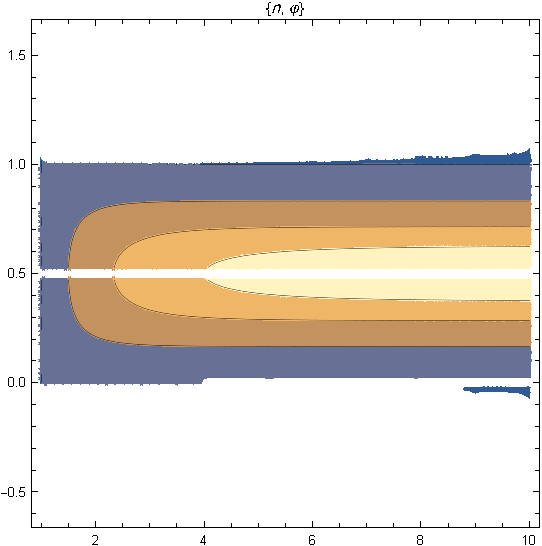
\includegraphics[width=0.5\linewidth]{Duaad2.pdf}
		\caption{Эмпирическая плотность символа $0$ в слове Фибоначчи для префиксов длины до $n=10$.}
		\label{jfig.2}
	\end{figure}
	\begin{figure}[H]
		\centering
		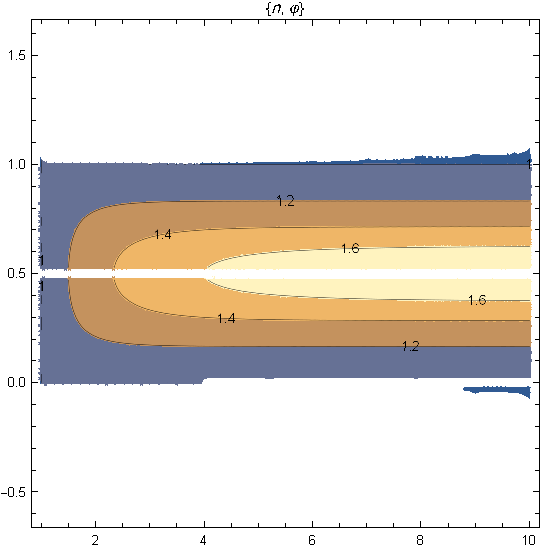
\includegraphics[width=0.5\linewidth]{Duaad3.pdf}
		\caption{Расширенное распределение плотности слова Фибоначчи, развивающее рисунок~\ref{jfig.2}.}
		\label{jfig.3}
	\end{figure}
	\begin{figure}[H]
		\centering
		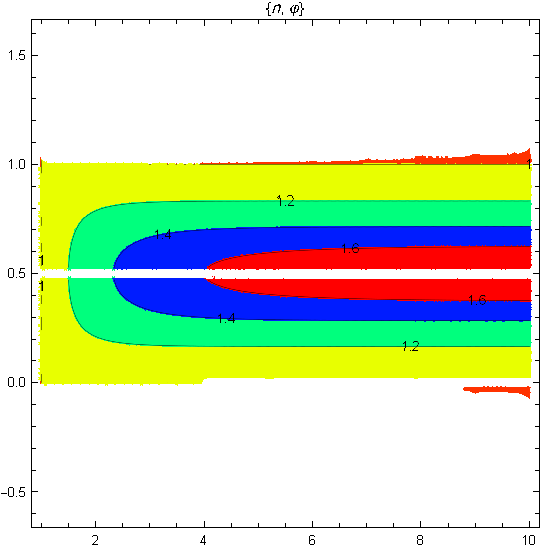
\includegraphics[width=0.5\linewidth]{Duaad4.pdf}
		\caption{Представление плотности слова Фибоначчи на основе цветовых оттенков для длины $n=10$.}
		\label{jfig.4}
	\end{figure}
\end{remark}
%-------------------------------------------------
\subsection{Плотности в факторах: обращение, сбалансированность, палиндромы}~\label{sec3.4.2}

Обращение слова не меняет числа вхождений любой буквы в него, поэтому плотности букв слова и его обращения совпадают. (Заметим, что \emph{обращение} слова не является палиндромом; палиндром --- это слово, равное своему обращению.)

\begin{proposition}\label{prop:balance}
	Пусть $\alpha=1/\varphi^{2}$. Каждый фактор $w$ слова $\mathbf f$ длины $m$ удовлетворяет условиям
	$|w|_1\in\{\lfloor m\alpha\rfloor,\lceil m\alpha\rceil\}$ и
	$|w|_0\in\{\lfloor m/\varphi\rfloor,\lceil m/\varphi\rceil\}$. Следовательно,
	\begin{equation}
		\Bigl|\frac{|w|_1}{m}-\frac1{\varphi^{2}}\Bigr|<\frac1m,\qquad
		\Bigl|\frac{|w|_0}{m}-\frac1{\varphi}\Bigr|<\frac1m ,
	\end{equation}
	как для палиндромных, так и для непалиндромных факторов.
\end{proposition}

\begin{proof}
	Пусть $w=c(i+1)\cdots c(i+m)$ и $x=(i+1)\alpha$. По предложению~\ref{prop:mech}
	$|w|_1=\lfloor x+m\alpha\rfloor-\lfloor x\rfloor\in\{\lfloor m\alpha\rfloor,\lfloor m\alpha\rfloor+1\}$,
	и $\lfloor m\alpha\rfloor+1=\lceil m\alpha\rceil$, поскольку $\alpha$ иррационально.
	Утверждение для $0$ следует из равенств $|w|_0=m-|w|_1$ и $1-\alpha=1/\varphi$.
\end{proof}

\noindent Оценка из предложения~\ref{prop:balance} была сформулирована без доказательства в~\cite{HamoudAbdullahTver} (предложение~8); доказательство через механическое представление, точный подсчёт из теоремы~\ref{mainre} и оптимальность его констант приведены здесь.

Например, каждый фактор длины $29$ слова $\mathbf f$ содержит $17$ или $18$ нулей. В частности, средние плотности $0$ и $1$, вычисленные
по факторам ограниченной длины, палиндромным или нет, отличаются от $1/\varphi$ и $1/\varphi^{2}$
не более чем на $1/m$, чем объясняется близость, наблюдаемая в численных экспериментах; никакого структурного
различия между палиндромными и непалиндромными факторами здесь не возникает.
%-----------------------------------------------
\subsection{Плотности коротких факторов}~\label{sec3.4.3}

\begin{example}
	Префиксы $s_n$ бесконечного слова Фибоначчи $\mathbf{f}$ таковы:
	\begin{equation}\label{fib}
		0,\ 01,\ 010,\ 01001,\ 01001010,\ 0100101001001,\dots
	\end{equation}
	Можно взять достаточно длинные префиксы слова $\mathbf{f}$ и подсчитать число вхождений каждого фактора
	длины $k\le 29$, чтобы сравнить эмпирические плотности с приведёнными выше предельными значениями.
\end{example}

\begin{example}
	Рассмотрим фактор $u=010$ в префиксе $p_{1000}$ длины $1000$ слова $\mathbf f$.
	Прямое вычисление даёт $381$ вхождение $u$, поэтому
	\begin{equation}
		\mathscr{D}_{1000}(010) = \frac{381}{1000} = 0.381 .
	\end{equation}
	Если вместо этого использовать число возможных начальных позиций, получим
	$\dfrac{381}{998} \approx 0.3818$.
	Поскольку $11$ не встречается в $\mathbf f$, каждая $1$, имеющая букву с каждой стороны, является серединой вхождения $010$, так что вхождения $010$ соответствуют вхождениям $1$ с одним краевым эффектом: $p_{1000}$ содержит $\lfloor 1001/\varphi^{2}\rfloor=382$ единицы, но последняя из них находится на позиции $1000$, и за ней не следует буква, поэтому вхождений $010$ только $381$. В пределе краевой эффект исчезает, и $\operatorname{freq}(010)=\operatorname{freq}(1)=1/\varphi^{2}\approx0.381966$.
\end{example}

\begin{example}\label{ex:freq-101}
	В префиксе $p_{1000}$ фактор $101$ встречается $145$ раз, так что $\mathscr D_{1000}(101)=0.145$.
	Это согласуется с точным значением $\operatorname{freq}(101)=1/\varphi^{4}\approx0.145898$.
\end{example}

\begin{proof}
	Факторы $11$ и $000$ не встречаются в $\mathbf f$. Следовательно, за каждой $1$ следует $0$ и ей предшествует $0$, каждому $00$ предшествует $1$, и, используя теорему~\ref{mainre},
	\begin{align}
		\operatorname{freq}(10)&=\operatorname{freq}(1)=\frac1{\varphi^{2}},\\
		\operatorname{freq}(00)&=\operatorname{freq}(0)-\operatorname{freq}(01)=\frac1\varphi-\frac1{\varphi^{2}},\\
		\operatorname{freq}(100)&=\operatorname{freq}(00).
	\end{align}
	За каждым вхождением $10$ следует $0$ или $1$, поэтому
	\begin{equation}
		\operatorname{freq}(101)=\operatorname{freq}(10)-\operatorname{freq}(100)
		=\frac{2}{\varphi^{2}}-\frac1\varphi=\frac{2-\varphi}{\varphi^{2}}=\frac1{\varphi^{4}} .
	\end{equation}
	Значение $145$ было получено порождением $p_{1000}$ с помощью морфизма $\Theta$ и подсчётом
	всех позиций $i$, для которых $\mathbf f[i]\mathbf f[i+1]\mathbf f[i+2]=101$.
\end{proof}

\begin{example}\label{thm6.2}
	В следующей таблице приведены плотности палиндромных факторов длины $2$, $3$ и $4$
	в префиксах $s_4$, $s_5$ и $s_6$ слова $\mathbf f$ (длин $8$, $13$ и $21$).
	\begin{table}[ht!]
		\centering
		\caption{Плотности палиндромных факторов длин $2$, $3$, $4$ в префиксах слова Фибоначчи.}\label{tab1}
		\begin{tabular}{|c|c|c|c|}
			\hline\hline
			\textbf{Длина} & \textbf{Палиндром} & \textbf{Префикс} & \textbf{Плотность} \\ \hline\hline
			2 & $00$   & $s_4$ & $1/8$  \\ \hline
			3 & $101$  & $s_5$ & $1/13$ \\ \hline
			3 & $010$  & $s_5$ & $4/13$ \\ \hline
			4 & $1001$ & $s_6$ & $4/21$ \\ \hline
		\end{tabular}
	\end{table}
\end{example}

\begin{proof}[Вычисление]
	\emph{Длина 2.} Двоичными палиндромами длины $2$ являются $00$ и $11$. В $\mathbf f$ фактор
	$11$ не встречается никогда, тогда как $00$ встречается. В префиксе $s_4=01001010$ палиндром $00$ появляется ровно один раз, так что
	$\mathscr{D}(00,s_4)=1/8=0.125$. Действительно, $1$ в $\mathbf f$ всегда изолирована между $0$.
	
	\emph{Длина 3.} Палиндромами длины $3$ являются $000,010,101,111$; факторы $000$ и $111$
	не встречаются. В $s_5=0100101001001$ (длины $13$) фактор $101$ встречается $1$ раз, а $010$ --- $4$ раза:
	\begin{equation}
		\mathscr{D}(101,s_5) = \frac{1}{13} \approx 0.077, \quad \mathscr{D}(010,s_5) = \frac{4}{13} \approx 0.308.
	\end{equation}
	
	\emph{Длина 4.} Двоичными палиндромами длины $4$ являются $0000, 0110, 1001, 1111$. Факторы
	$0000$, $1111$ и $0110$ не встречаются (последний --- потому что содержит $11$). В $s_6$ (длины $21$) палиндром
	$1001$ встречается $4$ раза: $\mathscr{D}(1001,s_6) = 4/21 \approx 0.190$.
	
	Эти значения являются плотностями в префиксах разных длин и несопоставимы друг с другом.
	Предельными частотами являются $\operatorname{freq}(010)=1/\varphi^{2}$ и $\operatorname{freq}(101)=1/\varphi^{4}$ (см. выше).
\end{proof}
%--------------------------------------------
\subsection{Количество палиндромных подслов каждой длины: эмпирические наблюдения в сопоставлении с теорией}~\label{sec3.4.4}

Начнём с напоминания хорошо известной характеризации штурмовых слов через палиндромную сложность.

\begin{proposition}
	Пусть $w$ --- бесконечное слово. Тогда $w$ является штурмовым тогда и только тогда, когда его палиндромная сложность удовлетворяет условию
	\begin{equation}
		P(n) =
		\begin{cases}
			1, & \text{если $n$ чётно},\\[2pt]
			2, & \text{если $n$ нечётно},
		\end{cases}
	\end{equation}
	для всех $n \ge 0$~\cite{DroubayX,Vuillon}.
\end{proposition}

Поскольку слово Фибоначчи $\mathbf{f}$ является штурмовым, его палиндромная сложность следует этой формуле.
Следующая таблица иллюстрирует это: в ней указаны числа различных палиндромных факторов каждой длины
$L\le 30$, встречающихся в префиксе $s_9$ слова $\mathbf f$ (длины $89$), который содержит все факторы слова
$\mathbf f$ длины не более $30$. Здесь $\operatorname{SL}$ --- длина, а
$\operatorname{NPS}$ --- число палиндромных подслов этой длины.
\begin{table}[H]
	\centering
	\begin{tabular}{|c|c||c|c|}
		\hline
		$\operatorname{SL}$ & $\operatorname{NPS}$   & $\operatorname{SL}$ & $\operatorname{NPS}$ \\
		\hline
		1 & 2 & 11 & 2 \\
		2 & 1 & 12 & 1 \\
		3 & 2 & 13 & 2 \\
		4 & 1 & 14 & 1 \\
		5 & 2 & 15 & 2 \\
		6 & 1 & 16 & 1 \\
		7 & 2 & 17 & 2 \\
		8 & 1 & 18 & 1 \\
		9 & 2 & 19 & 2 \\
		10 & 1 & 20 & 1 \\
		21 & 2 & 26 & 1 \\
		22 & 1 & 27 & 2 \\
		23 & 2 & 28 & 1 \\
		24 & 1 & 29 & 2 \\
		25 & 2 & 30 & 1 \\
		\hline
	\end{tabular}
	\caption{Число различных палиндромных подслов каждой длины, встречающихся в префиксе $s_9$ слова Фибоначчи.}
	\label{tab1duaamade}
\end{table}

Закономерность --- два палиндрома для нечётных длин и один для чётных --- согласуется с приведённым выше классическим
результатом; например, имеются два палиндромных фактора при $L=1,3,21,27,29$ и один при $L=2,8,12,16,30$.
%-----------------------------------------------
\subsection{Количества букв в конечных словах Фибоначчи}~\label{sec3.4.5}

Пусть $N_0(w)$ и $N_1(w)$ обозначают число нулей и единиц в слове $w$. Для $s_k=\Theta^k(0)$ имеем
$N_0(s_k)=F_{k+1}$, $N_1(s_k)=F_k$ и $|s_k|=F_{k+2}$, следовательно,
\begin{equation}
	\mathscr D(0,s_k)=\frac{F_{k+1}}{F_{k+2}}\to\frac1\varphi,\qquad
	\mathscr D(1,s_k)=\frac{F_{k}}{F_{k+2}}\to\frac1{\varphi^{2}}\qquad(k\to\infty),
\end{equation}
в соответствии с теоремой~\ref{mainre}. В таблице~\ref{tab1densityfibwo} приведены первые значения; плотности
быстро сходятся к $0.618$ и $0.382$.

\begin{table}[H]
	\centering
	\begin{tabular}{|c|c|c|c|c||c|c|c|c|c|}
		\hline
		$s_k$ & $N_0$ & $N_1$ & $\mathscr D_0$ & $\mathscr D_1$ & $s_k$ & $N_0$ & $N_1$ & $\mathscr D_0$ & $\mathscr D_1$ \\
		\hline
		$s_0$ & 1 & 0 & 1.000 & 0.000 & $s_1$ & 1 & 1 & 0.500 & 0.500 \\
		$s_2$ & 2 & 1 & 0.667 & 0.333 & $s_3$ & 3 & 2 & 0.600 & 0.400 \\
		$s_4$ & 5 & 3 & 0.625 & 0.375 & $s_5$ & 8 & 5 & 0.615 & 0.385 \\
		$s_6$ & 13 & 8 & 0.619 & 0.381 & $s_7$ & 21 & 13 & 0.618 & 0.382 \\
		$s_8$ & 34 & 21 & 0.618 & 0.382 & $s_9$ & 55 & 34 & 0.618 & 0.382 \\
		$s_{13}$ & 377 & 233 & 0.618 & 0.382 & $s_{14}$ & 610 & 377 & 0.618 & 0.382 \\
		$s_{18}$ & 4181 & 2584 & 0.618 & 0.382 & $s_{19}$ & 6765 & 4181 & 0.618 & 0.382 \\
		\hline
	\end{tabular}
	\caption{Количества и плотности нулей и единиц в словах Фибоначчи $s_k$.}
	\label{tab1densityfibwo}
\end{table}

Эти значения были также получены с помощью алгоритма~\ref{algorithm1}, который порождает $s_k$ и вычисляет
плотность выбранной буквы.

\begin{algorithm}[H]
	\caption{Алгоритм вычисления плотности букв в словах Фибоначчи}\label{algorithm1}
	\begin{algorithmic}[1]
		\Procedure{GenerateFibonacciWord}{$k$}
		\If{$k = 0$}
		\State \Return ``0''
		\ElsIf{$k = 1$}
		\State \Return ``01''
		\Else
		\State \Return \Call{GenerateFibonacciWord}{$k-1$} \textbf{конкатенированное с} \Call{GenerateFibonacciWord}{$k-2$}
		\EndIf
		\EndProcedure
		
		\Function{CalculateDensity}{$fib\_word, char$}
		\State $count \gets$ число вхождений $char$ в $fib\_word$
		\State \Return $count / \text{length}(fib\_word)$
		\EndFunction
		
		\Procedure{Main}{$max\_k, char$}
		\For{$i = 0$ \textbf{до} $max\_k$}
		\State $fib\_w \gets$ \Call{GenerateFibonacciWord}{$i$}
		\State $dens \gets$ \Call{CalculateDensity}{$fib\_w, char$}
		\State \textbf{вывести} ``D(s\_$i$) = $dens$''
		\EndFor
		\EndProcedure
	\end{algorithmic}
\end{algorithm}
%-------------------------------------------------
\section{Механическое описание, производящая функция и обрамлённые слова}~\label{sec3.5}
%-----------------------------------------------
\noindent\textit{Части этой главы основаны на опубликованной работе автора~\cite{HamoudAbdullah}.}

%-----------------------
\subsection{Теоретические основы и динамика плотностей}~\label{sec3.5.1}
\label{sec02}
В этом разделе мы изучаем плотности букв слова Фибоначчи $\mathbf f$ с механической (битти) точки зрения, описываем его локальную структуру, напоминаем результаты о его производящей функции	и изучаем, как изменяются плотности букв при добавлении граничных букв к конечным
словам Фибоначчи (обрамлённые слова). Всюду далее $F_n$ --- числа Фибоначчи ($F_0=0$, $F_1=1$),
$\varphi=\frac{1+\sqrt5}{2}$, $\psi=\frac{1-\sqrt5}{2}=-\varphi^{-1}$, а $\mathbf f=\lim_n s_n$,
$s_n=\Theta^n(0)$ --- как в разделе~3.2; в этом разделе позиции слова $\mathbf f$ нумеруются начиная с 	$1$, $\mathbf f=\mathbf f[1]\mathbf f[2]\mathbf f[3]\cdots=0100101001001\cdots$. 

%=====================
\subsection{Механическое описание и локальная структура}\label{sec:main}~\label{sec3.5.2}
%=====================

Пусть $B_1=\{\lfloor m\varphi\rfloor : m\ge1\}=\{1,3,4,6,8,9,\dots\}$ и
$B_2=\{\lfloor m\varphi^2\rfloor : m\ge1\}=\{2,5,7,10,13,\dots\}$. По теореме Битти~\cite{Beatty1926}
множества $B_1$ и $B_2$ образуют разбиение $\mathbb N_{\ge1}$ (заметим, что $1/\varphi+1/\varphi^2=1$).

\begin{lemma}[Механическое описание слова $\mathbf f$]\label{lem:mechanical}
	Для каждого $n\ge1$
	\begin{equation}
		\mathbf f[n]=1\iff n\in B_2,\qquad \mathbf f[n]=0\iff n\in B_1 .
	\end{equation}
	Другими словами, единицы слова $\mathbf f$ находятся на позициях $\lfloor m\varphi^2\rfloor$, а нули --- на позициях $\lfloor m\varphi\rfloor$.
\end{lemma}

\begin{proof}
	Пусть $\alpha=\varphi^{-2}$. По предложению~\ref{prop:mech} (раздел~3.4) $\mathbf f[n]=\lfloor (n+1)\alpha\rfloor-\lfloor n\alpha\rfloor\in\{0,1\}$.
	Она равна $1$ тогда и только тогда, когда существует целое $m$, для которого $n\alpha<m\le(n+1)\alpha$, т.е.\ $n<m\varphi^{2}\le n+1$.
	Поскольку $m\varphi^2$ иррационально, это означает, что $n<m\varphi^2<n+1$, т.е.\ $n=\lfloor m\varphi^2\rfloor$.
	Утверждение для $0$ следует из того, что $B_1\cup B_2=\mathbb N_{\ge1}$ является дизъюнктным объединением.
\end{proof}

\begin{remark}
	Естественная плотность множества $\{\lfloor m\theta\rfloor\}$ равна $1/\theta$; следовательно, нули имеют плотность $1/\varphi$, а единицы имеют плотность
	$1/\varphi^{2}$, в соответствии с теоремой~\ref{mainre}, которая также даёт оценку уклонения
	$\bigl||p_n|_1-n/\varphi^{2}\bigr|<1$ для каждого префикса $p_n$ длины $n$.
\end{remark}

\begin{corollary}\label{thm:density}\label{thm:prefix-density}\label{thm:summary-density}
	$\delta_0(\mathbf f)=1/\varphi$, $\delta_1(\mathbf f)=1/\varphi^{2}$, и $|p_n|_1=n/\varphi^{2}+O(1)$,
	$|p_n|_0=n/\varphi+O(1)$.
\end{corollary}

\begin{lemma}[Локальная структура]\label{lem:local}
	В бесконечном слове Фибоначчи $\mathbf f$:
	\begin{itemize}
		\item[(i)] фактор $11$ не встречается;
		\item[(ii)] фактор $000$ не встречается;
		\item[(iii)] каждый фактор длины $3$ содержит один или два символа $1$. Факторами длины $3$ являются в точности
		$001,\ 010,\ 100$ (одна $1$) и $101$ (две $1$).
	\end{itemize}
\end{lemma}

\begin{proof}
	По лемме~\ref{lem:mechanical} единицы находятся на позициях $b_m=\lfloor m\varphi^2\rfloor$, и
	$b_{m+1}-b_m\in\{\lfloor\varphi^2\rfloor,\lceil\varphi^2\rceil\}=\{2,3\}$. Расстояние $\ge2$ даёт (i); расстояние $\le3$ означает не более двух
	подряд идущих нулей, что даёт (ii). Слово длины $3$ без $11$ и $000$ является одним из
	$001,010,100,101$; все четыре встречаются в префиксе $01001010$.
\end{proof}

\begin{remark}
	Среднее число единиц в факторе длины $3$ равно $3/\varphi^{2}\approx1.146$, что согласуется с (iii) и
	с предложением~\ref{prop:balance}: $|w|_1\in\{\lfloor 3\alpha\rfloor,\lceil3\alpha\rceil\}=\{1,2\}$.
\end{remark}

Механическое описание из леммы~\ref{lem:mechanical} можно визуализировать, построив графики последовательностей Битти
\begin{equation}
	g_1(n) = \lfloor n\varphi \rfloor,
	\qquad
	g_2(n) = \lfloor n\varphi^2 \rfloor,
\end{equation}
которые задают позиции символов $0$ и $1$ в $\mathbf f$ соответственно.

\begin{figure}[H]
	\centering
	\begin{tikzpicture}[scale=1.2]
		\begin{axis}[
			legend pos=north west,
			grid=major,
			enlargelimits=0.1,
			]
			\addplot[blue, mark=*] coordinates {
				(1,1) (2,3) (3,4) (4,6) (5,8) (6,9) (7,11) (8,12) (9,14) (10,16) (11,17)
				(12,19) (13,21) (14,22) (15,24) (16,25) (17,27) (18,29) (19,30) (20,32)
				(21,33) (22,35) (23,37) (24,38) (25,40) (26,42) (27,43) (28,45) (29,46)
				(30,48)
			};
			\addlegendentry{$g_1(n)=\lfloor n\varphi \rfloor$}
			
			\addplot[red, mark=triangle*] coordinates {
				(1,2) (2,5) (3,7) (4,10) (5,13) (6,15) (7,18) (8,20) (9,23) (10,26) (11,28)
				(12,31) (13,34) (14,36) (15,39) (16,41) (17,44) (18,47) (19,49) (20,52)
				(21,54) (22,57) (23,60) (24,62) (25,65) (26,68) (27,70) (28,73) (29,75)
				(30,78)
			};
			\addlegendentry{$g_2(n)=\lfloor n\varphi^2 \rfloor$}
		\end{axis}
	\end{tikzpicture}
	\caption{Последовательности Битти, задающие позиции $0$ и $1$ в слове Фибоначчи (лемма~\ref{lem:mechanical}).}
	\label{fig002DuaaAvf}
\end{figure}

%-------------------------------------------------
\subsection{Производящая функция слова Фибоначчи}~\label{sec3.5.3}
%-------------------------------------------------
\begin{proposition}[известные результаты]\label{sec2:proposition1}
	Пусть $\mathcal F(z)=\sum_{n\ge1}\mathbf f[n]\,z^n$ при $|z|<1$. Тогда:
	\begin{enumerate}
		\item $\mathcal F(z)=\sum_{m\ge1}z^{\lfloor m\varphi^2\rfloor}$;
		\item $\mathcal F$ не является рациональной функцией;
		\item для каждого целого $b\ge2$ число $\mathcal F(1/b)=\sum_{n\ge1}\mathbf f[n]\,b^{-n}$ трансцендентно.
	\end{enumerate}
\end{proposition}

\begin{proof}
	(1) следует из леммы~\ref{lem:mechanical}. (2) Коэффициенты рационального степенного ряда финально периодичны,
	тогда как $\mathbf f$ непериодично. (3) $\mathcal F(1/b)$ --- это число, $b$-ичным разложением которого является штурмово слово $\mathbf f$;
	его трансцендентность есть теорема Ференци и Моди~\cite{Ferenczi}, см. также Адамчевский, Бюжо и Ференци–Моди~\cite{AdamczewskiB2007,Fogg}.
\end{proof}

\begin{remark}
	Утверждение~(3) сформулировано только для $z=1/b$, что и покрывается цитируемыми теоремами. Утверждение для всех алгебраических $z$ при $0<|z|<1$
	потребовало бы отдельной ссылки и здесь не заявляется.
\end{remark}
%-------------------------------------------------
\subsection{Обрамлённые слова Фибоначчи и граничные возмущения}~\label{sec3.5.4}
%------------------------------------------------
Слова $u_n$ и $q_m$ и первая форма теоремы~\ref{thm1Asymptotic} (пределы $1/\varphi$, $1/\varphi^2$) были введены в совместной работе~\cite{HamoudAbdullah}; точная формула для остаточного члена, утверждение о знаке и исправленная числовая таблица являются новыми.

В этом подразделе мы записываем слова Фибоначчи над алфавитом $\{a,b\}$: пусть $u_n$ --- образ $s_n$ при отображении $0\mapsto a$, $1\mapsto b$, т.е.\
\begin{equation}\label{eq1defnewwordn1}
	u_0=a,\ u_1=ab,\ u_n=u_{n-1}u_{n-2}.
\end{equation}
\begin{definition}[Фибоначчиподобные слова $\mathbb U=(u_n)_{n\ge0}$]\label{defnewwordn1}
	Слова $u_n$ являются префиксами $\Theta^n(a)$ неподвижной точки морфизма $\Theta\colon a\mapsto ab,\ b\mapsto a$.
\end{definition}

\begin{proposition}\label{pro1defnewwordn1}
	Для каждого $n\ge0$: $|u_n|=F_{n+2}$, $|u_n|_a=F_{n+1}$, $|u_n|_b=F_n$.
\end{proposition}
\begin{proof}
	Эти три величины удовлетворяют соотношению $X_n=X_{n-1}+X_{n-2}$ (поскольку $u_n=u_{n-1}u_{n-2}$), при этом $|u_0|=1=F_2$, $|u_1|=2=F_3$,
	$(|u_0|_a,|u_0|_b)=(1,0)=(F_1,F_0)$, $(|u_1|_a,|u_1|_b)=(1,1)=(F_2,F_1)$.
\end{proof}

\begin{definition}[Обрамлённые слова $\mathbb Q=(q_m)_{m\ge1}$]\label{defnewwordn2}
	$q_m=a\,u_m\,b$ при $m\ge1$.
\end{definition}

\begin{proposition}\label{pro1defnewwordn2}
	$|q_m|=F_{m+2}+2$, $\ |q_m|_a=F_{m+1}+1$, $\ |q_m|_b=F_m+1$.
\end{proposition}
\begin{proof}
	Непосредственно следует из равенства $|q_m|=1+|u_m|+1$ и предложения~\ref{pro1defnewwordn1}.
\end{proof}

Например,
\begin{align}
	q_1 &= a(ab)b = aabb,\\
	q_2 &= a(aba)b = aabab,\\
	q_3 &= a(abaab)b = aabaabb .
\end{align}

\begin{theorem}[Плотности в обрамлённых словах]\label{thm1Asymptotic}
	Пусть $\operatorname{dens}_c(w)=|w|_c/|w|$. Для каждого $m\ge1$
	\begin{equation}
		\operatorname{dens}_a(q_m)=\frac{F_{m+1}+1}{F_{m+2}+2}=\frac1\varphi-\frac{\varphi^{-2}+\psi^{m+1}}{\varphi\,(F_{m+2}+2)},
		\qquad
		\operatorname{dens}_b(q_m)=1-\operatorname{dens}_a(q_m).
	\end{equation}
	Следовательно, $\operatorname{dens}_a(q_m)\to1/\varphi$, $\operatorname{dens}_b(q_m)\to1/\varphi^{2}$ с погрешностью
	$O(1/F_{m+2})=O(\varphi^{-m})$, и $\operatorname{dens}_a(q_m)<1/\varphi$ при всех $m\ge1$.
\end{theorem}

\begin{proof}
	Первое равенство есть предложение~\ref{pro1defnewwordn2}. Из формулы Бине $F_{n+1}-\varphi F_n=\psi^n$, поэтому
	\begin{equation}
		\varphi(F_{m+1}+1)-(F_{m+2}+2)=-\psi^{m+1}+(\varphi-2)=-(\psi^{m+1}+\varphi^{-2}),
	\end{equation}
	так как $2-\varphi=\varphi^{-2}$. Деление на $\varphi(F_{m+2}+2)$ даёт формулу. При $m\ge1$ имеем $|\psi|^{m+1}\le\varphi^{-2}$,
	так что $\psi^{m+1}+\varphi^{-2}>0$ (при $m=1$: $\psi^2+\varphi^{-2}=2\varphi^{-2}$), откуда следует утверждение о знаке. Наконец, $F_{m+2}\sim\varphi^{m+2}/\sqrt5$.
\end{proof}

Для необрамлённых слов имеем $\operatorname{dens}_a(u_m)=F_{m+1}/F_{m+2}$ и
$\operatorname{dens}_a(u_m)-1/\varphi=-\psi^{m+1}/(\varphi F_{m+2})$, что меняет знак (чередуется) и есть $O(\varphi^{-2m})$.
Таким образом, одна граничная буква с каждой стороны замедляет сходимость с $O(\varphi^{-2m})$ до $O(\varphi^{-m})$
и делает её односторонней. В таблице~\ref{tab002densitiesASm} приведены значения.

\begin{table}[H]
	\centering
	\small
	\begin{tabular}{ccccc}
		\hline
		$m$ & $\text{dens}_a(q_m)$ & $\text{dens}_b(q_m)$ & $\text{dens}_a(u_m)$ & $\text{dens}_b(u_m)$ \\ \hline
		3  & 0.571429 & 0.428571 & 0.600000 & 0.400000 \\
		5  & 0.600000 & 0.400000 & 0.615385 & 0.384615 \\
		7  & 0.611111 & 0.388889 & 0.617647 & 0.382353 \\
		9  & 0.615385 & 0.384615 & 0.617978 & 0.382022 \\
		11 & 0.617021 & 0.382979 & 0.618026 & 0.381974 \\
		13 & 0.617647 & 0.382353 & 0.618033 & 0.381967 \\ \hline
		$\infty$ & 0.618034 & 0.381966 & 0.618034 & 0.381966 \\ \hline
	\end{tabular}
	\caption{Плотности букв в обрамлённых словах $q_m$ и в словах $u_m$.}
	\label{tab002densitiesASm}
\end{table}
%-----------------------------------------------
\subsection{Телескопический ряд с дважды экспоненциальной сходимостью}\label{sec:millin}

\begin{lemma}\label{lem:telesc}
	При $n\ge1$: $\dfrac{F_{n-1}}{F_n}-\dfrac{F_{2n-1}}{F_{2n}}=\dfrac{(-1)^n}{F_{2n}}$.
\end{lemma}
\begin{proof}
	$F_{2n}=F_n(F_{n+1}+F_{n-1})$ и $F_{2n-1}=F_n^2+F_{n-1}^2$. Приведя к знаменателю $F_{2n}$,
	получаем числитель $F_{n-1}(F_{n+1}+F_{n-1})-F_n^2-F_{n-1}^2=F_{n-1}F_{n+1}-F_n^2=(-1)^n$ (Кассини).
\end{proof}

\begin{theorem}\label{thm:millin}
	Для каждого $m\ge1$
	\begin{equation}
		\sum_{k=1}^{\infty}\frac1{F_{m2^k}}=\frac{F_{m-1}}{F_m}-\frac1\varphi+\frac{1-(-1)^m}{F_{2m}} .
	\end{equation}
	Точнее, при $M=m2^{K+1}$
	$\displaystyle\sum_{k=1}^{K+1}\frac1{F_{m2^k}}=\frac{F_{m-1}}{F_m}-\frac{F_{M-1}}{F_M}+\frac{1-(-1)^m}{F_{2m}}$,
	и $F_{M-1}/F_M=\varphi^{-1}-\psi^{M-1}/(\varphi F_M)$, так что остаток после $K+1$ слагаемых есть $O(\varphi^{-2^{K}m})$ (дважды экспоненциально мал).
\end{theorem}

\begin{proof}
	Применим лемму~\ref{lem:telesc} при $n=m2^j$, $j=0,\dots,K$, и сложим. Левые части телескопируются:
	\begin{equation}
		\sum_{j=0}^{K}\frac{(-1)^{m2^j}}{F_{m2^{j+1}}}=\frac{F_{m-1}}{F_m}-\frac{F_{M-1}}{F_M},\qquad M=m2^{K+1}.
	\end{equation}
	При $j=0$ знак равен $(-1)^m$; при $j\ge1$ показатель $m2^j$ чётен, поэтому знак равен $+$. Следовательно,
	\begin{equation}
		\sum_{j=0}^{K}\frac1{F_{m2^{j+1}}}=\frac{F_{m-1}}{F_m}-\frac{F_{M-1}}{F_M}+\Bigl(1-(-1)^m\Bigr)\frac1{F_{2m}},
	\end{equation}
	что и есть конечная формула (сумма слева есть $\sum_{k=1}^{K+1}1/F_{m2^k}$). Выражение для $F_{M-1}/F_M$ есть лемма~\ref{lem:fibA}.
\end{proof}

\begin{remark}
	При $m=1$ это даёт $\sum_{k\ge0}F_{2^k}^{-1}=\frac{7-\sqrt5}2$ (ряд Миллина~\cite{Millin}). Это тождество является стандартным обобщением классического
	телескопического рассуждения; мы не претендуем на новизну, кроме явной скорости сходимости.
\end{remark}
%------------------------------
\subsection{Два тождества для чисел Фибоначчи}\label{sec:identDF}

Здесь $F_0=0$, $F_1=1$ и $g_k=F_{k+1}/F_k$ ($k\ge1$), так что $g_k\to\varphi$. Эти тождества были сформулированы в~\cite{AbdullahHam}
(при индексации $F_0=F_1=1$); приведённые там доказательства неполны, и мы даём полные доказательства.

\begin{lemma}[д'Окань]\label{lem:docagne}
	При $k\ge1$, $m\ge0$: $F_{k+m}F_{k+1}-F_{k+m+1}F_k=(-1)^kF_m$. Следовательно, при $m\ge1$
	\begin{equation}
		\frac{(-1)^kF_m}{F_kF_{k+m}}=g_k-g_{k+m}.
	\end{equation}
\end{lemma}
\begin{proof}
	По формуле Бине левая часть равна
	$\frac15(\varphi\psi)^k(\varphi-\psi)(\varphi^m-\psi^m)=(-1)^kF_m$, так как $\varphi\psi=-1$, $\varphi-\psi=\sqrt5$ и $\varphi^m-\psi^m=\sqrt5F_m$.
	Разделим на $F_kF_{k+m}$.
\end{proof}

\begin{proposition}[симметрия]\label{prop:symm}
	Для всех целых $a,b\ge1$
	\begin{equation}
		\sum_{k=1}^{b}\frac{(-1)^kF_a}{F_kF_{k+a}}=\sum_{k=1}^{a}\frac{(-1)^kF_b}{F_kF_{k+b}} .
	\end{equation}
\end{proposition}
\begin{proof}
	Пусть $S(n)=\sum_{k=1}^n g_k$. По лемме~\ref{lem:docagne} левая часть равна $\sum_{k=1}^b(g_k-g_{k+a})=S(b)-(S(a+b)-S(a))=S(a)+S(b)-S(a+b)$, что симметрично относительно $a,b$.
\end{proof}

\begin{proposition}\label{prop:sum2r}
	Для каждого целого $r\ge1$
	\begin{equation}
		\sum_{k\ge1}\frac1{F_kF_{k+2r}}=\frac1{F_{2r}}\sum_{n=1}^{r}\frac1{F_{2n-1}F_{2n}} .
	\end{equation}
\end{proposition}
\begin{proof}
	По лемме~\ref{lem:docagne} при $m=2r$ и $(-1)^{k+2r}=(-1)^k$
	\begin{equation}
		F_{2r}\sum_{k=1}^{N}\frac1{F_kF_{k+2r}}=\sum_{k=1}^N(-1)^k(g_k-g_{k+2r})
		=\sum_{k=1}^{2r}(-1)^kg_k-\sum_{j=N+1}^{N+2r}(-1)^jg_j .
	\end{equation}
	Последняя сумма содержит $2r$ подряд идущих слагаемых с чередующимися знаками, каждое из которых стремится к $\varphi$, поэтому она стремится к $0$. Кроме того,
	$\sum_{k=1}^{2r}(-1)^kg_k=\sum_{n=1}^r(g_{2n}-g_{2n-1})=\sum_{n=1}^r\frac1{F_{2n-1}F_{2n}}$ по лемме~\ref{lem:docagne} ($m=1$).
\end{proof}
%--------------------------------------------------
\section{Об асимптотической палиндромной плотности бесконечных слов Фибоначчи}~\label{sec3.6}

Пусть $A$ --- конечный алфавит. Конечное слово $w$ длины $n$ над $A$ --- это последовательность
$w=w_0w_1\cdots w_{n-1}$~\cite{Rigo}; $|w|$ обозначает его длину, а $A^*$ --- множество всех конечных слов.
\emph{Обращением} слова $w$ называется слово $w^R=w_{n-1}\cdots w_1w_0$, а \emph{палиндромом} --- слово $w$, для которого $w=w^R$.
Для бесконечного слова $\mathbf w$ нас интересуют его палиндромные префиксы. Фишлер~\cite{Fischler} ввёл
асимптотическую палиндромную плотность: если $(n_i)_{i\ge0}$ --- возрастающая последовательность длин всех палиндромных
префиксов слова $\mathbf w$, то
\begin{equation}\label{eqqintron1}
	\mathrm{dens}_p(\mathbf w):=\Bigl(\limsup_{i\to\infty}\frac{n_{i+1}}{n_i}\Bigr)^{-1},
\end{equation}
с соглашением $\mathrm{dens}_p(\mathbf w):=0$, если у $\mathbf w$ лишь конечное число палиндромных префиксов.
Очевидно, $0\le\mathrm{dens}_p(\mathbf w)\le1$. В этом разделе $\varphi=\frac{1+\sqrt5}2$ всегда обозначает
золотое сечение, а морфизм Фибоначчи обозначается $\Theta$ (раздел~3.2). 	
%-----------------------------------------
\subsection{Штурмовы слова и слово Фибоначчи}~\label{sec3.6.1}	

\begin{definition}[Штурмовы слова~\cite{Lothaire2002}]\label{deffSturmiann1}
	Пусть $\alpha\in(0,1)$ иррационально и $\beta\in[0,1)$. Слова
	$u_n=\lfloor\alpha(n+1)+\beta\rfloor-\lfloor\alpha n+\beta\rfloor$ ($n\ge0$) и
	$u'_n=\lceil\alpha(n+1)+\beta\rceil-\lceil\alpha n+\beta\rceil$ ($n\ge0$) называются \emph{штурмовыми словами с угловым коэффициентом $\alpha$}.
	\emph{Характеристическое слово} с угловым коэффициентом $\alpha$ получается в первой форме при $\beta=\alpha$; эквивалентно,
	$c_\alpha[n]=\lfloor(n+1)\alpha\rfloor-\lfloor n\alpha\rfloor$ при $n\ge1$.
\end{definition}

\begin{proposition}[\cite{Lothaire2002,Allouche}]\label{proirrationaln1}
	Пусть $\alpha=[0;1+d_1,d_2,d_3,\dots]$ иррационально. Положим $s_{-1}=1$, $s_0=0$ и $s_j=s_{j-1}^{d_j}s_{j-2}$ при $j\ge1$.
	Тогда $(s_j)$ сходится к характеристическому слову с угловым коэффициентом $\alpha$.
\end{proposition}

\begin{definition}[Слово Фибоначчи]\label{defffFibonaccin}
	Слово Фибоначчи --- это характеристическое слово с угловым коэффициентом $\alpha=1/\varphi^{2}=[0;2,1,1,1,\dots]$.
	По предложению~\ref{proirrationaln1} (все $d_j=1$) оно является пределом слов $s_n$, где
	$s_{-1}=1$, $s_0=0$, $s_n=s_{n-1}s_{n-2}$, как в разделе~3.2; оно начинается с
	\begin{equation}
		0\ 1\ 0\ 0\ 1\ 0\ 1\ 0\ 0\ 1\ 0\ 0\ 1\ 0\ \dots
	\end{equation}
\end{definition}

\begin{theorem}[\cite{Fischler}]\label{ThmplinDENSN1}
	Пусть $\mathbf w$ --- бесконечное непериодическое слово. Тогда
	\begin{equation}\label{eq1ThmplinDENSN1}
		\mathrm{dens}_p(\mathbf w)\le\frac1\varphi .
	\end{equation}
\end{theorem}
%-----------------------------------------
\subsection{Палиндромная плотность слова Фибоначчи}~\label{sec3.6.2}

Пусть $t_n$ --- слово $s_n$ с отброшенными двумя последними буквами ($n\ge1$); таким образом, $t_1=\varepsilon$, $t_2=0$, $t_3=010$,
$t_4=010010$, и $|t_n|=F_{n+2}-2$.

\begin{lemma}[Палиндромные префиксы слова Фибоначчи]\label{lem:palFib}
	Для каждого $n\ge1$ слово $t_n$ является палиндромом. Следовательно, у $\mathbf f$ есть палиндромный префикс длины
	$F_{n+2}-2$ для каждого $n\ge2$.
\end{lemma}

\begin{proof}
	Пусть $e_n$ обозначает две последние буквы слова $s_n$ ($n\ge1$). Поскольку $s_n=s_{n-1}s_{n-2}$, имеем $e_n=e_{n-2}$ при $n\ge3$,
	а $e_1=01$, $e_2=10$; следовательно, $e_{n}$ и $e_{n-1}$ являются обращениями друг друга.
	
	\emph{Утверждение.} При $n\ge1$ слова $s_ns_{n-1}$ и $s_{n-1}s_n$ совпадают всюду, кроме двух последних букв.
	При $n=1$: $s_1s_0=010$, $s_0s_1=001$. Если оно выполнено для $n$, то
	$s_{n+1}s_n=s_n\,(s_{n-1}s_n)$ и $s_ns_{n+1}=s_n\,(s_ns_{n-1})$ совпадают всюду, кроме двух последних букв.
	
	Теперь покажем индукцией, что $t_n$ является палиндромом. Это верно при $n=1,2$. Пусть $n\ge3$. Тогда
	$t_n=t_{n-1}\,e_{n-1}\,t_{n-2}$, и по утверждению $t_n$ также равно $s_{n-2}t_{n-1}=t_{n-2}\,e_{n-2}\,t_{n-1}$.
	По предположению индукции $t_{n-1},t_{n-2}$ являются палиндромами, и $e_{n-1}^R=e_{n-2}$, поэтому
	\begin{equation}
		t_n^R=t_{n-2}^R\,e_{n-1}^R\,t_{n-1}^R=t_{n-2}\,e_{n-2}\,t_{n-1}=t_n .
	\end{equation}
	Наконец, $t_n$ является префиксом слова $s_n$, а значит, и слова $\mathbf f$.
\end{proof}

\begin{remark}
	На самом деле числа $F_{n+2}-2$ --- это \emph{все} длины палиндромных префиксов слова $\mathbf f$ (де~Лука~\cite{DeLuca1997}); это используется в теореме~\ref{thm:Ypal}.
\end{remark}

\begin{theorem}[Палиндромная плотность слова Фибоначчи]\label{thm:palFib}
	$\mathrm{dens}_p(\mathbf f)=1/\varphi$.
\end{theorem}

\begin{proof}
	Пусть $a_k=F_{k+2}-2$ ($k\ge2$); по лемме~\ref{lem:palFib} каждое $a_k$ является длиной палиндромного префикса.
	Пусть $(n_i)$ --- возрастающая последовательность длин \emph{всех} непустых палиндромных префиксов слова $\mathbf f$; каждое $a_k$ встречается в ней.
	Для данного $i$ выберем $k$ так, что $a_k\le n_i<a_{k+1}$. Поскольку $a_{k+1}$ встречается в $(n_i)$ и $a_{k+1}>n_i$, получаем $n_{i+1}\le a_{k+1}$, следовательно,
	$n_{i+1}/n_i\le a_{k+1}/a_k\to\varphi$ (лемма~\ref{lem:fibA}); поэтому $\limsup n_{i+1}/n_i\le\varphi$.
	Поскольку $\mathbf f$ непериодическое, теорема~\ref{ThmplinDENSN1} даёт $\limsup n_{i+1}/n_i\ge\varphi$.
\end{proof}

Таким образом, слово Фибоначчи достигает оценки Фишлера; это значение принадлежит Фишлеру~\cite{Fischler}.

\begin{remark}[Плотность палиндромных префиксов не монотонна относительно сдвига]
	Плотность $\mathrm{dens}_p$ не монотонна относительно удаления префикса. Пусть $\mathbf w=2\mathbf f$, где $2$ --- буква,
	не встречающаяся в $\mathbf f$. Единственным палиндромным префиксом слова $\mathbf w$ является $2$, так что $\mathrm{dens}_p(\mathbf w)=0$,
	тогда как $\mathrm{dens}_p(\mathbf f)=1/\varphi$. 
\end{remark}
%--------------------------------------------
\subsection{Тернарное фибоначчиподобное слово}~\label{sec3.6.3}

Пусть $(y_n)_{n\ge0}$ --- слова над $\{0,1,2\}$, определённые равенствами
\begin{equation}
	y_0=01,\qquad y_1=02,\qquad y_n=y_{n-1}y_{n-2}\quad(n\ge2).
\end{equation}
Таким образом, $y_2=0201$, $y_3=020102$, $y_4=0201020201$. Каждая вторая буква слова $y_n$ есть $0$, и $y_n=h(z_n)$, где
$h(c)=0c$, а $(z_n)$ --- последовательность слов фибоначчиевского типа над $\{1,2\}$ с $z_0=1$, $z_1=2$, $z_n=z_{n-1}z_{n-2}$;
так что $y_n$ является простым кодированием слов фибоначчиевского типа. Положим $\lambda_n=|y_n|_0$, $\alpha_n=|y_n|_1$, $\beta_n=|y_n|_2$ и
$\mathcal L_n=|y_n|$.

\begin{proposition}\label{lemmanovelwordn1}
	Для $n\ge0$ (при $F_{-1}=1$): $\lambda_n=F_{n+1}$, $\alpha_n=F_{n-1}$, $\beta_n=F_n$, $\mathcal L_n=2F_{n+1}$.
	Следовательно, $\mathcal L_n/\mathcal L_{n-1}\to\varphi$.
\end{proposition}
\begin{proof}
	Все четыре последовательности удовлетворяют соотношению $X_n=X_{n-1}+X_{n-2}$, так как $y_n=y_{n-1}y_{n-2}$, и начальные значения
	$(\lambda_0,\alpha_0,\beta_0)=(1,1,0)=(F_1,F_{-1},F_0)$, $(\lambda_1,\alpha_1,\beta_1)=(1,0,1)=(F_2,F_0,F_1)$ согласуются.
	Последнее утверждение следует из $F_{n+1}/F_n\to\varphi$.
\end{proof}

\begin{corollary}\label{eq1densityn1}
	Пусть $\rho_n(s)=|y_n|_s/\mathcal L_n$. Тогда $\rho_n(0)=\tfrac12$ при всех $n$, и
	\begin{equation}
		\rho_n(1)=\frac{F_{n-1}}{2F_{n+1}}\longrightarrow\frac1{2\varphi^{2}}\approx0.19098,\qquad
		\rho_n(2)=\frac{F_n}{2F_{n+1}}\longrightarrow\frac1{2\varphi}\approx0.30902 .
	\end{equation}
\end{corollary}

\begin{figure}[H]
	\centering
	\begin{tikzpicture}
		\begin{axis}[
			ybar,
			bar width=8pt,
			width=13cm,
			height=8cm,
			xmin=-0.75, xmax=12.75,
			xtick={0,...,12},
			xlabel={$n$},
			ylabel={Относительная частота},
			ymin=0, ymax=0.6,
			legend style={at={(0.5,1.05)},anchor=south,legend columns=3}
			]
			\addplot+[fill=blue!70!black] coordinates {
				(0,0.5) (1,0.5) (2,0.5) (3,0.5) (4,0.5)
				(5,0.5) (6,0.5) (7,0.5) (8,0.5) (9,0.5)
				(10,0.5) (11,0.5) (12,0.5)
			};
			\addplot+[fill=red!70!black] coordinates {
				(0,0.5) (1,0.0) (2,0.25) (3,0.166666667) (4,0.2)
				(5,0.1875) (6,0.192307692) (7,0.19047619) (8,0.191176471)
				(9,0.190909091) (10,0.191011236) (11,0.190972222) (12,0.190987124)
			};
			\addplot+[fill=green!60!black] coordinates {
				(0,0.0) (1,0.5) (2,0.25) (3,0.333333333) (4,0.3)
				(5,0.3125) (6,0.307692308) (7,0.30952381) (8,0.308823529)
				(9,0.309090909) (10,0.308988764) (11,0.309027778) (12,0.309012876)
			};
			\legend{$\rho_n(0)$, $\rho_n(1)$, $\rho_n(2)$}
		\end{axis}
	\end{tikzpicture}
	\caption{Эволюция относительных частот букв в словах $y_n$ при $0\le n\le 12$.}
	\label{figdensn1}
\end{figure}

\begin{table}[H]
	\centering
	\caption{Рост количеств букв и общей длины для $y_n$.}
	\label{tab001efffvbn1}
	\vspace{2mm}
	\begin{tabular}{|l|c|c|c|c||l|c|c|c|c|}
		\hline
		$n$ & $|y_n|$ & $\lambda_n$ & $\alpha_n$ & $\beta_n$ & $n$ & $|y_n|$ & $\lambda_n$ & $\alpha_n$ & $\beta_n$ \\ \hline\hline
		2 & 4   & 2   & 1   & 1   & 9  & 110  & 55  & 21  & 34  \\ \hline
		3 & 6   & 3   & 1   & 2   & 10 & 178  & 89  & 34  & 55  \\ \hline
		4 & 10  & 5   & 2   & 3   & 11 & 288  & 144 & 55  & 89  \\ \hline
		5 & 16  & 8   & 3   & 5   & 12 & 466  & 233 & 89  & 144 \\ \hline
		6 & 26  & 13  & 5   & 8   & 13 & 754  & 377 & 144 & 233 \\ \hline
		7 & 42  & 21  & 8   & 13  & 14 & 1220 & 610 & 233 & 377 \\ \hline
		8 & 68  & 34  & 13  & 21  & 15 & 1974 & 987 & 377 & 610 \\ \hline
	\end{tabular}
\end{table}
%-----------------------------------------
\subsubsection{Бесконечное тернарное слово и его палиндромные префиксы}\label{sec:Yinf}

Слова в этом подразделе индексируются начиная с $1$. Для слова $x=x_1x_2x_3\cdots$ над
алфавитом $B\not\ni 0$ положим
\begin{equation}
	\iota_0(x)=0\,x_1\,0\,x_2\,0\,x_3\cdots,\qquad\text{т.е. } \iota_0(x)_{2j-1}=0,\ \ \iota_0(x)_{2j}=x_j .
\end{equation}
На конечных словах $\iota_0$ является морфизмом $c\mapsto 0c$. Пусть $\rho:\{0,1\}\to\{1,2\}$ ---
переименование $0\mapsto 2$, $1\mapsto1$.

\begin{lemma}\label{lem:Ystructure}
	При $n\ge1$ слова $y_n$ являются префиксами слов $y_{n+1}$, и $\mathbf y=\lim_{n\to\infty}y_n=\iota_0(\rho(\mathbf f))$.
\end{lemma}
\begin{proof}
	При $n\ge1$ равенство $y_{n+1}=y_ny_{n-1}$ показывает, что $y_n$ является префиксом слова $y_{n+1}$. Положим $x_0=1$, $x_1=2$,
	$x_n=x_{n-1}x_{n-2}$. Тогда $\iota_0(x_0)=01=y_0$, $\iota_0(x_1)=02=y_1$, и поскольку $\iota_0$ --- морфизм,
	$y_n=\iota_0(x_n)$ для всех $n$ по индукции. При $s_{-1}=1$, $s_0=0$, $s_n=s_{n-1}s_{n-2}$
	($s_n=\Theta^n(0)$ при $n\ge0$) имеем $x_n=\rho(s_{n-1})$, и $s_{n}\to\mathbf f$.
\end{proof}

\begin{theorem}\label{thm:Yinf}
	Плотности букв слова $\mathbf y$ существуют, и
	\begin{equation}
		\operatorname{dens}_0(\mathbf y)=\frac12,\qquad
		\operatorname{dens}_1(\mathbf y)=\frac1{2\varphi^{2}},\qquad
		\operatorname{dens}_2(\mathbf y)=\frac1{2\varphi}.
	\end{equation}
\end{theorem}
\begin{proof}
	По лемме~\ref{lem:Ystructure} префикс слова $\mathbf y$ длины $n$ содержит $\lceil n/2\rceil$ нулей,
	$|p_{\lfloor n/2\rfloor}|_1$ букв $1$ и $|p_{\lfloor n/2\rfloor}|_0$ букв $2$, где
	$p_m$ --- префикс слова $\mathbf f$ длины $m$. Поскольку $\lfloor n/2\rfloor/n\to\frac12$, утверждение следует
	из теоремы~\ref{mainre}.
\end{proof}

\begin{lemma}\label{lem:interleave}
	Пусть $x$ --- бесконечное слово над алфавитом $B\not\ni0$ и $z=\iota_0(x)$.
	Длинами непустых палиндромных префиксов слова $z$ являются в точности числа $2m+1$,
	где $m=0$ или $m$ --- длина непустого палиндромного префикса слова $x$.
\end{lemma}
\begin{proof}
	Префикс слова $z$ чётной длины $2m\ge2$ начинается с $0$ и заканчивается на $x_m\ne0$, поэтому он не является палиндромом.
	Префикс длины $2m+1$ есть $0x_10x_2\cdots0x_m0$, а его обращение есть $0x_m0\cdots0x_10$.
	Они совпадают тогда и только тогда, когда $x_j=x_{m+1-j}$ при $1\le j\le m$, т.е.\ тогда и только тогда, когда $x_1\cdots x_m$ является палиндромом
	(при $m=0$ префикс есть буква $0$).
\end{proof}

\begin{proposition}\label{prop:insertion}
	Для каждого бесконечного слова $x$ над $B\not\ni0$ имеем
	\begin{equation}
		\operatorname{dens}_p(\iota_0(x))=\operatorname{dens}_p(x).
	\end{equation}
\end{proposition}
\begin{proof}
	Пусть $n_1<n_2<\cdots$ --- длины непустых палиндромных префиксов слова $x$.
	Если их конечное число, то по лемме~\ref{lem:interleave} у $\iota_0(x)$ их также конечное число,
	и обе плотности равны $0$. В противном случае $n_i\to\infty$, и длинами для $z=\iota_0(x)$ являются $1,2n_1+1,2n_2+1,\dots$.
	Тогда
	\begin{equation}
		\frac{2n_{i+1}+1}{2n_i+1}=\frac{n_{i+1}}{n_i}\cdot\frac{1+\frac1{2n_{i+1}}}{1+\frac1{2n_i}},
	\end{equation}
	и последний множитель стремится к $1$. Следовательно, два верхних предела (в $[1,\infty]$) совпадают,
	как и плотности (при $1/\infty=0$).
\end{proof}

\begin{theorem}\label{thm:Ypal}
	Непустые палиндромные префиксы слова $\mathbf y$ имеют длины, равные в точности $2F_k-3$, $k\ge3$,
	т.е.\ $1,3,7,13,23,39,65,\dots$, и $\operatorname{dens}_p(\mathbf y)=1/\varphi$.
\end{theorem}
\begin{proof}
	Переименование $\rho$ сохраняет палиндромы, поэтому по классическому описанию палиндромных префиксов
	слова $\mathbf f$ (де~Лука~\cite{DeLuca1997}; см. также~\cite{Droubay}) палиндромные префиксы слова $\rho(\mathbf f)$ имеют длины $F_k-2$, $k\ge4$.
	По леммам~\ref{lem:Ystructure} и~\ref{lem:interleave} длинами для $\mathbf y$ являются $1=2F_3-3$ и
	$2(F_k-2)+1=2F_k-3$, $k\ge4$. Далее,
	$(2F_{k+1}-3)/(2F_k-3)\to\varphi$ по лемме~\ref{lem:fibA}, следовательно, $\operatorname{dens}_p(\mathbf y)=1/\varphi$.
	(Без полного списка: $\operatorname{dens}_p(\mathbf y)=\operatorname{dens}_p(\rho(\mathbf f))=\operatorname{dens}_p(\mathbf f)=1/\varphi$
	по предложению~\ref{prop:insertion} и теореме~\ref{thm:palFib}.)
\end{proof}

\begin{proposition}\label{prop:mk}
	Пусть $k\ge4$, $m_k$ --- палиндромный префикс слова $\mathbf y$ длины $2F_k-3$, а $m_k^*$ --- слово, полученное удалением
	его первой и последней букв. Тогда
	\begin{align}
		(|m_k|_0,\,|m_k|_1,\,|m_k|_2)&=(F_k-1,\,F_{k-2}-1,\,F_{k-1}-1),\\
		(|m_k^*|_0,\,|m_k^*|_1,\,|m_k^*|_2)&=(F_k-3,\,F_{k-2}-1,\,F_{k-1}-1),
	\end{align}
	\noindent так что $m_k^*$ является палиндромом длины $2F_k-5$, и плотности всех букв в $m_k$ и в $m_k^*$
	стремятся к $\operatorname{dens}_c(\mathbf y)$.
\end{proposition}
\begin{proof}
	$m_k=0x_10\cdots x_{F_k-2}0$, где $x_1\cdots x_{F_k-2}=\rho(p)$, а $p$ --- префикс слова $\mathbf f$ длины $F_k-2$.
	Слово $p$ есть $s_{k-2}$ ($|s_{k-2}|=F_k$) без двух последних букв. При $n\ge2$ две последние буквы слова $s_n$
	есть $10$ или $01$ ($s_2=010$, $s_3=01001$, и $s_n=s_{n-1}s_{n-2}$ оканчивается двумя последними буквами слова $s_{n-2}$ при $n\ge4$),
	так что удаляются ровно один $0$ и одна $1$. При $|s_n|_0=F_{n+1}$ и $|s_n|_1=F_n$ получаем $|p|_0=F_{k-1}-1$ и
	$|p|_1=F_{k-2}-1$. Тогда $|m_k|_0=(F_k-2)+1$, $|m_k|_1=|p|_1$, $|m_k|_2=|p|_0$. Удаление двух концевых букв
	(обе равны $0$) убирает два нуля. Пределы следуют из леммы~\ref{lem:fibA}.
\end{proof}
%-------------------------------------------------
\subsubsection{Богатство слов $y_n$}\label{sec:richY}

Для конечного слова $w$ пусть $\mathrm P(w)$ --- множество непустых палиндромных факторов; слово $w$ называется \emph{богатым}, если $|\mathrm P(w)|=|w|$
(Друбе--Жюстен--Пирийо~\cite{Droubay}: всегда $|\mathrm P(w)|\le|w|$; каждый фактор богатого слова богат).

\begin{lemma}\label{lem:insertcount}
	Пусть $x=x_1\cdots x_m$ --- слово над алфавитом $B\not\ni0$ и $z=0x_10x_2\cdots0x_m0$ (так что $|z|=2m+1$).
	Непустыми палиндромными факторами слова $z$ являются в точности буква $0$ и, для каждого непустого палиндромного фактора
	$v=v_1\cdots v_k$ слова $x$, два слова
	\begin{equation}
		u_1(v)=0v_10v_2\cdots0v_k0,\qquad u_2(v)=v_10v_2\cdots0v_k .
	\end{equation}
	Следовательно, $|\mathrm P(z)|=1+2|\mathrm P(x)|$, и $z$ богато тогда и только тогда, когда $x$ богато.
\end{lemma}
\begin{proof}
	Нули слова $z$ занимают в точности нечётные позиции, поэтому ни один фактор не содержит $00$.
	Палиндромный фактор $u\ne0$ содержит букву из $B$. Если он начинается с $0$, то он должен заканчиваться на $0$ и равен
	$u_1(v)$ для фактора $v$ слова $x$, полученного удалением нулей; если он начинается с буквы, то он должен заканчиваться буквой
	и равен $u_2(v)$. Удаление всех нулей из палиндрома даёт палиндром, поэтому $v$ является палиндромом. Обратно, если $v=x_{j+1}\cdots x_{j+k}$ --- палиндромный фактор слова $x$,
	то $u_2(v)$ встречается в $z$, и $u_1(v)$ также встречается, так как каждому $x_t$ в $z$ предшествует и за каждым следует $0$.
	Слова $0$, $u_1(v)$, $u_2(v)$ попарно различны. Наконец, $|z|=2|x|+1$.
\end{proof}

\begin{theorem}\label{thm:Yrich}
	Каждое $y_n$ ($n\ge0$) богато: $|\mathrm P(y_n)|=|y_n|=2F_{n+1}$. Следовательно, бесконечное слово $\mathbf y$ богато.
\end{theorem}
\begin{proof}
	При $n=0$ имеем $y_0=01$: его непустые палиндромные факторы
суть $0$ и $1$, поэтому оно богато.
Пусть теперь $n\ge1$. Тогда $y_n=\iota_0(x_n)$, где
$x_n=\rho(s_{n-1})$ (лемма~\ref{lem:Ystructure}), ---
переименование префикса слова Фибоначчи, $|x_n|=F_{n+1}$.
	Конечные факторы штурмовых слов богаты~\cite{Droubay}, и переименование букв сохраняет богатство, поэтому $|\mathrm P(x_n)|=F_{n+1}$.
	По лемме~\ref{lem:insertcount} слово $z=y_n0$ удовлетворяет равенству $|\mathrm P(z)|=1+2F_{n+1}=|z|$, поэтому $z$ богато, и его фактор $y_n$ богат.
	Каждый конечный фактор слова $\mathbf y$ является фактором некоторого $y_n$.
\end{proof}

\begin{corollary}
	Для каждого штурмова (более общо, каждого богатого) бесконечного слова $x$ над $B\not\ni0$ слово $\iota_0(x)$ богато.
\end{corollary}
%-------------------------------------------------
\subsection{Плотность палиндромов характеристических штурмовых слов}\label{sec:palSturm}

Пусть $\alpha=[0;a_1,a_2,\dots]$ иррационально, $c_\alpha$ --- характеристическое слово, $q_k=|s_k|$ как в
предложении~\ref{proirrationaln1} ($q_{-1}=q_0=1$, $q_{k+1}=d_{k+1}q_k+q_{k-1}$, $d_1=a_1-1$, $d_k=a_k$ при $k\ge2$), и
\begin{equation}
	t_k=\frac{q_{k-1}}{q_k}=[0;a_k,a_{k-1},\dots,a_1]\in(0,1).
\end{equation}
(Здесь $a_{k+1}=1$ означает $d_{k+1}=1$ при $k\ge1$, и $d_1=a_1-1$; это не влияет на $\limsup$.)

\begin{theorem}[\cite{DeLuca1997,Droubay,Fischler}]\label{ct:palprefSturm}
	Длины непустых палиндромных префиксов слова $c_\alpha$ в точности суть числа
	$L(k,m)=mq_k+q_{k-1}-2$, $k\ge0$, $1\le m\le d_{k+1}$ (при $L>0$).
\end{theorem}

\begin{theorem}[{Фишлер~\cite[формула~(1), разд.~3.1]{Fischler}}]\label{thm:palSturm}
	Пусть $\alpha=[0;a_1,a_2,\dots]$ иррационально и $t_k=[0;a_k,a_{k-1},\dots,a_1]$. Тогда
	\begin{equation}
		\operatorname{dens}_p(c_\alpha)=\Bigl(\limsup_{k\to\infty}[1;1,a_k,\dots,a_1]\Bigr)^{-1}
		=\Bigl(\limsup_{k\to\infty}\Bigl(1+\frac1{1+t_k}\Bigr)\Bigr)^{-1}.
	\end{equation}
\end{theorem}

\noindent Фишлер получает это из описания палиндромных префиксов слова $c_\alpha$ (теорема~\ref{ct:palprefSturm}); тождество $[1;1,a_k,\dots,a_1]=1+\frac1{1+t_k}$ непосредственно следует из определения $t_k$. Мы используем его, чтобы вывести следующие следствия, которые явно не сформулированы в~\cite{Fischler}.

\begin{proposition}[Дихотомия]\label{prop:dichotomy}
	Пусть $\alpha=[0;a_1,a_2,\dots]$ иррационально.
	\begin{enumerate}
		\item Если $(a_k)$ неограничена, то $\operatorname{dens}_p(c_\alpha)=\tfrac12$.
		\item Если $a_k\le A$ для всех $k$, то $\operatorname{dens}_p(c_\alpha)\ge\dfrac{A+2}{2A+3}>\tfrac12$.
	\end{enumerate}
	Следовательно, $\operatorname{dens}_p(c_\alpha)>\tfrac12$ тогда и только тогда, когда $\alpha$ плохо приближаемо.
\end{proposition}

\begin{proof}
	Положим $\delta_k=1+\frac1{1+t_k}$, так что $\operatorname{dens}_p=(\limsup\delta_k)^{-1}$ по теореме~\ref{thm:palSturm}.
	Поскольку $t_k=\frac1{a_k+t_{k-1}}\in\bigl(\frac1{a_k+1},\frac1{a_k}\bigr)$, имеем $0<t_k<1$, и поэтому $\delta_k<2$ при всех $k$.
	(1) Если $(a_k)$ неограничена, то вдоль некоторой подпоследовательности $a_k\to\infty$, так что $t_k\to0$ и $\delta_k\to2$. Таким образом, $\limsup\delta_k=2$.
	(2) Если $a_k\le A$, то $t_k>\frac1{A+1}$, следовательно, $\delta_k<1+\frac{1}{1+\frac1{A+1}}=\frac{2A+3}{A+2}$, так что $\limsup\delta_k\le\frac{2A+3}{A+2}<2$.
\end{proof}

\begin{remark}
	В обозначениях Фишлера $\delta=2-\frac1{\rho-1}$, где $\rho=2+\limsup[a_k,\dots,a_1]$ --- коэффициент возвратности (recurrence quotient). Поэтому предложение~\ref{prop:dichotomy} есть утверждение о том, что $\operatorname{dens}_p>\frac12$ тогда и только тогда, когда $\rho<\infty$, и $\operatorname{dens}_p=\frac{\rho-1}{2\rho-3}$.
\end{remark}

\begin{corollary}\label{cor:palSturm}
	\begin{enumerate}
		\item $\tfrac12\le\operatorname{dens}_p(c_\alpha)\le\tfrac1\varphi$ для каждого иррационального $\alpha$; значение $\tfrac12$ достигается в точности тогда, когда $(a_k)$ неограничена.
		\item Для почти всех по мере Лебега $\alpha\in(0,1)$ имеем $\operatorname{dens}_p(c_\alpha)=\tfrac12$, поскольку почти все $\alpha$ имеют неограниченные неполные частные (Хинчин).
		\item Множество $\{\alpha:\operatorname{dens}_p(c_\alpha)>\tfrac12\}$ есть множество $\mathrm{Bad}$ плохо приближаемых чисел; оно имеет меру Лебега $0$ и размерность Хаусдорфа $1$ (Ярник).
		\item $\operatorname{dens}_p(c_\alpha)=1/\varphi$ тогда и только тогда, когда $a_k=1$ для всех достаточно больших $k$. В противном случае $\operatorname{dens}_p(c_\alpha)\le 2-\sqrt2\approx0.586$.
		\item Если $a_k=a$ для всех $k\ge k_0$, то
		\begin{equation}
			\operatorname{dens}_p(c_\alpha)=\frac{1+t_a}{2+t_a},\qquad t_a=\frac{\sqrt{a^2+4}-a}{2}.
		\end{equation}
		В частности, эти значения равны $1/\varphi$ при $a=1$, $2-\sqrt2$ при $a=2$, и убывают к $\tfrac12$ при $a\to\infty$.
		\item $\operatorname{dens}_p(\iota_0(c_\alpha))=\operatorname{dens}_p(c_\alpha)$ (предложение~\ref{prop:insertion}).
	\end{enumerate}
\end{corollary}

\begin{proof}
	(1) Верхняя оценка есть теорема Фишлера (теорема~\ref{ThmplinDENSN1}); нижняя оценка и достижимость --- предложение~\ref{prop:dichotomy}.
	(2) Множество $\alpha$ с ограниченными неполными частными имеет меру $0$.
	(3) Предложение~\ref{prop:dichotomy}, теорема Хинчина и теорема Ярника о $\dim_H\mathrm{Bad}$.
	(4) По~\cite[теорема~1.4]{Fischler} (с использованием описания спектра, данного Кассенем) наименьшие значения $\delta$ для характеристических штурмовых слов суть $1<\gamma<1+\frac{\sqrt2}{2}<\cdots$, так что $\delta=\gamma$ влечёт $a_k=1$ начиная с некоторого номера, а в противном случае $\delta\ge1+\frac{\sqrt2}2$, т.е.\ $\operatorname{dens}_p\le(1+\frac{\sqrt2}2)^{-1}=2-\sqrt2$. Обратно, если $a_k=1$ начиная с некоторого номера, то $t_k\to1/\varphi$ и $\delta_k\to\varphi$.
	(5) Здесь $t_k\to t_a=[0;a,a,\dots]$, положительный корень уравнения $t^2+at-1=0$, так что $\delta_k\to1+\frac1{1+t_a}=\frac{2+t_a}{1+t_a}$; при $a=1$ это $\varphi$, а при $a=2$ это $1+\frac{\sqrt2}2$.
	(6) есть предложение~\ref{prop:insertion}.
\end{proof}

\begin{proposition}[Слова $m$-боначчи]\label{prop:mbonacci}
	Пусть $m\ge2$ и пусть $w_m$ --- стандартное эпиштурмово слово над $\{a_1,\dots,a_m\}$ с направляющим словом $(a_1a_2\cdots a_m)^\omega$ (при $m=2$ слово Фибоначчи, при $m=3$ слово Трибоначчи). Тогда $\operatorname{dens}_p(w_m)=1/\beta_m$, где $\beta_m$ --- единственный корень $>1$ уравнения $x^m-x^{m-1}-\cdots-x-1=0$. В частности, $\operatorname{dens}_p(w_3)=1/1.8392\ldots\approx0.5437$ и $\operatorname{dens}_p(w_4)=1/1.9276\ldots\approx0.5188$, и $\beta_m\to2$, так что $\operatorname{dens}_p(w_m)\downarrow\tfrac12$.
\end{proposition}

\begin{proof}
	Для этого направляющего слова функция из разд.~3.2 в~\cite{Fischler} есть $\psi(n)=a_n$ при $n\le m$ и $\psi(n)=n-m$ при $n>m$ (предыдущее вхождение $\delta_n$ находится на позиции $n-m$). Она приведена, и по~\cite[теорема~4.12]{Fischler} длины $n_i$ палиндромных префиксов удовлетворяют равенству $n_{i+1}=2n_i-n_{i-m}$ при $i>m$. Характеристический многочлен есть $x^{m+1}-2x^m+1=(x-1)(x^m-x^{m-1}-\cdots-x-1)$. Последовательность $(n_{i+1}-n_i)$ неубывающая и неограниченная, поэтому коэффициент при доминирующем корне $\beta_m$ положителен, и $n_{i+1}/n_i\to\beta_m$ (это также содержание~\cite[предложение~6.2]{Fischler}). Следовательно, $\delta(w_m)=\beta_m$.
\end{proof}
%-------------------------------------------
\subsection{Сравнение с последовательностью Туэ--Морса}~\label{sec3.6.4}

Пусть $\mathbf t=t_0t_1t_2\cdots$ --- слово Туэ--Морса, неподвижная точка $\mu^\omega(0)$ отображения $\mu(0)=01$, $\mu(1)=10$.
Поскольку $t_{2j+1}=1-t_{2j}$, каждый префикс чётной длины содержит поровну нулей и единиц, а префикс нечётной длины
отличается от этого на одну букву; следовательно, $\bigl||p_n|_0-n/2\bigr|\le\tfrac12$ для каждого префикса $p_n$ длины $n$, и частоты букв
слова $\mathbf t$ равны $\tfrac12,\tfrac12$. Напротив, частоты букв слова Фибоначчи и $(y_n)$
определяются $\varphi$ (теорема~\ref{mainre} и следствие~\ref{eq1densityn1}).

В этом разделе мы напомнили понятие асимптотической плотности палиндромов, привели полное доказательство того, что слово Фибоначчи имеет плотность
$1/\varphi$ (теорема~\ref{thm:palFib}), вычислили плотности букв тернарного фибоначчиподобного слова (следствие~\ref{eq1densityn1}), и доказали, что его конечные слова палиндромно богаты (теорема~\ref{thm:Yrich}), и привели точную плотность палиндромных префиксов всех характеристических штурмовых слов (теорема~\ref{thm:palSturm}).
%------------------------------------
\section{Динамический и программный анализ плотности слова Фибоначчи}~\label{sec3.7}

Предшествующие разделы выстроили комбинаторную и структурную теорию морфических слов из первых принципов. Здесь акцент смещается: абстрактные  описания уступают место явным алгоритмическим конструкциям, а свойства, установленные теоретически, проверяются и визуализируются посредством прямых вычислений.

Основная цель --- продемонстрировать взаимодействие между символьным исчислением и вычислительной верификацией. Сходимость частот букв и стабилизацию шаблонов подслов можно наблюдать эмпирически, строя большие префиксы Фибоначчи с помощью компьютерных средств. Этот метод даёт наглядное представление о ``сбалансированном'' характере штурмовых слов, а также подтверждает аналитические ограничения, полученные из матриц подстановки. Взаимодействие между дискретными подсчётами единиц и нулей и золотым сечением $\phi$ будет основным предметом нашего исследования по мере перехода от конечных префиксов к асимптотическим свойствам.

Эта вычислительная точка зрения естественно продолжает схему плотностей, развитую в разд.~\ref{sec3.6.3}.
В частности, эмпирическая стабилизация частот букв в длинных префиксах отражает те же асимптотические механизмы, которые управляют величинами $\rho(\cdot)$ и плотностью палиндромов $\mathrm{dens}_p(\mathbf f)$. Хотя в разд.~\ref{sec3.6.3} 
эти свойства были установлены с помощью комбинаторных и эргодических аргументов, настоящий раздел даёт явную алгоритмическую реализацию этих пределов.

Точнее, сходимость к $\phi^{-1}$ и $\phi^{-2}$, наблюдаемую в слове Фибоначчи, можно рассматривать как бинарный аналог тернарного поведения плотностей, изученного ранее, где предельные частоты также определялись доминирующим собственным значением лежащей в основе рекуррентности. Эта параллель подкрепляет интерпретацию морфических слов как динамических систем, в которых как локальная статистика факторов, так и глобальные инварианты плотности возникают из одной и той же спектральной структуры.
%-----------------------------------------
\subsection{Вычислительная и аналитическая оценка частоты букв слова Фибоначчи}~\label{sec3.7.1}

В этом разделе мы рассматриваем асимптотическую частоту букв в обычном слове Фибоначчи. Этот анализ соединяет разрывную комбинаторную генерацию конечных префиксов и алгебраическую структуру их пределов. Частота буквы определяется как предельное отношение числа вхождений символа к общей длине префикса.

Мы используем слова $s_n=\Theta^n(0)$ из разд.~3.2, при $|s_n|=F_{n+2}$, $|s_n|_0=F_{n+1}$, $|s_n|_1=F_n$.

\subsubsection{Программная генерация и эмпирические подсчёты}

Следующий код на Python порождает $s_n$ по рекуррентному соотношению $s_n=s_{n-1}s_{n-2}$ ($s_{-1}=1$, $s_0=0$) и вычисляет плотность буквы.

\begin{verbatim}
	def fib_word(n):
	a, b = "1", "0"          # s_{-1}, s_0
	for _ in range(n):
	a, b = b, b + a      # s_k = s_{k-1} s_{k-2}
	return b
	
	w = fib_word(20)             # length 17711
	print(len(w), w.count("0"), w.count("1"), w.count("1")/len(w))
\end{verbatim}

При $n=20$ получаем $|s_{20}|=17\,711$, $|s_{20}|_0=10\,946$, $|s_{20}|_1=6\,765$, и плотность буквы $1$ равна $0.3819660098$, тогда как $1/\varphi^2=0.3819660113$:
эти два значения совпадают с точностью до восьми знаков после запятой. Это согласуется с точной формулой погрешности, верной для всех $n$,
\begin{equation}
	\mathscr D(1,s_n)-\frac1{\varphi^{2}}=\frac{F_n}{F_{n+2}}-\frac1{\varphi^2}=-\frac{\psi^{\,n}}{\varphi^{2}F_{n+2}},
\end{equation}
которая следует из $F_{n+2}-\varphi^2F_n=\psi^n$; при $n=20$ она равна $-1.4\cdot10^{-9}$. Поскольку $\psi<0$, погрешность меняет знак в зависимости от чётности $n$ (затухающие колебания) и есть $O(\varphi^{-2n})$.

Матрица инцидентности отображения $\Theta$ есть $M_\Theta=\begin{pmatrix}1&1\\1&0\end{pmatrix}$ (столбец $c$ подсчитывает буквы в $\sigma(c)$), и
$(|s_n|_0,|s_n|_1)^{T}=M_\Theta^{\,n}(1,0)^{T}$. Её собственные значения равны $\varphi$ и $\psi=-1/\varphi$, а нормированный собственный вектор для $\varphi$ даёт пределы $1/\varphi$ (буква $0$) и $1/\varphi^2$ (буква $1$),
в согласии с теоремой~\ref{mainre}.

\begin{figure}[H]
	\centering
	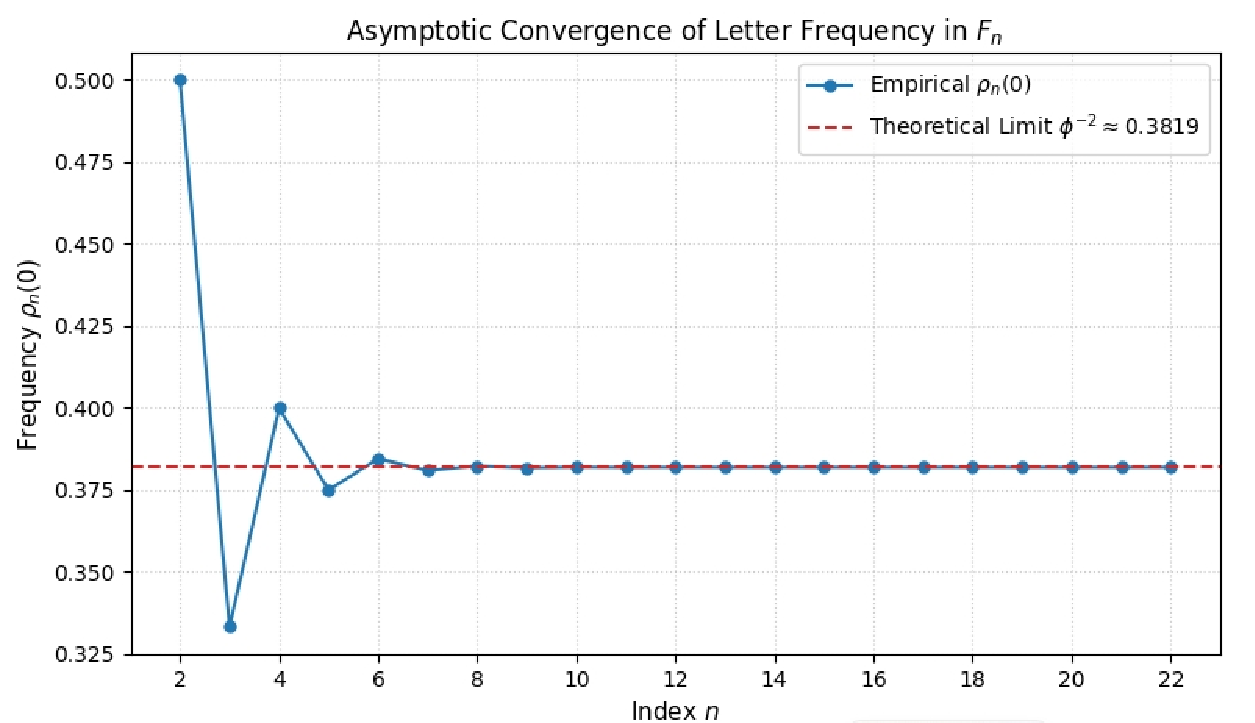
\includegraphics[width=0.99\linewidth]{figfib_conv.pdf}
	\caption{Частота буквы $1$ в $s_n$ сходится к $1/\varphi^2$ (затухающие колебания).}
	\label{fib_conv}
\end{figure}

Для любого фактора $w$ слова $\mathbf f$ длины $m$ предложение~\ref{prop:balance} даёт $|w|_1\in\{\lfloor m/\varphi^2\rfloor,\lceil m/\varphi^2\rceil\}$, так что локальные колебания плотности не превосходят $1/m$;
сравнение префиксов длин $10$ и $100$ на рис.~\ref{fig:density_comparison} иллюстрирует это.

\begin{figure}[H]
	\centering
	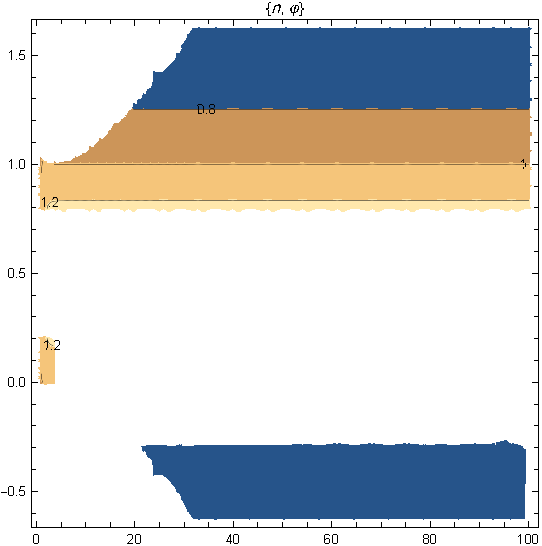
\includegraphics[width=0.5\linewidth]{Duaad8.pdf}
	\caption{Плотность буквы $1$ в префиксах длин $10$ и $100$ слова Фибоначчи.}
	\label{fig:density_comparison}
\end{figure}
%-----------------------------------------------
\begin{remark}[Взвешенные плотности]
	Если каждой букве $c$ приписана степень принадлежности $\mu(c)\in[0,1]$, то взвешенная плотность $\mathrm{FD}_c(s_n)=\mu(c)\,\mathscr D(c,s_n)$ стремится к $\mu(0)/\varphi$ при $c=0$ и к $\mu(1)/\varphi^2$ при $c=1$.
	Это лишь масштабирование классических плотностей из теоремы~\ref{mainre}; для постоянных степеней принадлежности никакого нового явления не возникает.
\end{remark}
%-----------------------------------------
\subsection{Практические приложения слова Фибоначчи}~\label{sec3.7.2}

Мы лишь кратко, без доказательств, рассматриваем два классических контекста, в которых используются доказанные выше свойства; в данной диссертации они далее не развиваются.

\begin{itemize}
	\item \textbf{Квазикристаллы.} Слово Фибоначчи является стандартной одномерной моделью квазикристалла: буквы интерпретируются как два типа связей (короткая и длинная), расположенных в цепочку в соответствии с $\mathbf f$ (Конмото--Каданов--Тан; Остлунд и др.~\cite{KKT,Ostlund}). Частоты букв, связанные с золотым сечением (теорема~\ref{mainre}), являются относительными частотами двух типов связей, а свойство сбалансированности (предложение~\ref{prop:balance}) означает, что плотность длинных связей в любом окне длины $m$ отклоняется от $1/\varphi^{2}$ менее чем на $1/m$, хотя цепочка не является периодической.
	
	\item \textbf{Кодирование.} Кодирование целых чисел по Фибоначчи, основанное на представлении Цекендорфа, является классическим универсальным кодом (Апостолико--Френкель~\cite{ApostolicoFraenkel}); в нём используются числа Фибоначчи, а не слово Фибоначчи. Само слово является стандартным примером последовательности с линейной сложностью факторов $p(n)=n+1$ и заданными частотами букв, поэтому оно используется как тестовая последовательность при изучении сжатия и повторов в строках (см.~\cite{Crochemore}).
\end{itemize}
\begin{definition}[Символико-решёточная метрика]\label{sec:dSL}
	Пусть $A$ --- конечный алфавит, $(L,\|\cdot\|)$ --- банахово пространство и $\zeta:A\to L$ --- инъективное отображение.
	Для $x,y\in A^{\mathbb Z}$ положим \begin{equation}\label{SymboliclatticeMetri} d_{SL}(x,y)=\sum_{i\in\mathbb Z}2^{-|i|}\min\{1,\|\zeta(x_i)-\zeta(y_i)\|\}, \end{equation} и $\Phi(x)=\sum_{i\in\mathbb Z}2^{-|i|}\zeta(x_i)\in L$ (абсолютно сходящийся ряд).
\end{definition}

\begin{proposition}\label{propositionn1}
	(i) $d_{SL}$ является метрикой на $A^{\mathbb Z}$, порождающей топологию произведения; следовательно, каждый подсдвиг $X\subseteq A^{\mathbb Z}$ компактен, в частности полон, относительно $d_{SL}$.
	(ii) $\|\Phi(x)-\Phi(y)\|\le\max\{1,D\}\,d_{SL}(x,y)$, где $D=\max_{a,b\in A}\|\zeta(a)-\zeta(b)\|$. В частности, $\Phi$ является $1$-липшицевым отображением, если $D\le1$.
\end{proposition}
\begin{proof}
	(i) $\min\{1,\|\cdot\|\}$ является метрикой на $\zeta(A)$, поэтому $d_{SL}$ удовлетворяет симметричности и неравенству треугольника; из $d_{SL}(x,y)=0$ следует $\zeta(x_i)=\zeta(y_i)$ для всех $i$, следовательно, $x=y$ в силу инъективности.
	Пусть $\delta_0=\min_{a\ne b}\min\{1,\|\zeta(a)-\zeta(b)\|\}>0$. Если $x_i=y_i$ при $|i|\le r$, то $d_{SL}(x,y)\le\sum_{|i|>r}2^{-|i|}=2^{1-r}$;
	если $x_i\ne y_i$ для некоторого $|i|\le r$, то $d_{SL}(x,y)\ge2^{-r}\delta_0$. Таким образом, $d_{SL}$ и метрика произведения имеют одни и те же сходящиеся последовательности, и $A^{\mathbb Z}$ компактно.
	(ii) $\|\Phi(x)-\Phi(y)\|\le\sum_i2^{-|i|}\|\zeta(x_i)-\zeta(y_i)\|$, и для каждого $i$ либо $\|\zeta(x_i)-\zeta(y_i)\|\le1$ (тогда оно равно минимуму), либо оно лежит в $(1,D]$, и минимум равен $1$,
	так что $\|\zeta(x_i)-\zeta(y_i)\|\le\max\{1,D\}\min\{1,\|\zeta(x_i)-\zeta(y_i)\|\}$.
\end{proof}	
%-------------------------------------------------
\section{Новые результаты о конструкциях слов}~\label{sec3.8}

В этом разделе развиваются новые конструкции бесконечных слов и исследуются их комбинаторные свойства с акцентом на избегание паттернов и сложность. Основная цель --- выявить богатую структуру, которую могут порождать простые итеративные правила, опираясь на основополагающие работы 
Туэ~\cite{Thue} и последующую теорию, изложенную в~\cite{Lothaire2002, Allouche}.    
%----------------------------------------------
\subsection{Сильно \texorpdfstring{$(k,\delta)$}{(k,delta)}-свободные слова посредством морфизмов циклического сдвига}

Мы вводим форму избегания паттернов, в которой перестановка алфавита вплетена в условие повторения.
Родственные понятия (псевдостепени $u\,\theta(u)\,\theta^2(u)\cdots$ для инволюции $\theta$) встречаются в литературе; приведённая ниже версия использует
перестановку $\delta$ алфавита, применяемую побуквенно.

\begin{definition}[$\delta$-скрученное слово]\label{def:twisted_word}
	Пусть $A$ --- конечный алфавит и $\delta: A \to A$ --- перестановка. Для слова $w = a_1 a_2 \dots a_n \in A^*$ его $\delta$-скрученная форма $w^{(\delta)}$ определяется применением $\delta$ побуквенно:
	\begin{equation}
		w^{(\delta)} := \delta(a_1)\, \delta(a_2) \cdots \delta(a_n).
	\end{equation}
\end{definition}

\begin{definition}[Сильный $(k, \delta)$-повтор]\label{def:strong_repetition}
	Слово $U \in A^*$ является сильным $(k, \delta)$-повтором, если оно допускает разложение $U = X_0 X_1 \cdots X_{k-1}$, в котором каждый блок имеет одну и ту же длину $|X_i| = m \ge 1$ и удовлетворяет условию
	\begin{equation}
		X_i = X_0^{(\delta^i)} \quad \text{для каждого } i,
	\end{equation}
	где $\delta^0$ --- тождественная перестановка, а $\delta^i$ обозначает $i$-ю итерацию $\delta$. Слово $W$ является сильно $(k, \delta)$-свободным, если никакой фактор слова $W$ не является сильным $(k, \delta)$-повторением.
\end{definition}

\begin{remark}
	Если $\delta$ --- тождественная перестановка, то сильное $(k,\mathrm{id})$-повторение является обычной $k$-й степенью $X_0^k$, так что сильная $(k,\mathrm{id})$-свобода есть классическая свобода от $k$-х степеней.
\end{remark}

\begin{example}
	Пусть $A = \{a, b, c\}$ и пусть $\delta$ --- циклическая перестановка $a \mapsto b \mapsto c \mapsto a$. Для $X_0 = ab$ получаем
	$X_0^{(\delta)} = bc$ и $X_0^{(\delta^2)} = ca$, так что $U = (ab)(bc)(ca)$ является сильным $(3,\delta)$-повторением с длиной блока $m=2$.
\end{example}

\begin{definition}[Морфизм циклического сдвига $\xi_{A, \sigma}$]\label{def:psiAsigma}
	Пусть $A$ --- конечный алфавит размера $N \ge 2$ и пусть $\sigma: A \to A$ --- перестановка, состоящая из одного цикла длины $N$.
	Определим $2$-равномерный морфизм $\xi_{A, \sigma}(a) = a\sigma(a)$ для $a \in A$. Для $a_0\in A$ пусть
	\begin{equation}
		W_{A, \sigma, a_0} = \lim_{n \to \infty} \xi_{A, \sigma}^n(a_0),
	\end{equation}
	неподвижная точка морфизма $\xi_{A,\sigma}$, начинающаяся с $a_0$ (она существует, поскольку $\xi_{A,\sigma}(a_0)=a_0\sigma(a_0)$).
\end{definition}

Пусть $s_2(n)$ обозначает число единиц в двоичной записи числа $n$, а $\nu_2(n)$ --- показатель степени числа $2$ в $n\ge1$.
Запишем $W=W_{A,\sigma,a_0}=W[0]W[1]W[2]\cdots$.

\begin{proposition}\label{prop:gTM}
	$W[n]=\sigma^{\,s_2(n)}(a_0)$ для каждого $n\ge0$. Следовательно, отождествляя $\sigma^t(a_0)$ с $t\in\mathbb Z/N\mathbb Z$,
	$W[n]=s_2(n) \bmod N$: слово $W$ является обобщённым словом Туэ--Морса (при $N=2$ --- словом Туэ--Морса)~\cite{Allouche}.
\end{proposition}
\begin{proof}
	Поскольку $\xi_{A,\sigma}(W)=W$ и $\xi_{A,\sigma}(a)=a\sigma(a)$, имеем $W[2n]=W[n]$ и $W[2n+1]=\sigma(W[n])$.
	Индукция по $n$: $W[0]=a_0$; $W[2n]=\sigma^{s_2(n)}(a_0)=\sigma^{s_2(2n)}(a_0)$ и
	$W[2n+1]=\sigma^{s_2(n)+1}(a_0)=\sigma^{s_2(2n+1)}(a_0)$.
\end{proof}

Для $m\ge1$ положим $c_m(n)=s_2(n+m)-s_2(n)$.

\begin{lemma}\label{lem:arith}
	Пусть $\delta=\sigma^j$. Фактор $U=X_0X_1X_2$ слова $W$ с $|X_0|=m$, начинающийся с позиции $i$, является сильным $(3,\delta)$-повторением
	тогда и только тогда, когда $c_m(n)\equiv j \pmod N$ для всех $n$ таких, что $i\le n<i+2m$.
\end{lemma}
\begin{proof}
	$X_1=\delta(X_0)$ означает, что $W[n+m]=\sigma^j(W[n])$ при $i\le n<i+m$, т.е.\ $s_2(n+m)\equiv s_2(n)+j$ (так как $\sigma$ имеет порядок $N$ на $A$);
	$X_2=\delta(X_1)$ означает то же самое при $i+m\le n<i+2m$.
\end{proof}

\begin{lemma}\label{lem:half}
	(a) $c_{2m}(2k)=c_m(k)$. (b) $c_m(n+1)-c_m(n)=\nu_2(n+1)-\nu_2(n+m+1)$.
	Следовательно, если $c_{2m}\equiv j$ на $2\cdot 2m$ последовательных целых числах, то $c_m\equiv j$ на $2m$ последовательных целых числах.
\end{lemma}
\begin{proof}
	(a) $s_2(2k+2m)=s_2(k+m)$ и $s_2(2k)=s_2(k)$. (b) Прибавление $1$ к $x$ превращает его завершающий блок из $\nu_2(x+1)$ единиц в нули, а один $0$ --- в $1$,
	так что $s_2(x+1)=s_2(x)+1-\nu_2(x+1)$; вычтем формулы для $x=n+m$ и $x=n$. Наконец, среди $4m$ последовательных целых чисел ровно $2m$ чётных, $n=2k$,
	и они соответствуют $2m$ последовательным значениям $k$; применим (a).
\end{proof}

\begin{lemma}\label{lem:odd}
	Если $c_m\equiv j \pmod N$ на $2m$ последовательных целых числах $[i,i+2m)$, где $m$ нечётно, то $m=1$ и $j\equiv1\pmod N$.
\end{lemma}
\begin{proof}
	$m=1$: среди двух последовательных целых чисел $n,n+1$ одно из $n+1,n+2$ нечётно, и $c_1(n)=1-\nu_2(n+1)$ равно $1$ при этом $n$; следовательно, $j\equiv1$.
	Пусть $m\ge3$ нечётно. По лемме~\ref{lem:half}(b), $\nu_2(x)\equiv\nu_2(x+m)\pmod N$ для $2m-1\ge5$ последовательных целых чисел $x=n+1$, $n\in[i,i+2m-2]$.
	Такой диапазон содержит два нечётных числа $x$ и $x+2$. Для нечётного $x$ имеем $\nu_2(x)=0$, а $x+m$ чётно, поэтому $\nu_2(x+m)\ge1$ и $\nu_2(x+m)\equiv0\pmod N$, следовательно, $\nu_2(x+m)\ge N\ge2$.
	Таким образом, и $x+m$, и $x+m+2$ делятся на $4$, что невозможно.
\end{proof}

\begin{theorem}[Свойство избегания для $W_{A, \sigma, a_0}$]\label{avoidance}
	Пусть $N\ge2$, $\sigma$ --- циклическая перестановка множества $A$ ($|A|=N$), и $\delta=\sigma^j$, где $j\in\mathbb Z$.
	Тогда $W_{A,\sigma,a_0}$ является сильно $(3,\delta)$-свободным тогда и только тогда, когда $j\not\equiv1\pmod N$.
\end{theorem}

\begin{proof}
	Предположим, что $W$ содержит сильное $(3,\delta)$-повторение с длиной блока $m=2^e o$, $o$ нечётно. Применяя лемму~\ref{lem:half} $e$ раз, получаем $c_o\equiv j$ на $2o$ последовательных целых числах.
	По лемме~\ref{lem:odd}, $o=1$ и $j\equiv1$. Таким образом, если $j\not\equiv1\pmod N$, то $W$ является сильно $(3,\delta)$-свободным.
	
	Обратно, пусть $j\equiv1\pmod N$ (можно взять $j=1$), $i=2^N-2$. Тогда $c_1(i)=1-\nu_2(2^N-1)=1$ и $c_1(i+1)=1-\nu_2(2^N)=1-N\equiv1\pmod N$, так что по лемме~\ref{lem:arith}
	фактор $W[i]W[i+1]W[i+2]=a\,\sigma(a)\,\sigma^2(a)$, $a=\sigma^{N-1}(a_0)$, является сильным $(3,\sigma)$-повторением.
\end{proof}

\begin{remark}
	При $j\equiv1\pmod N$ сильные $(3,\delta)$-повторы встречаются (доказательство выше). При $j\not\equiv1$ компьютерный поиск ($N=3,4,5,6$, длины блоков $m<400$, на первых $10^5$ буквах слова $W$) не обнаружил повторов, что согласуется с теоремой; при $j\equiv1$ он обнаружил повторения в точности для длин блоков $m=2^e$, $e=0,1,\dots,8$ (то есть $m=1,2,4,\dots,256$, все степени числа $2$ меньше $400$).
\end{remark}


\begin{observation}[Факторная сложность; сопоставление с известным результатом]
	Пусть $p(k)$ --- число факторов длины $k$ слова $W_{A,\sigma,a_0}$. Вычисление для $N=2,3,4$ и $k\le40$ даёт $p(1)=N$, $p(2)=N^2$ и
	$p(k+1)-p(k)\in\{N(N-1),\,N^2\}$ для всех $k\le39$, причём оба значения встречаются повторно (например, $N=3$: $p(40)=303$).
	В частности, $p(k)$ не имеет вида $(N-1)k+C_N$, в отличие от слов Арну--Ози; при $N=2$ (Туэ--Морс) разности равны $2$ и $4$.
Полная функция сложности слова $s_2(n)\bmod N$ вычислена Тромпом и Шаллитом~\cite{TrompShallit1995}. Поэтому эта закономерность рассматривается как иллюстрация известного результата, а не как самостоятельная открытая задача.
\end{observation}
%--------------------------------
\subsection{\texorpdfstring{Основание $b$ и произвольное $k$: скрученный критический показатель}{Основание b и произвольное k: скрученный критический показатель}}\label{sec:twistedk}

Пусть $b\ge2$, $N\ge2$, $\sigma$ --- циклическая перестановка множества $A$, $|A|=N$. Отождествим
$\sigma^t(a_0)$ с $t\in\mathbb Z/N\mathbb Z$, так что $\sigma(t)=t+1$. Пусть
$\xi_b(t)=t\,(t+1)\cdots(t+b-1)$ и пусть $W=W^{(b)}=\xi_b^\omega(0)$. Пусть $s_b(n)$ --- сумма
цифр числа $n$ в системе счисления с основанием $b$, а $\nu_b(x)$ --- показатель степени числа $b$ в $x\ge1$ (число завершающих нулевых цифр).

\begin{proposition}\label{tw:gTM}
	$W[n]=s_b(n)\bmod N$ для всех $n\ge0$.
\end{proposition}
\begin{proof}
	Из $\xi_b(W)=W$ следует $W[bn+r]=W[n]+r$ при $0\le r<b$, а также $s_b(bn+r)=s_b(n)+r$.
	Индукция по $n$.
\end{proof}

Для $m\ge1$ положим $c_m(n)=s_b(n+m)-s_b(n)$ и $g=N/\gcd(N,b-1)$.

\begin{lemma}\label{tw:lem}
	\begin{enumerate}
		\item[(a)] Фактор $U=X_0\cdots X_{k-1}$ слова $W$, начинающийся с позиции $i$, $|X_0|=m$, является сильным
		$(k,\sigma^j)$-повторением тогда и только тогда, когда $c_m(n)\equiv j \pmod N$ для всех $n\in[i,\,i+(k-1)m)$.
		\item[(b)] $s_b(x+1)=s_b(x)+1-(b-1)\nu_b(x+1)$, следовательно,
		$c_m(n+1)-c_m(n)=-(b-1)\bigl(\nu_b(n+m+1)-\nu_b(n+1)\bigr)$.
		\item[(c)] $c_{bm}(bn+r)=c_m(n)$ при $0\le r<b$.
		\item[(d)] Для $1\le\mu\le b-1$ и $n=bq+r$ ($0\le r<b$):
		$c_\mu(n)=\mu$, если $r<b-\mu$ (``нет переноса''), и
		$c_\mu(n)=\mu-(b-1)\bigl(1+\nu_b(q+1)\bigr)$, если $r\ge b-\mu$ (``перенос'').
	\end{enumerate}
\end{lemma}
\begin{proof}
	(a) $X_t=\delta^t(X_0)$ для всех $t$ тогда и только тогда, когда $X_{t+1}=\delta(X_t)$ при $0\le t\le k-2$, т.е.\ тогда и только тогда, когда
	$W[n+m]=W[n]+j$ для $n\in[i,i+(k-1)m)$, а $W[n]=s_b(n)\bmod N$.
	(b) Прибавление $1$ превращает $\nu_b(x+1)$ завершающих цифр $b-1$ в $0$ и увеличивает следующую цифру на $1$.
	(c) $s_b(bn+r+bm)=s_b(n+m)+r$ и $s_b(bn+r)=s_b(n)+r$.
	(d) Если $r+\mu<b$, перенос не возникает. В противном случае $n+\mu=b(q+1)+(r+\mu-b)$, так что
	$c_\mu(n)=s_b(q+1)-s_b(q)+\mu-b=\mu-(b-1)(1+\nu_b(q+1))$ по (b).
\end{proof}

\begin{theorem}[скрученный критический показатель]\label{tw:main}
	Пусть $j'\in\{1,\dots,N\}$, $j'\equiv j\pmod N$.
	\begin{enumerate}
		\item[(i)] Если $N\mid b-1$ (т.е.\ $g=1$), то $W[n]=n\bmod N$ периодично и содержит сильные
		$(k,\sigma^j)$-повторы для каждого $k$ и каждого $j$.
		\item[(ii)] Если $N\nmid b-1$ (т.е.\ $g\ge2$), то $W$ содержит сильное $(k,\sigma^j)$-повторение ($k\ge2$)
		тогда и только тогда, когда
		\begin{equation}
			k\le\kappa(N,b,j):=\max\Bigl\{2,\ \Bigl\lfloor\frac{2b}{j'}\Bigr\rfloor\Bigr\}.
		\end{equation}
		В частности, $W$ является сильно $(k,\sigma^j)$-свободным тогда и только тогда, когда $k>\kappa(N,b,j)$.
	\end{enumerate}
\end{theorem}

\begin{proof}
	(i) $s_b(n)\equiv n\pmod{b-1}$, следовательно, и по модулю $N$. Тогда $c_m(n)\equiv m$; возьмём $m\equiv j\pmod N$, $m\ge1$.
	
	(ii) Пусть $g\ge2$ и $d=\gcd(N,b-1)$. Заметим, что $(b-1)t\equiv0\pmod N\iff g\mid t$.
	
	\emph{Шаг 0: $\kappa\ge2$ для каждого $j$.} Выберем $\mu\in\{1,\dots,d\}$ с $\mu\equiv j\pmod d$
	(это возможно, так как $d\le b-1$). Поскольку $d\mid\mu-j$, сравнение $(b-1)t\equiv\mu-j\pmod N$ имеет решение
	$t\ge1$. Положим $q=b^{t-1}-1$, так что $\nu_b(q+1)=t-1$. Для $\mu$ позиций $n=bq+r$, $b-\mu\le r\le b-1$,
	лемма~\ref{tw:lem}(d) даёт $c_\mu(n)=\mu-(b-1)t\equiv j$. По (a) это сильное $(2,\sigma^j)$-повторение с $m=\mu$.
	
	\emph{Шаг 1: верхняя оценка при $k\ge3$.} Пусть существует сильное $(k,\sigma^j)$-повторение с длиной блока $m=b^em'$, $b\nmid m'$.
	По лемме~\ref{tw:lem}(c), если $c_{bm''}\equiv j$ на $(k-1)bm''$ последовательных целых числах, то
	$c_{m''}\equiv j$ на $(k-1)m''$ последовательных целых числах $n/b$ ($b\mid n$ в окне).
	Повторяя, получаем, что $c_{m'}\equiv j$ на окне из $(k-1)m'$ последовательных целых чисел.
	По (b), для $(k-1)m'-1$ последовательных $x=n+1$ в нём $\nu_b(x+m')\equiv\nu_b(x)\pmod g$. Если $b\mid x$, то $b\nmid x+m'$,
	так что $\nu_b(x)\equiv0\pmod g$ при $\nu_b(x)\ge1$, следовательно, $\nu_b(x)\ge g\ge2$ и $b^2\mid x$.
	Два кратных $b$ в этом отрезке различались бы на $b$, так что оба не могут делиться на $b^2$; таким образом, отрезок
	содержит не более одного кратного $b$, откуда $(k-1)m'-1\le 2b-1$ и, поскольку $k\ge3$, $m'\le b$, так что $m':=\mu\le b-1$.
	
	Теперь окно имеет длину $(k-1)\mu\ge2\mu>\mu$, поэтому оно содержит $n$ без переноса, что даёт $j\equiv\mu\pmod N$
	(следовательно, $\mu\ge j'$). Перенос $n=bq+r$ в окне удовлетворяет условию
	$(b-1)(1+\nu_b(q+1))\equiv0\pmod N$, т.е.\ $g\mid 1+\nu_b(q+1)$, так что $\nu_b(q+1)\ge g-1\ge1$ и $b\mid q+1$.
	Позиции переноса двух блоков $q,q'$ в окне вынуждают окно содержать позиции переноса для $q,q+1$,
	и тогда $b\mid q+1$ и $b\mid q+2$: невозможно. Таким образом, окно пересекает позиции переноса не более чем одного блока, и его длина
	не превосходит $(b-\mu)+\mu+(b-\mu)=2b-\mu$. Следовательно, $k\mu\le2b$, так что $k\le 2b/\mu\le 2b/j'$.
	
	\emph{Шаг 2: существование при $k\le 2b/j'$, когда $j'\le b-1$.} Положим $\mu=j'$, $q=b^{g-1}-1$ (так что $\nu_b(q+1)=g-1$)
	и возьмём окно $n=bq,\dots,bq+(k-1)\mu-1$ длины $\le2b-\mu$.
	Оно пересекает только позиции переноса блока $q$, где
	$c_\mu(n)=\mu-(b-1)g\equiv\mu=j'\equiv j$; позиции без переноса дают $c_\mu=\mu\equiv j$. Применим (a).
	Если $j'\ge b$, то $\lfloor 2b/j'\rfloor\le2$, так что $\kappa=2$, что в точности есть шаг~0.
\end{proof}

\begin{corollary}\label{tw:cor}
	\begin{enumerate}
		\item Если $N\nmid b-1$, то $W$ не является финально периодическим.
		(Финальный период $q$ дал бы $c_q\equiv0$ на сколь угодно длинных окнах, что противоречит $\kappa(N,b,0)<\infty$.)
		\item Для $b=2$: $\kappa=4$, если $j\equiv1\pmod N$, и $\kappa=2$ в противном случае. В частности, $W_{A,\sigma,a_0}$ является
		сильно $(3,\sigma^j)$-свободным тогда и только тогда, когда $j\not\equiv1\pmod N$, что включает классический случай $j=0$ (свобода от кубов)
		и восстанавливает теорему~\ref{avoidance}.
		\item Для $N=2$, $b=2$ (Туэ--Морс): существуют сильные $(4,\sigma)$-повторы $abab$, но ни одного при $k=5$.
	\end{enumerate}
\end{corollary}

\begin{example}
	$N=b=3$: $\kappa=6,3,2$ при $j'=1,2,3$. При $j'=2$ фактор $W[24..29]=1,2,0,1,2,0$ является сильным $(3,\sigma^2)$-повторением с $m=2$
	(блоки $12,\,01,\,20$). При $j'=1$ $W[24..29]=1,2,0,1,2,0$ является сильным $(6,\sigma)$-повторением с $m=1$. Теорема не предсказывает ничего более длинного.
\end{example}
%----------------------------------
\subsection{\texorpdfstring{Динамические свойства слова $W^{(b)}$}{Динамические свойства слова W(b)}}\label{sec:dynWb}

Пусть $N\nmid b-1$ (иначе $W$ периодично, теорема~\ref{tw:main}(i)), $X_W$ --- замыкание орбиты слова $W=W^{(b)}$
относительно сдвига $S$, а $p(k)$ --- число факторов длины $k$. Поскольку $\xi_b$ коммутирует с $\tau(t)=t+1$,
\begin{equation}\label{eq:blocks}
	W[mb^k,(m+1)b^k)=\xi_b^k(W[m])=\tau^{W[m]}\xi_b^k(0)=\bigl(W[m]+s_b(i)\bigr)_{0\le i<b^k}.
\end{equation}

\begin{theorem}\label{thm:dynWb}
	\begin{enumerate}
		\item[(1)] $\xi_b$ примитивен: $\xi_b^{k}(a)$ содержит каждую букву при $k\ge N-1$.
		\item[(2)] $W$ равномерно рекуррентно; $(X_W,S)$ минимальна.
		\item[(3)] $W$ не является финально периодическим и $k+1\le p(k)<N^2bk$. Следовательно, $h_{\mathrm{top}}(X_W)=0$.
		\item[(4)] Для каждой буквы $c$, равномерно по $i$, $\bigl||W[i,i+n)|_c-n/N\bigr|=o(n)$.
		\item[(5)] $(X_W,S)$ строго эргодична; все частоты факторов существуют равномерно.
	\end{enumerate}
\end{theorem}
\begin{proof}
	(1) $s_b(i)$, $i<b^k$, принимает каждое значение из $0,\dots,k(b-1)$; при $k\ge N-1$ встречаются все вычеты по модулю $N$.
	Воспользуемся~\eqref{eq:blocks}.
	
	(2) Пусть $u$ --- фактор, $|u|\le b^k$; он пересекает не более двух выровненных блоков длины $b^k$, так что $u$ является фактором слова $\xi_b^k(vw)$ для
	фактора $vw$ длины $2$ слова $W$, который является фактором слова $\xi_b^r(0)$ для некоторого $r$. По (1), $\xi_b^{N-1}(a)\ni0$ для каждого $a$,
	так что каждый блок $\xi_b^{T}(a)$, $T=k+r+N-1$, содержит $\xi_b^k(\xi_b^r(0))\ni u$. По~\eqref{eq:blocks}, $W$ есть конкатенация таких блоков,
	так что $u$ встречается с промежутками $\le2b^{T}$. Равномерная рекуррентность эквивалентна минимальности замыкания орбиты (стандартный факт).
	
	(3) Непериодичность есть следствие~\ref{tw:cor}(1). При $k\ge2$ возьмём $b^{e-1}<k\le b^e$ (так что $b^e<bk$). Фактор длины $k$ лежит в $\xi_b^e(W[t]W[t+1])$
	со смещением $<b^e$, так что $p(k)\le N^2b^e<N^2bk$. Теорема Морса--Хедлунда даёт $p(k)\ge k+1$.
	
	(4) Пусть $\omega=e^{2\pi\mathrm i/N}$. Из $\sum_{i<b^k}z^{s_b(i)}=(1+z+\dots+z^{b-1})^k$ и фильтра корней из единицы
	\begin{equation}
		\#\{i<b^k:s_b(i)\equiv r\}=\frac{b^k}N+E,\qquad |E|\le\beta^k,\quad
		\beta=\max_{1\le\ell<N}\Bigl|\sum_{d=0}^{b-1}\omega^{\ell d}\Bigr|<b
	\end{equation}
	($\beta<b$ в силу строгости неравенства треугольника, поскольку $\omega^\ell\ne1$). По~\eqref{eq:blocks} каждый выровненный блок длины $b^k$ содержит
	каждую букву $b^k/N+E'$ раз, $|E'|\le\beta^k$, независимо от блока. Выберем $b^k\le\sqrt n<b^{k+1}$.
	Окно длины $n$ состоит не более чем из $n/b^k$ выровненных блоков и не более чем из $2b^k$ граничных позиций, так что
	отклонение от $n/N$ не превосходит $n(\beta/b)^k+2b^k+2b^k/N=o(n)$.
	
	(5) По (1), $\xi_b$ является примитивной подстановкой, а $W$ --- её неподвижной точкой; по теореме Мишеля (см. Кеффелек~\cite{Queffelec}, гл.~5)
	её подсдвиг строго эргодичен, что эквивалентно существованию равномерной частоты у каждого фактора.
\end{proof}

\begin{corollary}
	Каждый $x\in X_W$ является сильно $(k,\sigma^j)$-свободным при $k>\kappa(N,b,j)$.
\end{corollary}
\begin{proof}
	В силу минимальности (2) язык $x$ совпадает с языком $W$; применим теорему~\ref{tw:main}.
\end{proof}

\begin{remark}[интерпретация через коцикл]
	По лемме~\ref{tw:lem}(b), $n\mapsto s_b(n+1)-s_b(n)=1-(b-1)\nu_b(n+1)$ есть функция со значениями в $\mathbb Z/N$ от точки
	$n$ $b$-адического одометра, так что $W$ есть кодирование $\mathbb Z/N$-косого произведения над одометром. Сильное
	$(k,\sigma^j)$-повторение есть окно, на котором суммы Биркгофа $c_m$ этой функции за $m$ шагов постоянно равны $j$.
	Именно поэтому задача об избегании сводится к арифметике $\nu_b$.
\end{remark}

\begin{proposition}[сдвиг в символико-решёточной метрике]\label{prop:dSLshift}
	Для $d_{SL}$ из определения~\ref{sec:dSL} выполняется $d_{SL}(Sx,Sy)\le2\,d_{SL}(x,y)$ на $A^{\mathbb Z}$.
\end{proposition}
\begin{proof}
	При $\delta_i=\min\{1,\|\zeta(x_i)-\zeta(y_i)\|\}$:
	$d_{SL}(Sx,Sy)=\sum_j2^{-|j-1|}\delta_j\le2\sum_j2^{-|j|}\delta_j$, поскольку $|j-1|\ge|j|-1$.
\end{proof}

\begin{remark}
	Для односторонних подсдвигов $X\subseteq A^{\mathbb N}$ положим
	\begin{equation}
		d_{SL}(x,y)=\sum_{i\ge0}2^{-i}\min\{1,\|\zeta(x_i)-\zeta(y_i)\|\}.
	\end{equation}
	Тогда
	\begin{equation}
		d_{SL}(Sx,Sy)=\sum_{j\ge1}2^{-(j-1)}\delta_j\le2\,d_{SL}(x,y)
	\end{equation}
	тем же вычислением, так что предложение~\ref{prop:dSLshift} справедливо для подсдвига $X_W$ из теоремы~\ref{thm:dynWb}.
\end{remark}
%---------------------------------------

\subsection{Обсуждение и дальнейшая работа}

Теорема~\ref{avoidance} и её обобщение, теорема~\ref{tw:main}, решают вопрос о сильной $(k,\sigma^j)$-свободе для всех $k\ge2$, всех $j$ и каждого основания $b$ для слов $W^{(b)}$; минимальность, нулевая топологическая энтропия и строгая эргодичность соответствующего подсдвига доказаны в теореме~\ref{thm:dynWb}. Следующие вопросы остаются открытыми:
\begin{itemize}
	\item сильная $(k,\delta)$-свобода для перестановок $\delta$, не являющихся степенями $\sigma$;
	\item исследование сложности языков для более общих перестановочных ограничений; классическая сложность $s_2(n)\bmod N$ при этом уже известна~\cite{TrompShallit1995};
	\item алгоритмы, обнаруживающие сильные $(k,\delta)$-повторы в конечных словах.
\end{itemize}
%%%%%%%%%%%%%%%%%%%%%%%%%%%%%%%%%%%%%%%%%%%%%%%%
\chapter{Практические приложения, математические головоломки и образование}~\label{sec4}

Эта глава имеет образовательную направленность. В разделе~\ref{sec4.1} обсуждается роль математических головоломок в обучении. В разделе~\ref{sec4.2} решается задача о минимальном разрезании полимино, которая может быть использована как учебное задание. В разделе~\ref{sec4.3} сообщается о квазиэкспериментальном исследовании с учениками шестого класса в Алеппо; его результаты носят предварительный характер, поскольку группы различались на исходном уровне, а скорректированная разность статистически не значима.
%-------------------------------------
\section{Роль математических народных головоломок в развитии математического мышления и навыков решения задач}~\label{sec4.1}

На протяжении веков математические народные головоломки служили педагогическими инструментами для школьников во многих культурах. В XXI веке эти головоломки продолжают увлекать учащихся по всему миру, предоставляя неформальный, но богатый контекст, в котором обучающиеся могут исследовать геометрические фигуры, площадь, периметр, симметрию, углы, закономерности, отношения и мультипликативное мышление. Взрослые, наблюдающие за детьми, часто упускают эти моменты математического исследования, воспринимая деятельность как простую игру, а не как подлинное обучение. Однако в школьных условиях головоломки, представленные как задачи-вызовы или соревнования, показали измеримое влияние на учебную успеваемость.

Математические головоломки служат универсальным обучающим инструментом для разных возрастных групп. Их сила заключается в сочетании увлекательности с интеллектуальной требовательностью: хорошо поставленная головоломка привлекает учащихся любопытством, незаметно требуя от них тщательно рассуждать, проверять идеи и пересматривать свои мысли.

Из этого следует несколько педагогических преимуществ. Во-первых, головоломки приучают учащихся анализировать задачу, прежде чем действовать, взвешивать конкурирующие подходы и строить аргументацию, а не воспроизводить заученную процедуру. 
Столкновение с задачей, не поддающейся рутинным методам, подталкивает учащихся к поиску структуры, которую они в ином случае могли бы не заметить.

Во-вторых, итеративный характер решения головоломок формирует настойчивость. Учащийся, проходящий через повторные неудачные попытки перед достижением решения, узнаёт то, чему не могут научить одни лишь правильные ответы: что замешательство является нормальным этапом математической работы, а не сигналом остановиться. Это определяет, как учащиеся относятся к трудностям в долгосрочной перспективе.

В-третьих, когда головоломки решаются совместно, они создают условия для подлинного математического диалога. Учащимся приходится формулировать свои рассуждения, отвечать на возражения и согласовывать конкурирующие стратегии --- привычки мышления, которые переносятся далеко за пределы самой головоломки.

Пожалуй, самое важное: головоломки меняют представление о том, какова математика на ощупь. Предмет, который часто воспринимается как последовательность процедур для запоминания, может благодаря одной удачно выбранной задаче раскрыться как открытый, удивительный и достойный исследования ради него самого. Учащиеся, встречающиеся с математикой таким образом, склонны сохранять иную ориентацию по отношению к ней.

С учётом этих соображений следующая подборка головоломок составлена для того, чтобы бросать вызов, увлекать и побуждать к устойчивому математическому мышлению.
%------------------------------------
\subsection{Исторический контекст и образовательная ценность математических народных головоломок}~\label{sec4.1.1}

Математические народные головоломки на протяжении веков служили педагогическими инструментами в разных культурах, отражая исторические и образовательные контексты, в которых они возникли. В отличие от задач, придуманных исключительно для развлечения, многие классические народные головоломки моделировали повседневные проблемы, такие как вычисление вместимости сосудов или суммирование связок палочек, имевшие практическое значение в повседневной жизни~\cite{Picciotto}. Профессиональные математики исторически отдавали предпочтение задачам, поддающимся геометрическим или аналитическим методам, тогда как народные математики, как правило, занимались счётом и простой арифметикой. Решая такие головоломки, учащиеся сталкиваются со свойствами чисел и объектов, часто игнорируемыми в стандартных учебных программах, и поощряются к критическому мышлению, обобщению и даже к придумыванию собственных головоломок~\cite{Danesi, Iortser}.

Образовательная ценность математических головоломок хорошо установлена. 
Когда учащиеся работают с головоломками, они не просто усваивают конкретное понятие: они применяют классные знания к сравнительно сложным задачам, представленным в виде игр или вызовов, развивая тем самым логические навыки, переносимые на широкий круг контекстов. Головоломки способствуют критическому мышлению и логическому рассуждению, воспитывают упорство и стойкость, а при совместном решении поддерживают общение и конструктивную аргументацию. Они также помогают изменить восприятие математики с абстрактного и скучного предмета на увлекательный и интеллектуально стимулирующий~\cite{Boaler}. 
В сочетании с цифровыми инструментами, такими как интерактивные доски и онлайн-репозитории, обучение на основе головоломок способствует повышению вовлечённости, концептуального понимания и 
успеваемости~\cite{Pramestika, Ahdhianto}.
%---------------------------------------------
\subsection{Типы геометрических головоломок}~\label{sec4.1.2}

Геометрические головоломки развивают пространственное мышление, зрительные навыки и понимание геометрических принципов. Четыре основных типа особенно ценны в образовательных условиях.

\textbf{Танграмы} --- древние китайские головоломки, состоящие из семи плоских частей --- пяти треугольников, одного квадрата и одного параллелограмма --- которые можно расположить так, чтобы получить различные фигуры (рис.~\ref{fign1}). Они дают практический опыт работы с геометрическими преобразованиями, такими как поворот, симметрия и конгруэнтность, одновременно развивая пространственное мышление, мелкую моторику и настойчивость~\cite{Boaler}.

\begin{figure}[H]
	\centering
	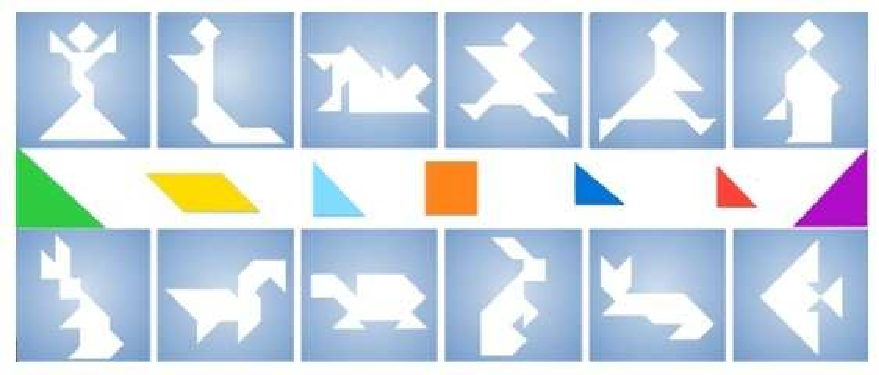
\includegraphics[width=\textwidth]{firstimg.pdf}
	\caption{Семь частей набора танграма.}\label{fign1}
\end{figure}

\textbf{Геометрические пазлы и головоломки на разрезание} требуют от учащихся разбиения и повторной сборки фигур, закрепляя понятия сохранения площади, конгруэнтности и замощения (рис.~\ref{fign2}). Пентамино --- двенадцать уникальных фигур, каждая из которых составлена из пяти единичных квадратов --- представляют собой хорошо известное семейство таких головоломок, естественно связанное с идеями площади, симметрии и комбинаторного перечисления~\cite{Puig}.

\begin{figure}[H]
	\centering
	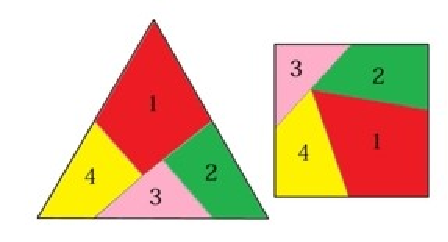
\includegraphics[width=10cm, height=5cm]{dua2.pdf}
	\caption{Примеры геометрических головоломок на разрезание.}\label{fign2}
\end{figure}

\textbf{Блоки-паттерны} --- наборы красочных геометрических фигур, включая шестиугольники, треугольники, квадраты, трапеции и ромбы --- позволяют учащимся создавать узоры и композиции, закрепляющие симметрию, соотношения между углами и пространственную структуру, одновременно поощряя творчество и практическое исследование.
%-------------------------------------
\subsection{Цифровые и геймифицированные подходы}~\label{sec4.1.3}

Интеграция технологий в математическое образование может существенно повысить вовлечённость учащихся и результаты обучения. Показано, что геймифицированные методы обучения, включающие уровни, задания, значки и системы вознаграждения, повышают мотивацию и делают обучение интерактивным и целеориентированным~\cite{Luo, Cal}. Технология дополненной реальности (AR) предлагает взаимодополняющий подход, позволяя учащимся виртуально манипулировать геометрическими объектами, такими как разрезания и трёхмерные фигуры, что поддерживает более глубокое концептуальное понимание и улучшенное пространственное мышление~\cite{Flores}. Эти цифровые инструменты наиболее эффективны в сочетании с практическими классными занятиями: например, поиск фигур, закрепляющий геометрическое распознавание, задания по проектированию зданий, связывающие геометрию с контекстами реального мира~\cite{Puig}, и проекты по геометрическому искусству, объединяющие математическое и творческое мышление.
%---------------------------------------------------
\subsection{Логические, вероятностные и комбинаторные головоломки}~\label{sec4.1.4}

Логические головоломки требуют дедуктивного рассуждения и систематического мышления, а не воспроизведения фактов. Классические примеры, такие как задачи о переправе через реку и головоломки о рыцарях и лжецах, дают превосходный контекст для упражнения в доказательной аргументации~\cite{Rakshit}. Алгебраические головоломки, включая головоломки с уравнениями, такие как магические квадраты, и головоломки с функциями, включающие композиции $f(g(x))$, развивают математическое рассуждение и беглость в алгебре, побуждая обучающихся интерпретировать структуру, а не просто применять процедуры.

Две вероятностные головоломки заслуживают особого внимания благодаря своей педагогической силе. \textbf{Задача Монти Холла} демонстрирует, что постоянная смена дверей после того, как ведущий открывает дверь с козой, увеличивает вероятность выигрыша с $1/3$ до $2/3$, как показано на дереве решений на рис.~\ref{fign3}. Этот поразительный результат делает её мощным учебным примером для условной вероятности и байесовского рассуждения.

\begin{figure}[H]
	\centering
	\resizebox{0.96\linewidth}{!}{%
\begin{tikzpicture}[node distance=20mm and 26mm,
		box/.style={rectangle, draw, minimum size=8mm, text centered},
		lab/.style={font=\footnotesize, align=right},
		el/.style={midway, fill=white, inner sep=1.5pt, font=\small},
		>=latex]
		\node (start) {старт};
		\node[box, below left=of start] (D1) {D1};
		\node[box, below=of start] (D2) {D2};
		\node[box, below right=of start] (D3) {D3};
		\node[box, below left=of D1] (D2b) {D2};
		\node[box, below=of D1] (D3b) {D3};
		\node[box, below=of D2] (D3c) {D3};
		\node[box, below=of D3] (D2c) {D2};
		\draw[->] (start) -- node[el] {1/3} (D1);
		\draw[->] (start) -- node[el] {1/3} (D2);
		\draw[->] (start) -- node[el] {1/3} (D3);
		\draw[->] (D1) -- node[el] {1/2} (D2b);
		\draw[->] (D1) -- node[el] {1/2} (D3b);
		\draw[->] (D2) -- node[el] {1} (D3c);
		\draw[->] (D3) -- node[el] {1} (D2c);
		\node[below=3mm, red] (p1) at (D2b.south) {1/6};
		\node[below=3mm, red] at (D3b.south) {1/6};
		\node[below=3mm, red] at (D3c.south) {1/3};
		\node[below=3mm, red] at (D2c.south) {1/3};
		\node[below=11mm] (s1) at (D2b.south) {МАШИНА};
		\node[below=11mm] at (D3b.south) {МАШИНА};
		\node[below=11mm] at (D3c.south) {КОЗА};
		\node[below=11mm] at (D2c.south) {КОЗА};
		\node[below=19mm] (w1) at (D2b.south) {КОЗА};
		\node[below=19mm] at (D3b.south) {КОЗА};
		\node[below=19mm] at (D3c.south) {МАШИНА};
		\node[below=19mm] at (D2c.south) {МАШИНА};
		\node[lab, left=1mm of D1] {Машина за\\дверью:};
		\node[lab, left=1mm of D2b] {Ведущий открывает\\дверь:};
		\node[lab, left=1mm of p1] {Вер.:};
		\node[lab, left=1mm of s1] {Остаться:};
		\node[lab, left=1mm of w1] {Сменить:};
	\end{tikzpicture}
}
	\caption{Дерево решений, иллюстрирующее задачу Монти Холла.}\label{fign3}
\end{figure}

\textbf{Парадокс дней рождения} показывает, что достаточно лишь 23 человек, чтобы вероятность совпадения дней рождения превысила $50\%$. Дополнительная вероятность того, что никакие два человека в группе из $n$ человек не имеют общего дня рождения, равна
\begin{equation}
	\bar{p}(n) = \frac{365!}{365^n(365-n)!},
\end{equation}
откуда $p(23) = 1 - \bar{p}(23) \approx 0.507$~\cite{Feliciano}. 
Оба парадокса наглядно иллюстрируют, как интуиция может вводить в заблуждение при вероятностных рассуждениях, и находят практическое применение в 
криптографии посредством анализа коллизий хеш-функций~\cite{Bevan, Alvarado}.

Комбинаторные головоломки сосредоточены на расположении и выборе дискретных элементов. Шахматные задачи, такие как задача о восьми ферзях, обход конём и задачи о доминировании, развивают пространственное восприятие и стратегическое планирование, естественно связываясь с теорией графов и оптимизацией. Головоломки с перестановками, включая кубик Рубика, 
головоломки-пятнашки и ханойскую башню (требующую минимум $2^n - 1$ ходов для $n$ дисков), вводят экспоненциальный рост, рекурсивные определения и алгоритмическое мышление в 
доступном контексте.
%---------------------------------------------
\section{Задача о минимальном пути разрезания полимино}~\label{sec4.2}

В то время как классические головоломки на разрезание сосредоточены на перестановке частей для создания новых фигур, мы изучаем эффективность самого процесса разрезания.

\emph{Полимино} $P$ --- это связное объединение $N$ единичных квадратов целочисленной сетки. \emph{Разрез} --- это полная горизонтальная или вертикальная линия сетки
$x=c$ или $y=c$ ($c\in\mathbb Z$), применяемая ко всем текущим частям одновременно, без перемещения частей. Два квадрата из $P$ \emph{смежны}, если они имеют общую сторону;
такая общая сторона называется \emph{внутренним ребром} $P$. Пусть $\lambda(P)$ --- число линий сетки, содержащих хотя бы одно внутреннее ребро $P$.
Цель состоит в том, чтобы разделить $P$ на его $N$ единичных квадратов наименьшим числом разрезов.

\begin{theorem}\label{thm:min-dissection-path}
	Минимальное число разрезов, необходимое для разрезания полимино $P$ на его единичные квадраты, равно $\lambda(P)$. В частности, прямоугольнику $a\times b$ требуется $(a-1)+(b-1)$ разрезов.
\end{theorem}

\begin{proof}
	После применения множества $S$ линий разреза части являются компонентами связности $P$ с удалёнными линиями из $S$. Два смежных квадрата остаются в одной части
	тогда и только тогда, когда линия, содержащая их общую сторону, не принадлежит $S$ (внутренность единичной стороны лежит ровно на одной линии сетки).
	Следовательно, все квадраты разделены тогда и только тогда, когда каждое внутреннее ребро лежит на линии из $S$, т.е.\ $S$ содержит все $\lambda(P)$ линий, несущих внутреннее ребро.
	Обратно, выбор $S$, равного этим линиям, подходит: любой путь между двумя различными квадратами внутри $P$ пересекает внутреннее ребро, которое разрезано.
	Для прямоугольника $a\times b$ линиями, несущими внутренние рёбра, являются $a-1$ вертикальных и $b-1$ горизонтальных линий.
\end{proof}

\begin{remark}
	Если же каждый разрез удаляет одно единичное внутреннее ребро, то минимум равен числу внутренних рёбер, которое равно $N-1$ тогда и только тогда, когда граф смежности $P$ является деревом
	(для квадрата $2\times2$ оно равно $4$, а не $3$). Поэтому значение $N-1$ в общем случае неверно ни в одной из моделей.
\end{remark}

\begin{example}[Квадрат $2\times2$ и квадрат $3\times3$]
	Для квадрата $2\times2$ ($N=4$) достаточно линий $x=1$ и $y=1$, так что $2$ разрезов достаточно, что меньше $N-1=3$.
	Для квадрата $3\times3$ ($N=9$) достаточно $4$ разрезов, что меньше $N-1=8$.
\end{example}

\begin{itemize}
	\item \textbf{Примеры минимальных путей разрезания}
	
	Чтобы проиллюстрировать теорему~\ref{thm:min-dissection-path}, рассмотрим два простых полимино.
	
	\begin{example}[\textbf{Домино $(N=2)$}]\label{ex1}
		Домино --- это полимино, составленное из двух единичных квадратов. Теорема даёт $\lambda(P)=1$: единственное внутреннее ребро лежит на линии $x=1$, так что один разрез необходим и достаточен. Как показано на рис.~\ref{fign4}, одного прямого разреза вдоль общего ребра достаточно, чтобы разделить два квадрата.
	\end{example}
	
	\begin{figure}[H]
		\centering
		\begin{tikzpicture}[scale=.8]
			\draw [line width=2pt] (0,6)-- (0,4);
			\draw [line width=2pt] (0,4)-- (2,4);
			\draw [line width=2pt] (2,4)-- (2,6);
			\draw [line width=2pt] (2,6)-- (0,6);
			\draw [line width=2pt] (2,6)-- (4,6);
			\draw [line width=2pt] (4,6)-- (4,4);
			\draw [line width=2pt] (4,4)-- (2,4);
			\draw [line width=2pt] (0,3)-- (2,3);
			\draw [line width=2pt] (2,3)-- (2,1);
			\draw [line width=2pt] (2,1)-- (0,1);
			\draw [line width=2pt] (0,1)-- (0,3);
			\draw [line width=2pt,dash pattern=on 1pt off 1pt] (3,3)-- (3,1);
			\draw [line width=2pt] (4,3)-- (4,1);
			\draw [line width=2pt] (4,3)-- (6,3);
			\draw [line width=2pt] (6,3)-- (6,1);
			\draw [line width=2pt] (6,1)-- (4,1);
		\end{tikzpicture}
		\caption{Минимальное разрезание домино: один прямой разрез разделяет полимино $(1\times 2)$ на два единичных квадрата.}\label{fign4}
	\end{figure}
	
	\begin{example}[\textbf{L-тримино ($(N=3)$)}]\label{ex2}
		L-тримино --- это полимино, состоящее из трёх единичных квадратов, расположенных в форме буквы <<L>>. Здесь $\lambda(P)=2$: одна вертикальная и одна горизонтальная линии сетки несут внутренние рёбра, так что два разреза необходимы и достаточны. Рисунок~\ref{fign5} иллюстрирует один из подходов: первый разрез отделяет один из крайних квадратов, в результате чего получается домино, а второй разрез делит оставшиеся два квадрата.
	\end{example}
	
	\begin{figure}[H]
		\centering
		\begin{tikzpicture}[scale=.8]
			\draw [line width=2pt] (0,6)-- (0,4);
			\draw [line width=2pt] (0,4)-- (2,4);
			\draw [line width=2pt] (2,4)-- (2,6);
			\draw [line width=2pt] (2,6)-- (0,6);
			\draw [line width=2pt] (2,6)-- (4,6);
			\draw [line width=2pt] (4,6)-- (4,4);
			\draw [line width=2pt] (4,4)-- (2,4);
			\draw [line width=2pt] (0,3)-- (2,3);
			\draw [line width=2pt] (2,3)-- (2,1);
			\draw [line width=2pt] (2,1)-- (0,1);
			\draw [line width=2pt] (0,1)-- (0,3);
			\draw [line width=2pt] (4,3)-- (4,1);
			\draw [line width=2pt] (4,3)-- (6,3);
			\draw [line width=2pt] (6,3)-- (6,1);
			\draw [line width=2pt] (6,1)-- (4,1);
			\draw [line width=2pt] (0,6)-- (0,8);
			\draw [line width=2pt] (0,8)-- (2,8);
			\draw [line width=2pt] (2,8)-- (2,6);
			\draw [line width=2pt] (7,3)-- (9,3);
			\draw [line width=2pt] (9,3)-- (9,1);
			\draw [line width=2pt] (9,1)-- (7,1);
			\draw [line width=2pt] (7,1)-- (7,3);
		\end{tikzpicture}
		\caption{Минимальное разрезание L-тримино: два прямых разреза разделяют три единичных квадрата.}\label{fign5}
	\end{figure}
	
	Эти примеры дают конкретные примеры минимальных путей разрезания и наглядно подтверждают теорему~\ref{thm:min-dissection-path}.
\end{itemize}

\begin{itemize}
	\item \textbf{Значимость и адаптация для использования в классе}
	Задача о минимальном пути разрезания полимино, хотя и основана на теоретической геометрии и комбинаторике, имеет значительную образовательную ценность. Её можно адаптировать для различных уровней обучения --- от элементарных исследований площади и периметра до более продвинутых обсуждений графов, рекурсии и оптимизации. Её практический характер в сочетании с ясной лежащей в основе математической структурой делает её увлекательным контекстом для развития критического мышления, пространственного рассуждения и навыков решения задач у учащихся. 
\end{itemize}
%---------------------------------------------
\subsection{Педагогические преимущества}~\label{sec4.2.1}

\begin{enumerate}
	\item \textbf{Концептуальное понимание площади и разбиения.}
	На фундаментальном уровне разрезание полимино на единичные квадраты закрепляет понятие площади как суммы дискретных единиц. Учащиеся могут наглядно и кинестетически осознать, что полимино площади $(N)$ составлено из $(N)$ единичных квадратов, которые в принципе можно разделить~\cite{Boaler}. Это укрепляет связи между символическими формулами площади и конкретными представлениями на сетке. 
	
	\item \textbf{Пространственное рассуждение и визуализация.}
	Процесс определения оптимальных линий разреза требует развитого пространственного рассуждения. Учащиеся должны визуализировать, как разрез разделит фигуру и как полученные части могут быть далее разрезаны или переставлены. Такие занятия повышают их способность мысленно манипулировать двумерными объектами и формируют основные компоненты пространственного мышления~\cite{Puig}. 
	
	\item \textbf{Решение задач и оптимизация.}
	Суть задачи о минимальном пути разрезания состоит в нахождении минимального числа разрезов, что знакомит учащихся с идеей оптимизации --- поиском наиболее эффективного решения при заданных ограничениях. Обучающиеся естественным образом прибегают к методу проб и ошибок, сравнению стратегий и обоснованию того, почему данное решение оптимально, развивая тем самым прочные навыки решения задач и критическое мышление~\cite{Ahdhianto}. 
	
	\item \textbf{Введение в теорию графов и алгоритмы (продвинутые уровни).}
	Для старших или более продвинутых учащихся задача может служить доступным введением в графовое моделирование. Каждый единичный квадрат можно представить как узел, а общие границы между квадратами --- как рёбра. Процесс разрезания тогда можно интерпретировать как разделение узлов посредством разрезов, что открывает возможность обсуждения рёберных разрезов, связности и алгоритмических стратегий, а также неформальных понятий вычислительной сложности.
	
	\item \textbf{Настойчивость и стойкость.}
	Как и в случае многих содержательных головоломок, учащиеся могут не найти оптимальное решение сразу.Проработка почти удачных попыток и совершенствование приёмов способствуют упорству и стойкости, учат детей настойчиво преодолевать трудности и воспринимать ошибки как полезную обратную связь, а не как неудачу. Это способствует формированию установки на рост в арифметике.
\end{enumerate}
%----------------------------------------
\subsubsection{Классные задания и адаптации}~\label{sec4.2.2}

\begin{enumerate}
	\item \textbf{Разрезание физических полимино}
	\begin{enumerate}
		\item \textbf{Материалы.} Предложите учащимся фигуры-полимино, вырезанные из бумаги, картона или поролона. Эти фигуры должны быть нарисованы на квадратной сетке, чтобы выделить отдельные единичные квадраты.
		\item \textbf{Деятельность.} Предложите учащимся разрезать полимино на отдельные квадраты, используя как можно меньше прямолинейных разрезов. Они записывают свои разрезы и число получившихся частей после каждого шага. Эта практическая деятельность поощряет непосредственное манипулирование, исследование и выдвижение гипотез.
		\item \textbf{Обсуждение.} После выполнения задания проведите обсуждение стратегий со всем классом. Нашли ли учащиеся минимальное число разрезов, то есть число линий сетки, несущих внутреннее ребро? Почему да или почему нет? Какие фигуры было легче или труднее разрезать, и какие структурные особенности, по-видимому, имели значение?
	\end{enumerate}
	
	\item \textbf{Цифровые интерактивные инструменты}
	\begin{enumerate}
		\item \textbf{Программное обеспечение.} Используйте программы динамической геометрии или онлайн-интерактивные платформы, где учащиеся могут рисовать полимино и моделировать прямолинейные разрезы. Цифровая среда позволяет легко отменять действия, повторять попытки и автоматически отслеживать число разрезов.
		\item \textbf{Геймификация.} Реализуйте геймифицированную версию, в которой учащиеся зарабатывают баллы или значки за достижение минимального числа разрезов или за успешное разрезание более сложных полимино. Таблицы лидеров и уровни могут способствовать дружественному соревнованию и устойчивой вовлечённости~\cite{Cal}.
	\end{enumerate}
	
	\item \textbf{Дневники решения задач}
	\begin{enumerate}
		\item \textbf{Деятельность.} Попросите учащихся документировать процессы разрезания в дневнике. Они рисуют исходное полимино, зарисовывают предлагаемые разрезы и объясняют соображения, стоящие за их выбором. Эта практика способствует метапознанию и даёт учителям представление о стратегиях и заблуждениях учащихся.
	\end{enumerate}
	
	\item \textbf{Задание на проектирование полимино}
	\begin{enumerate}
		\item \textbf{Деятельность.} Предложите учащимся спроектировать полимино, которые, по их мнению, особенно <<легко>> или <<трудно>> разрезать минимальным числом разрезов. Затем они должны проверить и обосновать свои гипотезы, используя принципы задачи о минимальном пути разрезания. Эта деятельность поощряет творчество, обобщение и аргументацию~\cite{Pramestika}.
	\end{enumerate}
	
	\item \textbf{Связь с приложениями в реальном мире}
	\begin{enumerate}
		\item \textbf{Обсуждение.} Организуйте обсуждение того, как задачи оптимизации, подобные минимизации числа разрезов, возникают в реальных контекстах. Примеры включают производство (минимизация отходов материала при раскрое листов), логистику (оптимизация маршрутов или разбиение регионов) и информатику (эффективная сегментация и обработка данных). Это помогает учащимся осознать более широкую значимость математической оптимизации в повседневной жизни~\cite{Maryana}.
	\end{enumerate}
\end{enumerate}

Интегрируя задачу о минимальном пути разрезания в учебную программу посредством таких разнообразных видов деятельности, педагоги могут превратить абстрактную математическую идею в осязаемый, увлекательный и педагогически богатый учебный опыт.
%--------------New Section ----------
\section{Влияние использования народных математических головоломок на математическое мышление сирийских школьников}~\label{sec4.3}

Головоломки и игры являются древними инструментами интеллектуального вовлечения, широко рассматриваемыми как средство развития критического мышления и вовлечения учащихся в математическое исследование. В математическом образовании народные головоломки могут служить эффективным инструментом совершенствования навыков решения задач: решение головоломки требует логического рассуждения, распознавания закономерностей и способности творчески применять математические понятия. Головоломки также могут привнести элемент удовольствия в предмет, который часто воспринимается как трудный, помогая поддерживать интерес учащихся и позволяя даже испытывающим трудности школьникам постепенно участвовать в сложных заданиях~\cite{Boaler}. 

Человеческое познание основано не только на логических и аналитических процессах. Специалисты по когнитивным наукам подчёркивают роль <<выведения смысла>> в аналитическом рассуждении, и этот механизм глубоко задействован при решении головоломок. Осмысление лучше всего развивается тогда, когда уму предлагается задача, которая является сложной, приятной и вознаграждающей --- условия, которые психология описывает как благодатную почву для эффективного обучения. Головоломки предлагают именно такой ресурс для математики --- предмета, который часто рассматривается как абстрактный и оторванный от реальной жизни.

В этом разделе сообщается об эмпирическом исследовании того, как обучение на основе головоломок влияет на математическое мышление учеников шестого класса в Сирии. Система образования страны подверглась серьёзному напряжению в результате более чем тринадцати лет конфликта, и малозатратные педагогические стратегии имеют особую ценность в такой обстановке. Поэтому в исследовании изучается малозатратный подход к обучению как возможный вклад в восстановление образования.

%--------------------------------------------
\subsection*{Проблема и цель исследования}~\label{sec4.3.1}

Система образования Сирии остро нуждается в модернизации. Значительная доля учеников начальной школы испытывает трудности с математикой, отчасти потому, что преподавание в основном теоретическое, опирается на механическое заучивание и лишено практических или увлекательных компонентов~\cite{Duaa}. В данном исследовании изучается подход к обучению на основе головоломок как альтернатива, и ставятся следующие исследовательские вопросы:

\begin{enumerate}
	\item Существует ли статистически значимое различие (при $\alpha = 0.05$) в оценках математического мышления между учащимися, обучавшимися с использованием математических головоломок, и учащимися, обучавшимися традиционными методами, с учётом результатов предварительного тестирования?
	\item Существует ли статистически значимое различие (при $\alpha = 0.05$) в оценках по тесту на натуральные и целые числа между экспериментальной и контрольной группами с учётом результатов предварительного тестирования? 
\end{enumerate}

%-------------------------------------------------
\subsection*{Значимость исследования}~\label{sec4.3.2}

Данное исследование имеет три значения. Во-первых, оно посвящено математическому образованию в контексте кризиса, теме, значимость которой растёт в международном образовательном дискурсе. Во-вторых, оно сосредоточено на учениках шестого класса на критическом этапе формирования базовых математических навыков и установок и предлагает головоломки как педагогический инструмент, способный улучшить понимание и одновременно дать учителям более глубокое представление о мышлении учащихся. В-третьих, эмпирические исследования обучения на основе головоломок в арабском мире редки, поэтому данное исследование восполняет пробел в региональных исследованиях.

%---------------------------------------------------
\subsection*{Гипотезы исследования}~\label{sec4.3.3}

\begin{itemize}
	\item[$H_{01}$:] Не существует статистически значимого различия (при $\alpha = 0.05$) между экспериментальной и контрольной группами в итоговых оценках математического мышления (тест из 12 баллов), скорректированных с учётом предварительных оценок.
	\item[$H_{02}$:] Не существует статистически значимого различия (при $\alpha = 0.05$) между двумя группами в итоговых оценках по тесту на натуральные и целые числа (шкала 0--100), скорректированных с учётом предварительных оценок.
\end{itemize}

\textbf{Генеральная совокупность и выборка.} Целевая генеральная совокупность включала всех учеников шестого класса школы Our Lady of Mary School в Алеппо, Сирия (приблизительно 400 учеников).
В течение первого семестра 2024--2025 учебного года изучались два класса: экспериментальная группа (группа~B, $n=42$), обучавшаяся с использованием математических головоломок, и контрольная группа (группа~A, $n=42$), обучавшаяся традиционными методами, всего 84 ученика. 
Обе группы обучал один и тот же исследователь для обеспечения единообразия преподавания.

\textbf{Ограничения исследования.} Исследование было ограничено первыми двумя разделами учебника для шестого класса (натуральные и целые числа), проводилось в течение одного семестра в одной школе в Алеппо и использовало целые классы, поэтому план исследования является квазиэкспериментальным, а выводы не следует обобщать за пределы данной обстановки без повторения исследования.
Исследователь как обучал группы, так и оценивал тесты; ослепление не применялось.

%-----------------------------------------------
\subsection{Распространённые проблемы в сирийских школах}~\label{sec4.3.4}

Исходя из почти тринадцатилетнего опыта работы в частных, государственных и некоммерческих образовательных учреждениях Сирии, конфликт оказал разрушительное воздействие на сектор образования. Наиболее устойчивые проблемы включают: нехватку классных комнат, учебников и учебных материалов, вызванную повреждением или разрушением школ; перемещение учителей, приводящее к переполненным и недоукомплектованным классам; прерывание обучения из-за внутреннего перемещения и статуса беженцев; устаревшую и перегруженную учебную программу с ограниченным практическим применением; недостаточную финансовую поддержку учителей; слабые связи между классным обучением и контекстами реального мира; слабые базовые навыки в элементарной арифметике; психологическую травму, влияющую на концентрацию и обучение; и сохраняющиеся проблемы безопасности. Их острота варьируется по регионам, но вместе они определяют системные нагрузки, с которыми сталкивается сирийское образование. 

\textbf{Предыстория математического образования в Сирии.}
Математическое образование в Сирии имеет долгую историю, хотя система формировалась под влиянием конкурирующих моделей: структуры французского типа во многих частных школах и арабской модели в государственных школах~\cite{Almustafa}. Математика является обязательным предметом и путём к высшему образованию, что создаёт значительное давление на учеников и семьи, многие из которых вкладывают существенные средства в частные уроки. 

\textbf{Важность обращения к народным математическим задачам.}
Реформаторы образования утверждают, что значимое улучшение требует перехода от ориентированного на экзамены заучивания к подлинной способности решать задачи~\cite{Grcar}.
Отличные результаты на экзаменах, достигнутые путём механического заучивания, не равнозначны математическому пониманию; последнее проявляется в способности браться за незнакомые задачи и находить решения, а именно эту способность призвано развивать обучение на основе головоломок. Структурированное использование народных головоломок как основного метода обучения натуральным и целым числам в сирийском контексте, насколько нам известно, встречается редко.

%----------------------------------------
\subsection{Народные головоломки как педагогический инструмент}~\label{sec4.3.5}

Для данного исследования исследователи разработали серию народных головоломок, служивших основным педагогическим инструментом для экспериментальной группы. Они были не просто дополнительными заданиями: они были встроены в уроки как задачи-вызовы, связанные с учебными целями разделов (натуральные и целые числа), и выступали как средством обучения, так и инструментом формирующего оценивания, позволявшим исследователю наблюдать процессы решения задач учащимися.

После каждого задания проводилось обсуждение решений и стратегий со всем классом. Контрольная группа изучала те же разделы традиционными методами, целиком состоявшими из практических упражнений из учебника. Экспериментальная группа работала примерно над одной головоломкой или игрой на каждом уроке, и учащимся предлагалось сотрудничать. Чтобы учесть различные когнитивные уровни, головоломки составлялись с разными уровнями сложности. В таблице~\ref{table:magic_triangle} показана такая ступенчатая поддержка на примере головоломки <<Магический треугольник>>.

\begin{table}[ht]
	\centering
	\caption{Пример головоломки со ступенчатой поддержкой: магический треугольник}
	\label{table:magic_triangle}
	\begin{tabular}{|c|c|}
		\hline
		\textbf{Вопрос} & \textbf{Решение} \\ \hline
		\begin{minipage}[t]{0.59\textwidth}
			\textbf{1) Используя натуральные числа,} заполните кружки треугольника так, чтобы сумма на каждой стороне равнялась 17. \\
			\begin{tikzpicture}[every node/.style={draw,circle, scale=2.5}, scale=.4]
				\node (a) at (0,0) { };
				\node (b) at (6,8) { };
				\node (c) at (10,0) { };
				\node (d) at (3,4) { };
				\node (e) at (8,4) { };
				\node (f) at (5,0) { };
				\draw (a)--(d)--(b)--(e)--(c)--(f)--(a);
			\end{tikzpicture}
		\end{minipage} &
		\begin{minipage}[t]{0.35\textwidth}
			$6+3+8=17$ \\
			$5+4+8=17$ \\
			$6+6+5=17$ \\
			\begin{tikzpicture}[every node/.style={draw,circle, scale=1.5}, scale=.4]
				\node (a) at (0,0) { $5$};
				\node (b) at (6,8) { $6$};
				\node (c) at (10,0) { $8$};
				\node (d) at (3,4) { $6$};
				\node (e) at (8,4) {$3$ };
				\node (f) at (5,0) {$4$ };
				\draw (a)--(d)--(b)--(e)--(c)--(f)--(a);
			\end{tikzpicture}
		\end{minipage} \\ \hline
		\begin{minipage}[t]{0.59\textwidth}
			\textbf{2) Заполните треугольник целыми числами} (положительными и отрицательными). Магическое число этого треугольника равно девяти. \\
			\begin{tikzpicture}[every node/.style={draw,circle, scale=2.5}, scale=.4]
				\node (a) at (0,0) { };
				\node (b) at (6,8) { };
				\node (c) at (10,0) { };
				\node (d) at (3,4) { };
				\node (e) at (8,4) { };
				\node (f) at (5,0) { };
				\draw (a)--(d)--(b)--(e)--(c)--(f)--(a);
			\end{tikzpicture}
		\end{minipage} &
		\begin{minipage}[t]{0.35\textwidth}
			$-4+10+3=9$ \\
			$3+(-2)+8=9$ \\
			$-4+5+8=9$ \\
			\begin{tikzpicture}[every node/.style={draw,circle, scale=1.2}, scale=.4]
				\node (a) at (0,0) { $3$};
				\node (b) at (6,8) { $-4$};
				\node (c) at (10,0) {$8$ };
				\node (d) at (3,4) { $10$};
				\node (e) at (8,4) {$5$ };
				\node (f) at (5,0) {$-2$ };
				\draw (a)--(d)--(b)--(e)--(c)--(f)--(a);
			\end{tikzpicture}
		\end{minipage} \\ \hline
	\end{tabular}
\end{table}

На первом уровне учащиеся работают с натуральными числами; второй уровень повышает требования, требуя использования целых чисел. Такая ступенчатая поддержка помогает учащимся обрести уверенность, одновременно закрепляя сложение и вычитание в контексте решения задач.

\paragraph{Процедуры исследования.}
В исследовании использовался квазиэкспериментальный план с предварительным и итоговым тестированием и контрольной группой:
\begin{enumerate}
	\item Обеим группам (экспериментальной группе~B и контрольной группе~A) были предложены предварительные тесты (тест на математическое мышление и тест на натуральные и целые числа); результаты приведены ниже.
	\item Группа~A изучала разделы о натуральных и целых числах традиционными методами, используя только учебник.
	\item Группа~B изучала те же разделы с использованием головоломок и игр в дополнение к учебнику.
	\item Период обучения длился три недели, 12 учебных часов были распределены на 18 уроков.
	\item В конце обеим группам были предложены те же два теста в качестве итоговых.
	\item Поскольку использовались целые классы, а группы различались на исходном уровне, основным анализом был ковариационный анализ (ANCOVA) итоговых оценок с предварительными оценками в качестве ковариаты. Он был дополнен сравнением приростов оценок (итоговая минус предварительная), нескорректированными $t$-тестами Уэлча~\cite{Mendenhall} и тестами Манна--Уитни в качестве проверок устойчивости.
\end{enumerate}

\paragraph{Инструменты.}
До и после периода обучения использовались два инструмента.
\begin{itemize}
	\item \textbf{Тест на математическое мышление:} разработан исследователями, содержит 12 вопросов по одному баллу каждый (максимум 12).
	\item \textbf{Тест на натуральные и целые числа:} оценивается по шкале 0--100. 
\end{itemize}
Надёжность теста на математическое мышление изучалась в пилотном исследовании с 40 учениками из целевой генеральной совокупности с использованием двух наборов суммарных оценок одних и тех же учеников. 
Корреляция Пирсона составила $r = 0.855$ (95\% ДИ от $0.740$ до $0.921$, $p < 0.001$), что указывает на сильную положительную линейную связь (таблица~\ref{table:pearson}). Согласованность также была высокой: $\mathrm{ICC}(2,1)=0.80$. Второй набор в среднем был на 1.03 балла выше первого (9.18 против\ 8.15; парный $t(39)=4.29$, $p<0.001$), что представляет собой систематический сдвиг, согласующийся с эффектом практики; поэтому коэффициент корреляции $r$ превышает коэффициент абсолютного согласия $\mathrm{ICC}(2,1)$.

\begin{table}[ht!]
	\centering
	\caption{Надёжность теста на математическое мышление (пилотное исследование, $N=40$)}
	\label{table:pearson}
	\begin{tabular}{|c|c|c|c|}
		\hline
		\textbf{$r$ Пирсона} & \textbf{95\% ДИ для $\rho$} & \textbf{$p$-значение} & \textbf{ICC(2,1)} \\ \hline
		0.855 & $(0.740,\ 0.921)$ & $< 0.001$ & 0.80 \\ \hline
	\end{tabular}
\end{table}
%------------------------------------------------
\subsection{Результаты исследования и их анализ}~\label{sec4.3.6}

В этом разделе сравниваются контрольная группа (группа~A, традиционное обучение) и экспериментальная группа (группа~B, обучение на основе головоломок) по обоим инструментам при $n=42$ учениках в каждой группе, причём одни и те же ученики тестировались до и после обучения. Различия приводятся как $B-A$ с 95\% доверительными интервалами (Minitab выдаёт $A-B$, поэтому его знаки противоположны).

\textbf{Описательная статистика.}
В таблице~\ref{tab:descriptive} приведены средние значения и стандартные отклонения. Обе группы существенно улучшили результаты по обоим инструментам, а группа~B набрала больше баллов, чем группа~A, в обеих временных точках.

\begin{table}[ht!]
	\centering
	\caption{Оценки предварительного и итогового тестирования и приросты, среднее (СО), $n=42$ в каждой группе}
	\label{tab:descriptive}
	\small
	\setlength{\tabcolsep}{2pt}
	\renewcommand{\arraystretch}{1.3}
	\begin{tabular}{|p{4.0cm}|l|c|c|c|}
		\hline
		\textbf{Тест} & \textbf{Группа} & \textbf{Предварит.} & \textbf{Итоговое} & \textbf{Прирост} \\ \hline
		\multirow{2}{4.0cm}{Мышление (0--12)} & A (контрольная) & 2.71 (2.30) & 8.26 (2.87) & 5.55 (3.62) \\ \cline{2-5}
		& B (экспериментальная) & 3.76 (2.18) & 9.26 (2.65) & 5.50 (3.58) \\ \hline
		\multirow{2}{4.0cm}{Натуральные и целые числа (0--100)} & A (контрольная) & 47.79 (24.68) & 65.36 (21.61) & 17.57 (21.08) \\ \cline{2-5}
		& B (экспериментальная) & 59.74 (22.11) & 77.83 (20.19) & 18.10 (19.50) \\ \hline
	\end{tabular}
\end{table}

\textbf{Эквивалентность на исходном уровне.}
Группы не были эквивалентны на исходном уровне. Группа~B начинала с более высокого уровня по тесту на мышление ($B-A=1.05$, 95\% ДИ $[0.07,\,2.02]$, $t$ Уэлча $t(81.8)=2.14$, $p=0.035$, $d=0.47$) и по тесту на натуральные и целые числа ($B-A=11.95$, 95\% ДИ $[1.78,\,22.12]$, $t(81.0)=2.34$, $p=0.022$, $d=0.51$). Поэтому нескорректированное сравнение итоговых оценок смешало бы эффект обучения с этим первоначальным преимуществом.

\textbf{Нескорректированное сравнение итоговых оценок.}
По тесту на мышление разность итоговых оценок составила $B-A=1.00$ (95\% ДИ $[-0.20,\,2.20]$; $t$ Уэлча $t(81.5)=1.66$, $p=0.101$; Манн--Уитни $p=0.070$; $d=0.36$). По тесту на натуральные и целые числа разность составила $B-A=12.48$ (95\% ДИ $[3.40,\,21.56]$; $t$ Уэлча $t(81.6)=2.73$, $p=0.0077$; Манн--Уитни $p=0.0014$; $d=0.60$), при $\bar{x}_B=77.83$ и $\bar{x}_A=65.36$. Тесты Ливиня подтвердили равенство дисперсий ($p=0.55$ и $p=0.57$). На рисунке~\ref{fig11} показаны распределения итоговых оценок для теста по шкале 0--100; односторонне $p$-значение в выдаче MINITAB для $\mu_A<\mu_B$ равно $0.004$. Эта нескорректированная разность по величине такая же, как исходный разрыв (12.0 баллов), как показывают следующие анализы.

\begin{figure}[ht!]
	\centering
	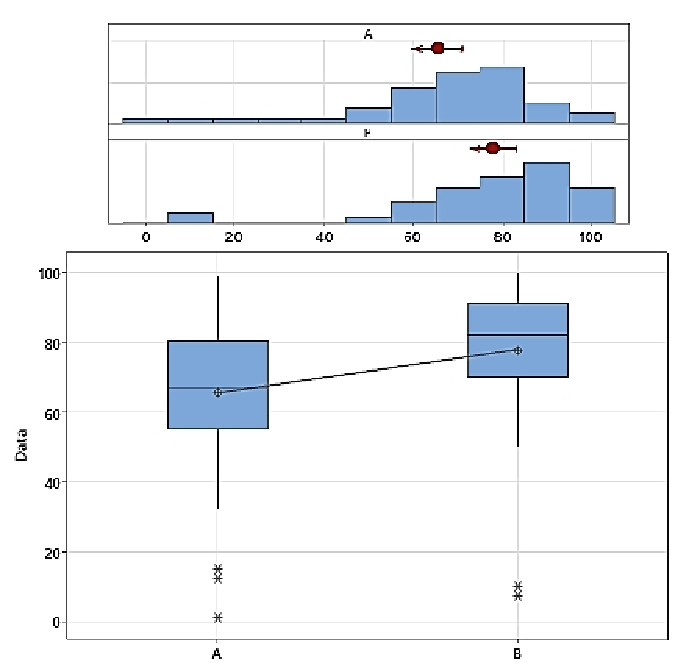
\includegraphics[width=0.72\linewidth]{fig11.pdf}
	\caption{Распределение итоговых оценок и ящичные диаграммы для групп A и B (тест на натуральные и целые числа, 0--100).}
	\label{fig11}
\end{figure}

\textbf{Улучшение внутри групп.}
Парные $t$-тесты показали высоко значимое улучшение в каждой группе и по обоим тестам ($p<0.001$): тест на мышление, группа~A $t(41)=9.92$ и группа~B $t(41)=9.97$ (оба $d_z\approx1.5$); тест на натуральные и целые числа, группа~A $t(41)=5.40$ ($d_z=0.83$) и группа~B $t(41)=6.02$ ($d_z=0.93$).

\textbf{Приросты оценок.}
Средние приросты в двух группах были почти одинаковыми (таблица~\ref{tab:descriptive}). Разность приростов ($B-A$) составила $-0.05$ балла по тесту на мышление (95\% ДИ $[-1.61,\,1.52]$; $t$ Уэлча $t(82.0)=-0.06$, $p=0.95$) и $0.52$ балла по тесту на натуральные и целые числа (95\% ДИ $[-8.29,\,9.34]$; $t(81.5)=0.12$, $p=0.91$). Тесты Манна--Уитни дали согласующиеся результаты ($p=0.97$ и $p=0.74$).

\textbf{ANCOVA (основной анализ).}
Итоговые оценки регрессировались на группу с предварительной оценкой в качестве ковариаты (таблица~\ref{tab:ancova}). Наклоны двух групп не различались (взаимодействие группа$\times$предварительная оценка $p=0.61$ для теста на мышление и $p=0.95$ для теста на натуральные и целые числа), так что предположение ANCOVA о параллельности наклонов выполняется. После корректировки различие между группами не было статистически значимым ни по одному из тестов, поэтому ни $H_{01}$, ни $H_{02}$ не отвергаются при $\alpha=0.05$.

\begin{table}[ht!]
	\centering
	\caption{ANCOVA итоговых оценок с предварительной оценкой в качестве ковариаты ($df=1,81$)}
	\label{tab:ancova}
	\footnotesize
	\setlength{\tabcolsep}{3pt}
	\renewcommand{\arraystretch}{1.25}
	\begin{tabular}{|p{3.3cm}|>{\centering\arraybackslash}p{2.3cm}|>{\centering\arraybackslash}p{3.0cm}|>{\centering\arraybackslash}p{1.1cm}|>{\centering\arraybackslash}p{1.1cm}|>{\centering\arraybackslash}p{1.9cm}|}
		\hline
		\textbf{Тест} & \textbf{Скоррект.\ средние (A, B)} & \textbf{Скоррект.\ $B-A$ [95\% ДИ]} & \textbf{$t(81)$} & \textbf{$p$} & \textbf{Частичный $\eta^2$} \\ \hline
		Мышление (0--12) & 8.25, 9.28 & 1.03 $[-0.21,\ 2.27]$ & 1.65 & 0.102 & 0.033 \\ \hline
		Натуральные и целые числа (0--100) & 68.48, 74.71 & 6.23 $[-1.42,\ 13.87]$ & 1.62 & 0.109 & 0.031 \\ \hline
	\end{tabular}
\end{table}

\textbf{Допущения.}
Тесты Шапиро--Уилка показали ненормальность итоговых оценок в обеих группах по обоим тестам ($p<0.01$), что отражает ограниченность шкал и эффекты потолка (5 учеников в группе~A и 9 в группе~B набрали максимум 12). Остатки ANCOVA были приблизительно нормальными для теста по шкале 0--100 ($p=0.14$), но не для дискретного 12-балльного теста ($p<0.001$); по этой причине ранговые проверки Манна--Уитни, приведённые выше, сообщаются наряду с параметрическими тестами, и они приводят к тем же выводам. По тесту на мышление корреляция между предварительными и итоговыми оценками была близка к нулю в обеих группах ($r=0.03$ и $r=-0.09$), поскольку предварительные оценки были низкими и сжатыми (средние 2.7--3.8 из 12), так что корректировка по ковариате там слабая.

\textbf{Чувствительность плана исследования.}
При $n=42$ в каждой группе и $\alpha=0.05$ в таблице~\ref{tab4} приведена наименьшая скорректированная разность, которую план мог обнаружить при заданной мощности (остаточные стандартные отклонения 2.78 и 17.05 балла).

\begin{table}[ht!]
	\centering
	\caption{Обнаруживаемая скорректированная разность $|\mu_B-\mu_A|$ в зависимости от мощности ($n=42$ в каждой группе, $\alpha=0.05$)}
	\label{tab4}
	\begin{tabular}{|c|c|c|}
		\hline
		\textbf{Мощность} & \textbf{Тест на мышление} & \textbf{Натуральные и целые числа} \\ \hline
		80\% & 1.72 & 10.55 \\
		90\% & 1.99 & 12.21 \\ \hline
	\end{tabular}
\end{table}

Наблюдаемые скорректированные разности (1.03 и 6.23 балла) меньше этих порогов, поэтому исследование не могло надёжно обнаружить эффекты такой величины, а доверительные интервалы в таблице~\ref{tab:ancova} не исключают умеренных преимуществ.

\textbf{Резюме и ограничения свидетельств.}
Если принимать результаты буквально, нескорректированное сравнение итоговых оценок по тесту на натуральные и целые числа говорит в пользу группы с головоломками ($p=0.0077$). Однако группа~B ещё до обучения опережала примерно на 12 баллов, и обе группы улучшили результат почти на одну и ту же величину (17.6 против\ 18.1 балла; 5.55 против\ 5.50 по тесту на мышление). После корректировки по предварительной оценке различие не является статистически значимым ни по одному из инструментов (скорректированное $+6.2$ балла, $p=0.109$; скорректированное $+1.0$ балл из 12, $p=0.102$). Точечные оценки говорят в пользу обучения на основе головоломок (скорректированное $d\approx0.37$ по обоим тестам), но совместимы с отсутствием эффекта. Значительное улучшение в обеих группах может отражать регулярное обучение, практику с тестом и созревание, которые в данном плане нельзя отделить от эффекта головоломок. Дополнительными ограничениями являются использование целых классов, одна школа, два раздела, три недели обучения и ненормальные ограниченные оценки. Поэтому результаты лучше рассматривать как предварительные и порождающие гипотезы; рекомендуется повторение исследования со случайным распределением и большей выборкой.
%%%%%%%%%%%%%%%NEW%%CHAPTER%%%%%%%%%%%%%%%%%%%%%%%
\chapter{Топологические индексы}~\label{sec5}
%-------------------------------------
Топологические индексы --- это числовые инварианты графа, получаемые из молекулярного графа химического соединения, предназначенные для количественной характеристики структурных особенностей и при этом
остающиеся неизменными при изоморфизме графов. В химической теории графов и хемоинформатике они лежат в основе исследований QSPR/QSAR~\cite{Todeschini2000}.
В этой главе изучаются индексы нерегулярности деревьев, связанных со словом Фибоначчи, и обсуждаются дистанционно-взвешенные и степенно-дистанционные дескрипторы.
%-------------------------------------
\section{Индексы нерегулярности деревьев и дерево факторов Фибоначчи}\label{sec5.1}

Все графы конечны и просты, $d_u$ --- степень вершины $u$, $m$ --- число рёбер. Мы используем индекс Альбертсона и индексы Загреба
\begin{equation}
	\operatorname{irr}(G)=\sum_{uv\in E}|d_u-d_v|,\qquad M_1(G)=\sum_{v}d_v^{2},\qquad M_2(G)=\sum_{uv\in E}d_ud_v ,
\end{equation}
и квадратичный вариант
\begin{equation}
	\operatorname{irr}_2(G)=\sum_{uv\in E}|d_u^{2}-d_v^{2}| .
\end{equation}

\begin{remark}
	В публикации~\cite{HamoudAbdullahCheb} индексы $\operatorname{FWI}$, $\operatorname{FWI}_t$ и $\operatorname{FWI}^*$ были введены для деревьев, вершины которых помечены словами Фибоначчи.
	Они зависят только от степеней дерева: $\operatorname{FWI}=\operatorname{FWI}_t=\operatorname{irr}$, а $\operatorname{FWI}^*$, определённый там через знаковые разности квадратов степеней вдоль ориентированных рёбер, совпадает с $\operatorname{irr}_2$ после взятия абсолютных значений.
	В данной диссертации мы используем только стандартные названия $\operatorname{irr}$ и $\operatorname{irr}_2$; слово Фибоначчи входит лишь через деревья из теоремы~\ref{thm:factortree}.
\end{remark}
%---------------------------------------------	
\subsection{Общие результаты}

\begin{proposition}~\label{pron1}
	Пусть $T$ --- дерево с максимальной степенью $\Delta$. Тогда $\operatorname{irr}_2(T)\ge\Delta(\Delta^2-1)$, причём равенство достигается тогда и только тогда, когда $T$ является путём или имеет ровно одну вершину степени больше $2$.
\end{proposition}

\begin{proof}
	Если $\Delta\le2$, то $T$ есть $K_2$ или путь $P_n$ ($n\ge3$), и $\operatorname{irr}_2(T)=0$ или $6=\Delta(\Delta^2-1)$. Пусть $\Delta\ge3$ и пусть $v$ имеет степень $\Delta$.
	Компоненты $B_1,\dots,B_\Delta$ графа $T-v$ присоединены к $v$ рёбрами $vx_i$; положим $E_i=E(B_i)\cup\{vx_i\}$, эти множества попарно не пересекаются.
	Каждая $B_i$ содержит висячую вершину $\ell_i$ дерева $T$, и вдоль пути $P_i$ от $v$ до $\ell_i$ неравенство треугольника даёт
	$\sum_{e\in P_i}|d_u^2-d_w^2|\ge\Delta^2-1$. Суммируя по $i$, получаем неравенство.
	Если некоторая $B_i$ содержит вершину $w$ степени $d_w\ge3$, возьмём $w$, ближайшую к $v$: путь $v\to w$ вносит вклад $\ge\Delta^2-d_w^2$, а два рёберно непересекающихся пути от $w$ до висячих вершин вносят $\ge d_w^2-1$ каждый,
	так что $E_i$ вносит $\ge\Delta^2+d_w^2-2>\Delta^2-1$, и неравенство строгое. В противном случае каждая вершина, отличная от $v$, имеет степень $\le2$, $T$ является пауком с центром $v$,
	каждая ножка имеет степени $\Delta,2,\dots,2,1$ (или $\Delta,1$), телескопические суммы являются равенствами и $\operatorname{irr}_2(T)=\Delta(\Delta^2-1)$.
\end{proof}

\begin{proposition}~\label{pron2}
	Для каждого дерева $T$ на $n\ge5$ вершинах, не являющегося путём, $\operatorname{irr}_2(P_n)<\operatorname{irr}_2(T)$.
\end{proposition}
\begin{proof}
	$\operatorname{irr}_2(P_n)=6$, тогда как дерево, не являющееся путём, имеет $\Delta\ge3$, так что $\operatorname{irr}_2(T)\ge24$ по предложению~\ref{pron1}.
\end{proof}

\Needspace{7\baselineskip}
\begin{proposition*}[Максимальность индекса звезды]
Для каждого дерева $T$ на $n\ge3$ вершинах, не изоморфного звезде $S_n$,
выполняется
\[
 \operatorname{irr}_2(T)<\operatorname{irr}_2(S_n)=n(n-1)(n-2).
\]
\end{proposition*}
\begin{proof}
Если $T$ не является звездой, его максимальная степень
$\Delta\le n-2$. Для любого ребра $uv$ степени его концов
лежат между $1$ и $\Delta$, поэтому
$|d_u^2-d_v^2|\le\Delta^2-1$.
Так как в дереве $n-1$ ребро, получаем
\[
 \operatorname{irr}_2(T)\le(n-1)(\Delta^2-1)
 \le(n-1)((n-2)^2-1)
 <(n-1)((n-1)^2-1).
\]
Последнее выражение равно индексу звезды.
Если для данного $n$ незвезды не существует, утверждение выполняется
в силу пустоты рассматриваемого класса.
\end{proof}

%----------------------------------------
\begin{lemma}~\label{lemn01}
	Пусть $G$ --- граф, а $\alpha,\beta$ --- несмежные вершины с $d_\alpha\ge d_\beta$. Пусть $r_\alpha$ ($r_\beta$) --- число соседей вершины $\alpha$ ($\beta$) со степенью больше $d_\alpha$ ($d_\beta$). Тогда
	\begin{equation}
		\operatorname{irr}_2(G+\alpha\beta)-\operatorname{irr}_2(G)=3d_\alpha(d_\alpha+1)+d_\beta(d_\beta-1)-2\bigl[(2d_\alpha+1)r_\alpha+(2d_\beta+1)r_\beta\bigr].
	\end{equation}
\end{lemma}
\begin{proof}
	Изменяются только новое ребро и рёбра при $\alpha$ и $\beta$. Новое ребро вносит $(d_\alpha+1)^2-(d_\beta+1)^2$. Для соседа $x$ вершины $\alpha$ слагаемое $|d_\alpha^2-d_x^2|$ становится $|(d_\alpha+1)^2-d_x^2|$:
	оно увеличивается на $2d_\alpha+1$, если $d_x\le d_\alpha$, и уменьшается на $2d_\alpha+1$, если $d_x>d_\alpha$; суммарно по $N(\alpha)$ это $(2d_\alpha+1)(d_\alpha-2r_\alpha)$. То же верно для $\beta$.
	Складывая: $(d_\alpha+1)^2-(d_\beta+1)^2+(2d_\alpha+1)(d_\alpha-2r_\alpha)+(2d_\beta+1)(d_\beta-2r_\beta)$, что упрощается до указанного выражения.
\end{proof}

\begin{example}[Звёзды]
	Для звезды $S_n$ ($n\ge2$): $\operatorname{irr}_2(S_n)=(n-1)((n-1)^2-1)=n(n-1)(n-2)$, $\operatorname{irr}(S_n)=(n-1)(n-2)$, следовательно, $\operatorname{irr}_2(S_n)-\operatorname{irr}(S_n)=(n-1)^2(n-2)\ge0$.
\end{example}
%----------------------------------------------	
\subsection{Деревья факторов штурмовых слов}

\begin{definition}
	Пусть $\mathbf u$ --- бесконечное слово и $n\ge2$. \emph{Дерево факторов} $T_n(\mathbf u)$ --- это корневое дерево, вершинами которого являются факторы слова $\mathbf u$ длины не более $n$
	(корнем служит пустое слово), где $w$ смежна с $wa$ ($a$ --- буква, $|wa|\le n$).
\end{definition}

Дерево зависит только от языка слова $\mathbf u$. Для штурмовых слов язык $\alpha$~зависит только от углового коэффициента; следовательно, можно взять $\mathbf u=\mathbf c_\alpha$, характеристическое слово.
Каждое характеристическое штурмово слово начинается с $x^dy$ для букв $x\ne y$ и некоторого $d\ge1$ (для слова Фибоначчи $\mathbf f$: $x=0$, $d=1$);
обмен двух букв не меняет дерево с точностью до изоморфизма.

\begin{theorem}\label{thm:factortree}
	Пусть $\mathbf c$ --- характеристическое штурмово слово, начинающееся с $x^dy$, $d\ge1$, и пусть $n\ge d+2$. Тогда
	\begin{equation}
		\begin{aligned}
 |V(T_n)|&=\frac{(n+1)(n+2)}2,\\
 \operatorname{irr}(T_n)&=4n-2d,\qquad
 \operatorname{irr}_2(T_n)=18n-10d-2.
\end{aligned}
	\end{equation}
	\begin{equation}
		M_1(T_n)=2n^2+8n-4,\qquad M_2(T_n)=2n^2+10n-11+d .
	\end{equation}
	В частности, для слова Фибоначчи ($d=1$): $\operatorname{irr}=4n-2$, $\operatorname{irr}_2=18n-12$, $M_2=2n^2+10n-10$.
\end{theorem}

\begin{proof}
	Мы используем два классических факта~\cite{Lothaire2002}: (F1) $\mathbf c$ имеет ровно $k+1$ факторов длины $k$, следовательно, ровно один правый специальный фактор $r_k$ (имеющий оба продолжения $r_kx$, $r_ky$) для каждого $k\ge0$, и $|V(T_n)|=\sum_{k=0}^n(k+1)$;
	(F2) $r_k$ есть обращение префикса длины $k$ слова $\mathbf c$: $r_k=\mathbf c[k-1]\cdots\mathbf c[0]$. В частности, $r_k=x^k$ при $k\le d$ и $r_{d+1}=y\,x^d$.
	
	\emph{Степени.} Корень имеет степень $2$. Вершина длины $k$, $1\le k\le n-1$, имеет степень $3$, если она есть $r_k$, и $2$ в противном случае; $n+1$ вершин длины $n$ являются висячими.
	
	\emph{Смежность специальных вершин.} $r_{k+1}=\mathbf c[k]\,r_k$, а дети $r_k$ суть $r_kx$, $r_ky$. Для $k\ge1$ имеем $r_{k+1}=r_ka$ для некоторой буквы $a$ тогда и только тогда, когда $\mathbf c[0..k]$ есть постоянное слово, т.е.\ тогда и только тогда, когда $k\le d-1$
	(тогда $r_{k+1}=r_kx$). Итак, $r_k$ и $r_{k+1}$ смежны в точности при $1\le k\le d-1$, и специальная вершина не имеет других специальных соседей.
	
	\emph{Веса рёбер} $|d_u-d_v|$ (далее все индексы таковы, что вершины существуют, что гарантируется условием $n\ge d+2$).
	(a) Ребро, входящее в $r_j$ ($1\le j\le n-1$): вес $1$, если его родитель есть корень ($j=1$) или неспециальная вершина ($j\ge d+1$), и $0$, если родитель есть $r_{j-1}$ ($2\le j\le d$). Всего $1+(n-1-d)=n-d$.
	(b) Два ребра, выходящие из $r_k$ при $1\le k\le n-2$: при $k\le d-1$ один ребёнок есть специальная $r_{k+1}$ (вес $0$), а другой неспециальный (вес $1$); при $d\le k\le n-2$ оба ребёнка неспециальные (вес $1$ каждое).
	Всего $(d-1)+2(n-1-d)$.
	(c) Два ребра из $r_{n-1}$ в висячие вершины: вес $2$ каждое, всего $4$.
	(d) Каждая из $p(n-1)-1=n-1$ неспециальных вершин длины $n-1$ имеет одного ребёнка-висячую вершину: вес $1$ каждое, всего $n-1$.
	Все остальные рёбра соединяют вершины степени $2$ и имеют вес $0$. Следовательно,
	\begin{equation}
		\operatorname{irr}(T_n)=(n-d)+(d-1)+2(n-1-d)+4+(n-1)=4n-2d .
	\end{equation}
	Для $\operatorname{irr}_2$ веса равны $|3^2-2^2|=5$, $|3^2-1|=8$, $|2^2-1|=3$; имеется $(n-d)+(d-1)+2(n-1-d)=3n-3-2d$ рёбер типа $(2,3)$, два типа $(3,1)$ и $n-1$ типа $(2,1)$:
	$\operatorname{irr}_2=5(3n-3-2d)+16+3(n-1)=18n-10d-2$.
	Последовательность степеней ($n(n-1)/2+1$ вершин степени $2$, $n-1$ степени $3$, $n+1$ висячих) даёт $M_1=2n^2+8n-4$, не зависящее от $d$.
	Для $M_2$ имеется $d-1$ рёбер типа $(3,3)$ (произведение $9$), $3n-3-2d$ типа $(2,3)$ (произведение $6$), $2$ типа $(3,1)$, $n-1$ типа $(2,1)$ и оставшиеся $\frac{n^2+3n}2-4n+3+d$ типа $(2,2)$ (произведение $4$);
	складывая, получаем $2n^2+10n-11+d$.
\end{proof}

\begin{table}[H]
	\centering
	\caption{Дерево $T_8$ для характеристических штурмовых слов с длиной первой серии $d$}
	\begin{tabular}{|c|c|c|c|c|c|}
		\hline
		$d$ & $|V|$ & $\operatorname{irr}$ & $\operatorname{irr}_2$ & $M_1$ & $M_2$ \\ \hline
		1 (Фибоначчи) & 45 & 30 & 132 & 188 & 198 \\ \hline
		2 & 45 & 28 & 122 & 188 & 199 \\ \hline
		3 & 45 & 26 & 112 & 188 & 200 \\ \hline
		4 & 45 & 24 & 102 & 188 & 201 \\ \hline
	\end{tabular}
\end{table}

\begin{remark}
	Индекс Альбертсона дерева факторов обнаруживает длину $d$ первой серии характеристического слова, т.е.\ первое неполное частное углового коэффициента ($d=a_1-1$ при $\alpha=[0;a_1,a_2,\dots]<\tfrac12$),
	тогда как $|V|$ и $M_1$ вообще не зависят от слова. Было бы интересно описать зависимость от последующих неполных частных для графов Рози штурмовых слов.
\end{remark}

%===========================
\subsection{Двумерная рекурсия и плотности её букв}\label{sec04}

\begin{definition}\label{newfibword}
	Пусть $a,b$ --- различные буквы. Определим $\mathscr T(0,v)=a$ при $v\ge1$, $\mathscr T(u,0)=b$ при $u\ge1$, и
	\begin{equation}
		\mathscr T(u,v)=\mathscr T(u-1,v)\,\mathscr T(u,v-1)\qquad(u,v\ge1).
	\end{equation}
	Например, $\mathscr T(1,1)=ab$, $\mathscr T(2,1)=abb$, $\mathscr T(1,2)=aab$, $\mathscr T(2,2)=aababb$.
\end{definition}

\begin{proposition}\label{newprove}
	При $u,v\ge1$: $|\mathscr T(u,v)|=\binom{u+v}{u}$, $\ |\mathscr T(u,v)|_a=\binom{u+v-1}{u}$, $\ |\mathscr T(u,v)|_b=\binom{u+v-1}{v}$.
	Следовательно, плотность $a$ в $\mathscr T(u,v)$ в точности равна $\dfrac{v}{u+v}$, а плотность $b$ равна $\dfrac{u}{u+v}$. Кроме того, $\dfrac1{2N}\log|\mathscr T(N,N)|\to\log2$.
\end{proposition}
\begin{proof}
	Каждая из трёх величин удовлетворяет рекуррентному соотношению Паскаля $x(u,v)=x(u-1,v)+x(u,v-1)$ при $u,v\ge1$ (пара $(0,0)$ никогда не используется), с граничными значениями
	$|{\cdot}|=1$, $|{\cdot}|_a=\binom{v-1}{0}=1,\ |{\cdot}|_b=0$ при $u=0$ и $|{\cdot}|=1$, $|{\cdot}|_a=0$, $|{\cdot}|_b=1$ при $v=0$, которые совпадают с граничными значениями указанных биномиальных коэффициентов.
	Плотность следует из $\binom{u+v-1}{u}=\frac{v}{u+v}\binom{u+v}{u}$. Наконец, $\binom{2N}{N}\sim4^N/\sqrt{\pi N}$ (Стирлинг).
\end{proof}
\begin{figure}[H]
	\centering
	\begin{tikzpicture}[scale=1.2, every node/.style={font=\small}]
		\draw[step=1.0,black,thin] (0,0) grid (5,5);
		\foreach \x in {0,...,4} {
			\node at (\x+0.5,-0.5) {$u=\x$};
		}
		\foreach \y in {0,...,4} {
			\node at (-0.5,\y+0.5) {$v=\y$};
		}
		\node at (0.5,0.5) {1};
		\foreach \i in {1,...,4} {
			\node at (\i+0.5,0.5) {1};
			\node at (0.5,\i+0.5) {1};
		}
		\node at (1.5,1.5) {2}; \node at (2.5,1.5) {3}; \node at (3.5,1.5) {4}; \node at (4.5,1.5) {5};
		\node at (1.5,2.5) {3}; \node at (2.5,2.5) {6}; \node at (3.5,2.5) {10}; \node at (4.5,2.5) {15};
		\node at (1.5,3.5) {4}; \node at (2.5,3.5) {10}; \node at (3.5,3.5) {20}; \node at (4.5,3.5) {35};
		\node at (1.5,4.5) {5}; \node at (2.5,4.5) {15}; \node at (3.5,4.5) {35}; \node at (4.5,4.5) {70};
		\foreach \i in {0,...,4} {
			\draw[red, thick] (\i,\i) rectangle ++(1,1);
		}
	\end{tikzpicture}
	\caption{Решётчатая сетка, иллюстрирующая длины $n(u,v)=\binom{u+v}{u}$ от $(0,0)$ до $(u,v)$. Диагональные клетки (выделенные красным) соответствуют центральным биномиальным коэффициентам.}
	\label{figlatticegrid}
\end{figure}
\begin{remark}
	Плотности точны и равны $\tfrac12$ на диагонали; они не включают золотое сечение. В частности, длины растут как $4^N$ вдоль диагонали, в отличие от слова Фибоначчи.
\end{remark}

%---------------------------------
\section{Индекс Альбертсона и локальная симметрия}

Индекс Альбертсона измеряет нерегулярность графа через разности степеней смежных вершин~\cite{Albertson1997}:
\begin{equation}
	A(G)=\operatorname{irr}(G)=\sum_{uv\in E}|d_G(u)-d_G(v)| .
\end{equation}
Он является чётным целым числом (так как $|x|\equiv x\pmod2$ и $\sum_{uv}(d_u+d_v)=\sum_v d_v^2\equiv2m$), и для \emph{связного} графа $A(G)=0$ тогда и только тогда, когда $G$ регулярен.

Для $P_4$ имеем $A(P_4)=1+0+1=2$.

Ребро $uv$ называется \emph{симметричным}, если $d_G(u)=d_G(v)$, и \emph{асимметричным} в противном случае; $A(G)$ есть сумма по асимметричным рёбрам.

\begin{proposition}
	Пусть $T$ --- дерево с $n\ge3$ вершинами и $\ell$ висячими вершинами. Тогда $A(T)\ge\ell$. Следовательно, $A(T)=2$ тогда и только тогда, когда $T$ есть путь $P_n$, и $A(T)\ge4$ для каждого другого дерева.
\end{proposition}
\begin{proof}
	При $n\ge3$ никакое ребро не соединяет две висячие вершины, и каждая висячая вершина смежна с вершиной степени $\ge2$, так что каждое из $\ell$ висячих рёбер имеет вес $\ge1$: $A(T)\ge\ell$. Теперь $\ell=2$ тогда и только тогда, когда $T=P_n$, и $A(P_n)=2$.
	Любое другое дерево имеет $\ell\ge3$, так что $A(T)\ge3$, следовательно, $A(T)\ge4$ по чётности.
\end{proof}
%---------------------------------
\section{Сигма-индекс и дистанционно-взвешенная нерегулярность}

Сигма-индекс~\cite{Gutman2018} определяется как
\begin{equation}
	\sigma(G)=\sum_{uv\in E}(d_G(u)-d_G(v))^2 ,
\end{equation}
и $\sigma(G)=0$ тогда и только тогда, когда связный граф $G$ регулярен. Для связного графа $G$ с расстояниями $d(u,v)$ и вещественного числа $\lambda$ мы предлагаем семейство
\begin{equation}
	A_\lambda(G)=\sum_{\{u,v\}\subseteq V}\frac{(d_G(u)-d_G(v))^2}{d(u,v)^{\lambda}} .
\end{equation}

\begin{proposition}
	(i) $A_0(G)=nM_1(G)-4m^2=n^2\operatorname{Var}(\text{degrees})$. (ii) $\lim_{\lambda\to\infty}A_\lambda(G)=\sigma(G)$. (iii) При $\lambda<0$ удалённые пары получают больший вес, чем близкие.
\end{proposition}
\begin{proof}
	(i) $\sum_{\{u,v\}}(d_u-d_v)^2=n\sum d_u^2-(\sum d_u)^2$. (ii) Слагаемые с $d(u,v)=1$ не зависят от $\lambda$ и в сумме дают $\sigma(G)$; каждое слагаемое с $d(u,v)\ge2$ не превосходит $\Delta^2/2^\lambda\to0$. (iii) Очевидно.
\end{proof}

\begin{example}
	Для $P_4$: $A_1(P_4)=1+\tfrac12+0+0+\tfrac12+1=3$.
\end{example}

\section{Индекс Гутмана}

Индекс Гутмана связного графа есть $\operatorname{Gut}(G)=\sum_{\{u,v\}}d_G(u)d_G(v)d(u,v)$ (\cite{Gutman1994}). Он отличается от степенно-дистанционного индекса (degree distance)
$\sum_{\{u,v\}}(d_u+d_v)d(u,v)$, в котором используется сумма степеней.

Для вещественного числа $\alpha$ положим $\operatorname{Gut}_\alpha(G)=\sum_{\{u,v\}}d_G(u)d_G(v)\,d(u,v)^\alpha$. Тогда $\operatorname{Gut}_1=\operatorname{Gut}$,
\begin{equation}
	\operatorname{Gut}_0(G)=\sum_{\{u,v\}}d_ud_v=\frac{4m^2-M_1(G)}2,\qquad
	\operatorname{Gut}_{-1}(G)=\sum_{\{u,v\}}\frac{d_ud_v}{d(u,v)} .
\end{equation}
\begin{example}
	$\operatorname{Gut}(P_4)=2+4+3+4+4+2=19$.
\end{example}
\noindent Семейства $A_\lambda$ и $\operatorname{Gut}_\alpha$ являются предлагаемыми обобщениями; их экстремальные свойства и связи с химическими данными остаются открытыми, и эти семейства предлагаются здесь для изучения.
%-----------------Finall chapter -------------
\chapter*{Заключение}
\addcontentsline{toc}{chapter}{Заключение}
%%%%%%%%%%%%%%%%%%%%%%%%%%%%%%%%%%%%%%%%%%%%%%
Данная диссертация выросла из одного вопроса: какова плотность нулей и единиц в подсловах слова Фибоначчи и в их палиндромах, и как эти плотности соотносятся? Этот вопрос, обманчиво простой по формулировке, раскрылся в ландшафт, значительно более богатый, чем ожидалось, и привёл от плотностей букв к палиндромным префиксам, избеганию повторений, инвариантам графов и метрической структуре на пространствах сдвигов. Мы подводим итог основным результатам в том порядке, в котором они возникали, и указываем направления, остающиеся открытыми.

Ответ на исходный вопрос дан в главе~3. Префикс длины $n$ слова Фибоначчи содержит ровно $\lfloor(n+1)/\varphi^{2}\rfloor$ единиц, и каждый фактор длины $m$ имеет плотности букв, отличающиеся от $1/\varphi^{2}$ и $1/\varphi$ не более чем на $1/m$, независимо от того, является ли он палиндромом (теорема~\ref{mainre}, предложение~\ref{prop:balance}). Близость плотностей подслов и их палиндромов, наблюдавшаяся в численных экспериментах, является, таким образом, следствием сбалансированности штурмовых слов, и никакого структурного различия между палиндромными и непалиндромными факторами не задействовано. Плотности, разумеется, не меняются при обращении.

Затем палиндромная структура изучалась на уровне префиксов. Показано, что асимптотическая плотность палиндромов слова Фибоначчи равна $1/\varphi$ (теорема~\ref{thm:palFib}), что является максимальным значением для непериодического слова, как установлено Фишлером; мы доказываем верхнюю оценку $\limsup n_{i+1}/n_i\le\varphi$ непосредственно из явного семейства палиндромных префиксов, тогда как нижняя оценка следует из оценки Фишлера.
Для слов, обрамлённых одной граничной буквой с каждой стороны, определена точная погрешность плотностей букв (теорема~\ref{thm1Asymptotic}): она односторонняя и имеет порядок $\varphi^{-m}$, тогда как необрамлённые слова сходятся со скоростью $\varphi^{-2m}$ с чередующимся знаком. Для тернарного фибоначчиподобного слова вычислены плотности букв и доказано, что его конечные слова богаты (теорема~\ref{thm:Yrich});
плотность палиндромных префиксов каждого характеристического штурмова слова выражена через цепную дробь углового коэффициента (теорема~\ref{thm:palSturm}).

Отступая от слова Фибоначчи к более широкому комбинаторному ландшафту, глава~2 анализирует бесконечное слово~$\mathfrak{F}_{b}$, определённое через конкатенацию представлений факториалов в системе счисления с основанием $b$. Установлены полная факторная сложность и полная арифметическая сложность, так что $\mathfrak{F}_{b}$ является дизъюнктивным: каждое конечное слово над алфавитом встречается как фактор. Это поучительно контрастирует со словом Фибоначчи, сложность которого минимальна среди апериодических слов.

Раздел~\ref{sec3.8} обращается к повторениям. Вводятся сильно $(k,\delta)$-свободные слова, и для обобщённых слов Туэ--Морса $W^{(b)}$ доказана полная классификация: сильные $(k,\sigma^j)$-повторы существуют тогда и только тогда, когда $k\le\kappa(N,b,j)$ (теорема~\ref{tw:main}); при $b=2$ слово является сильно $(3,\sigma^j)$-свободным тогда и только тогда, когда $j\not\equiv1\pmod N$ (теорема~\ref{avoidance}). Подсдвиг минимален, имеет нулевую энтропию и строго эргодичен (теорема~\ref{thm:dynWb}). Раздел~\ref{sec3.7} содержит символико-решёточную метрику $d_{SL}$, для которой подсдвиги компактны, а сдвиг является $2$-липшицевым. Глава~4 содержит решение задачи о минимальном разрезании полимино и экспериментальное исследование обучения на основе головоломок.

Глава~5 изучает индексы нерегулярности и индексы типа Загреба. Для деревьев факторов характеристических штурмовых слов, включая слово Фибоначчи, в замкнутой форме вычислены индекс Альбертсона, его квадратичный вариант и два индекса Загреба (теорема~\ref{thm:factortree}); индекс Альбертсона обнаруживает длину первой серии слова. Также приведены исправленная форма леммы о квадратичном индексе нерегулярности и характеризация случая равенства в нижней оценке для деревьев.

Наконец, раздел~\ref{sec4.3} сообщает о предварительном классном исследовании с сирийскими учениками шестого класса по обучению на основе головоломок. Нескорректированные итоговые оценки говорили в пользу группы с головоломками по одному инструменту, но эта группа также начинала с более высокого исходного уровня, а обе группы улучшили результат почти на одну и ту же величину; после учёта предварительных оценок оставшееся различие не было статистически значимым ни по одному инструменту. Поэтому исследование указывает на возможную пользу, с положительной, но статистически неубедительной оценкой, а не устанавливает её.

В совокупности эти результаты подтверждают, что исходный вопрос о плотностях, будучи разрешимым в собственных терминах, фактически был точкой входа в значительно более широкую теорию. Диссертация имеет один центральный объект --- семейство слов типа Штурма и Туэ--Морса, изучаемых через плотности, палиндромную структуру, повторения и инварианты графов.

Остаётся ряд естественных проблем. Факторная сложность $W_{A,\sigma,a_0}$ сопоставлена с известным результатом Тромпа--Шаллита~\cite{TrompShallit1995}; сильная $(k,\delta)$-свобода для перестановок $\delta$, не являющихся степенями $\sigma$, не рассматривается (раздел~\ref{sec3.8}). Максимальность $\operatorname{irr}_2(S_n)$ среди деревьев на $n$ вершинах доказана в главе~5. Зависимость более тонких графовых инвариантов от последующих неполных частных углового коэффициента остаётся предметом дальнейшего исследования.
Экстремальные свойства предлагаемых семейств $A_\lambda$ и $\operatorname{Gut}_\alpha$ ещё предстоит изучить. Эффект обучения на основе головоломок следует вновь исследовать в более крупном исследовании со случайным распределением и анализом с поправкой на исходный уровень.

Слово Фибоначчи начиналось в этой диссертации как объект изучения. Оно заканчивается как отправная точка.    

%###################################################
	\begin{thebibliography}{151}
		
		\bibitem{Abdullah}
		Abdullah D., Hamoud J. The density of zero and one in Fibonacci word for subwords and their palindromes. arXiv preprint arXiv:2507.19351. 2025.
		
		%\bibitem{AbdullahHamoud}
		%Abdullah D., Hamoud J. Density characterization with the upper bound of density of Fibonacci word. arXiv preprint arXiv:2509.00886. 2025.
		
		%\bibitem{Adamczewski}
		%Adamczewski B., Cassaigne J. On the transcendence of real numbers with a regular expansion // J. Number Theory. 2003. Vol. 103, No. 1. P. 27--37.
		
		\bibitem{AdamczewskiB2007}
		Adamczewski B., Bugeaud Y. On the complexity of algebraic numbers I: Expansions in integer bases // Annals of Mathematics. 2007. Vol. 165, No. 2. P. 547--565.
		
		\bibitem{Ahdhianto}
		Ahdhianto E., Marsigit, Haryanto, Nurfauzi Y. Improving fifth-grade students' mathematical problem-solving and critical thinking skills using problem-based learning // Universal J. Educ. Res. 2021. Vol. 8, No. 5. DOI: 10.13189/ujer.2020.080539.
		
		\bibitem{Albertson1997}
		Albertson M.O. The irregularity of a graph // Ars Combin. 1997. Vol. 46. P. 219--225.
		
		\bibitem{Allouche}
		Allouche J.P., Shallit J. Automatic Sequences: Theory, Applications, Generalizations. Cambridge University Press, 2003.
		
		\bibitem{AlloucheBaake}
		Allouche J.P., Baake M., Cassaigne J., Damanik D. Palindrome complexity // Theoret. Comput. Sci. 2003. Vol. 292, No. 1. P. 9--31. DOI: 10.1016/S0304-3975(01)00212-2.
		
		\bibitem{Almustafa}
		Almustafa A., Alashkar A. A prospectus for inclusion: Project study for a potential education solution for Syria's persons with disability (PwDs). OSF Preprints, 2020. DOI: 10.31235/osf.io/n394v.
		
		\bibitem{Alvarado}
		Alvarado R.C. What's so hard about the Monty Hall problem? arXiv preprint arXiv:2405.00884. 2024.
		
		\bibitem{Arnoux}
		Arnoux P., Rauzy G. Représentation géométrique de suites de complexité $2n+1$ // Bull. Soc. Math. France. 1991. Vol. 119, No. 2. P. 199--215.
		
		\bibitem{Avgustinovich}
		Avgustinovich S.V., Fon-Der-Flaass D.G., Frid A.E. Arithmetical complexity of infinite words // Words, Languages \& Combinatorics III. 2004. P. 51--62. DOI: 10.1142/9789812704979\_0004.
		
		\bibitem{Beatty1926}
		Beatty S. Problem 3173 // Amer. Math. Monthly. 1926. Vol. 33, No. 3. P. 159.
		
		\bibitem{Belov}
		Belov A.Y., Kondakov G.V., Mitrofanov I. Inverse problems of symbolic dynamics // Banach Center Publications. 2011. Vol. 94. P. 43--60.
		
		\bibitem{Berstel}
		Berstel J., Karhumäki J. Combinatorics on words: a tutorial // Bull. EATCS. 2003. Vol. 79. P. 9.
		
		\bibitem{Bevan}
		Bevan D. Threshold functions and the birthday paradox // The Mathematical Gazette, 2022. 106(566), 344–348. DOI: 10.1017/mag.2022.84.
		
		\bibitem{Boaler}
		Boaler J. Mathematical Mindsets: Unleashing Students' Potential through Creative Math, Inspiring Messages and Innovative Teaching // Jossey-Bass, 2016.
		
		\bibitem{Brinkhuis}
		Brinkhuis J. Nonrepetitive sequences on three symbols // Quart. J. Math. Oxford Ser. (2). 1983. Vol. 34, No. 2. P. 145--149. DOI: 10.1093/qmath/34.2.145.
		
		\bibitem{Cal}
		Mayor-Peña F., Barrera-Animas A.Y., Escobar-Castillejos D., Noguez J. Designing a gamified approach for digital design education aligned with Education 4.0 // Front. Educ. 2024. Vol. 9. DOI: 10.3389/feduc.2024.1439879.
		
		\bibitem{Danesi}
		Danesi M. An Anthropology of Puzzles: The Role of Puzzles in the Origins and Evolution of Mind and Culture. Routledge, 2020.
		
		\bibitem{Droubay}
		Droubay X., Justin J., Pirillo G. Episturmian words and some constructions of de Luca and {R}auzy // Theoret. Comput. Sci. 2001. Vol. 255, No. 1. P. 539--553. DOI: 10.1016/S0304-3975(99)00320-5.
		
		\bibitem{Droubay1995}
		Droubay X. Palindromes in the Fibonacci word // Inform. Process. Lett. 1995. Vol. 55, No. 4. P. 217--221.
		
		\bibitem{DroubayX}
		Droubay X., Pirillo G. Palindromes and Sturmian words // Theoret. Comput. Sci. 1999. Vol. 223, No. 1--2. P. 73--85. DOI: 10.1016/S0304-3975(97)00188-6.
		
		\bibitem{Duaa}
		Abdullah D., Hamoud J. The effect of using popular mathematical puzzles on the mathematical thinking of Syrian schoolchildren. arXiv preprint arXiv:2510.26263. 2025.
		
		\bibitem{Duaa23}
		Abdullah D., Meisami M. Factor and arithmetic complexity of concatenating the $n!$ // Chebyshevskii Sb. 2023. Vol. 24, No. 4. P. 341--344. DOI: 10.22405/2226-8383-2023-24-4-341-344.
		
		\bibitem{Falcon2007Plaza}
		Falcon S., Plaza A. On the Fibonacci $k$-numbers // Chaos Solitons Fractals. 2007. Vol. 32, No. 5. P. 1615--1624.
		
		\bibitem{Falcon2007PlazaSeco}
		Falcon S., Plaza A. $k$-Fibonacci sequences modulo $m$ // Chaos Solitons Fractals. 2009. Vol. 41, No. 1. P. 497--504. DOI: 10.1016/j.chaos.2008.02.014.
		
		\bibitem{Falcon2007PlazaThird}
		Falcon S., Plaza A. On $k$-Fibonacci sequences and polynomials and their derivatives // Chaos Solitons Fractals. 2007. Vol. 33, No. 3. P. 1005--1019.
		
		\bibitem{Feliciano}
		Feliciano-Semidei R., Wu K., Chaphalkar R.M. Introducing conditional probability using the Monty Hall problem // J. Univ. Teach. Learn. Pract. 2022. Vol. 19, No. 2. DOI: 10.53761/1.19.2.7.
		
		\bibitem{Fici2023}
		Fici G., Puzynina S. Abelian combinatorics on words: a survey // Comput. Sci. Rev. 2023. Vol. 47. Article 100532. DOI: 10.1016/j.cosrev.2022.100532.
		
		\bibitem{Fischler}
		Fischler S. Palindromic prefixes and episturmian words // J. Combin. Theory Ser. A. 2006. Vol. 113, No. 6. P. 1281--1304.
		
		\bibitem{Flores}
		Flores-Bascuñana M., Diago P.D., Villena-Taranilla R., Yáñez D.F. On augmented reality for the learning of 3D-geometric contents: A preliminary exploratory study with 6-grade primary students // Educ. Sci. 2020. Vol. 10, No. 1. DOI: 10.3390/educsci10010004.
		
		\bibitem{Fogg}
		Fogg N.P., Berthé V., Ferenczi S., Mauduit C., Siegel A. Substitutions in Dynamics, Arithmetics and Combinatorics. Vol. 1794. Springer, 2002.
		
		\bibitem{Glen2009}
		Glen A., Justin J., Widmer S., Zamboni L.Q. Palindromic richness // European J. Combin. 2009. Vol. 30, No. 2. P. 510--531.
		
		\bibitem{Grcar}
		Grcar J.F. Mathematics turned inside out: The intensive faculty versus the extensive faculty // High. Educ. 2011. Vol. 61. P. 693--720. DOI: 10.1007/s10734-010-9358-y.
		
		\bibitem{Grimm}
		Grimm U. Improved bounds on the number of ternary square-free words // J. Integer Seq. 2001. Vol. 4, No. 2. Article 01.2.7.
		
		\bibitem{Gutman1994}
		Gutman I. Selected properties of the Schultz molecular topological index // J. Chem. Inf. Comput. Sci. 1994. Vol. 34, No. 5. P. 1087--1089. DOI: 10.1021/ci00021a009.
		
		\bibitem{Gutman2018}
		Gutman I., Togan M., Yurttas A., Cevik A.S., Cangul I.N. Inverse problem for sigma index // MATCH Commun. Math. Comput. Chem. 2018. Vol. 79, No. 2. P. 491--508.
		
		\bibitem{HamoudAbdullah}
		Hamoud, J. and Abdullah, D., 2026. Analyze the Density of Words under Morphism $\{a, b\} $. arXiv preprint arXiv:2601.06150.
		
		\bibitem{HosseiniGutmanAhmadi}
		Hosseini S.A., Ahmadi M.B., Gutman I. Kragujevac trees with minimal atom-bond connectivity index // MATCH Commun. Math. Comput. Chem. 2014. Vol. 71. P. 5--20.
		
		\bibitem{Iortser}
		Iortser V., Abah J.A. Mathematical dimensions of Amenama Man Wankyo children play of the Tiv people // VillageMath Educ. Rev. 2022. Vol. 1. DOI: 10.2139/ssrn.4061834.
		
		\bibitem{Justin}
		Justin J., Pirillo G. Episturmian words and episturmian morphisms // Theoret. Comput. Sci. 2002. Vol. 276, No. 1--2. P. 281--313. DOI: 10.1016/S0304-3975(01)00207-9.
		
		\bibitem{knuth1997}
		Knuth D.E. The Art of Computer Programming: Fundamental Algorithms. Vol. 1. Addison-Wesley Professional, 1997.
		
		\bibitem{Kuipers}
		Kuipers L., Niederreiter H. Uniform Distribution of Sequences. John Wiley, 1974.
		
		\bibitem{Lothaire}
		Lothaire M. Combinatorics on Words. Cambridge University Press, 1997. DOI: 10.1017/CBO9780511566097.
		
		\bibitem{Lothaire1983}
		Lothaire M. Combinatorics on Words. Encyclopedia of Mathematics and its Applications, Vol. 17. Addison-Wesley, Reading, MA, 1983.
		
		\bibitem{Lothaire2002}
		Lothaire M. Algebraic Combinatorics on Words. Cambridge University Press, Vol. 90, 2002.
		
		\bibitem{Luo}
		Luo S., Wang D., Wang R. A study of gamified teaching activities for enhancing motivation in grade 6 primary school students // SHS Web Conf. 2023. Vol. 180. DOI: 10.1051/shsconf/202318004007.
		
		\bibitem{Mahalingam}
		Mahalingam K., Pandoh P. Counting scattered palindromes in a finite word. arXiv preprint arXiv:2108.02729. 2021.
		
		\bibitem{Marcus}
		Marcus B., Williams S. Symbolic dynamics // Scholarpedia. 2008. Vol. 3, No. 11. P. 2923.
		
		\bibitem{Maryana}
		Maryana M., Halim C., Rahmi H. The impact of gamification on student engagement and learning outcomes in mathematics education // Int. J. Bus. Law Educ. 2024. Vol. 5, No. 2. P. 1697--1708. DOI: 10.56442/ijble.v5i2.682.
		
		\bibitem{Maxfield}
		Maxfield E.J. A note on $n!$ // Math. Mag. 1970. Vol. 43. P. 64--67.
		
		\bibitem{Mehraban2006Gulliver}
		Mehraban E., Gulliver T.A., Hincal E. Blind signatures from the generalized $(t,k)$-Fibonacci $p$-sequences // J. Dyn. Games. 2026. Vol. 13. P. 193--203. DOI: 10.3934/jdg.2025022.
		
		\bibitem{Mendenhall}
		Mendenhall W., Beaver R.J., Beaver B.M. Introduction to Probability and Statistics. 13th ed. Cengage Learning, 2008.
		
		\bibitem{Mignosi}
		Mignosi F., Séébold P. Morphismes sturmiens et règles de Rauzy // J. Théor. Nombres Bordeaux. 1993. Vol. 5, No. 2. P. 221--233.
		
		\bibitem{Morse}
		Morse M., Hedlund G.A. Symbolic dynamics // Amer. J. Math. 1938. Vol. 60. P. 815--866.
		
		\bibitem{Morse1940}
		Morse M., Hedlund G.A. Symbolic dynamics II: Sturmian trajectories // Amer. J. Math. 1940. Vol. 62. P. 1--42.
		
		\bibitem{Niven}
		Niven I. The asymptotic density of sequences // Bull. Amer. Math. Soc. 1951. Vol. 57, No. 6. P. 420--434.
		
		\bibitem{Ochem}
		Ochem P., Reix T. Upper bound on the number of ternary square-free words // Proc. Workshop on Words and Automata (WOWA'06). 2006.
		
		\bibitem{Perrin}
		Berstel J., Perrin D. The origins of combinatorics on words // Eur. J. Comb. 2007. Vol. 28, No. 3. P. 996--1022. DOI: 10.1016/j.ejc.2005.07.019.
		
		\bibitem{Picciotto}
		Picciotto H., Pemantle R. There Is No One Way to Teach Math. Routledge, 2024. DOI: 10.4324/9781003473855.
		
		\bibitem{Pramestika}
		Pramestika N.P.D., Wulandari I.G.A.A., Sujana I.W. Enhancement of mathematics critical thinking skills through problem based learning assisted with concrete media // J. Educ. Technol. 2020. Vol. 4, No. 3. P. 254--263. DOI: 10.23887/jet.v4i3.25552.
		
		\bibitem{Puig}
		Puig A., Rodríguez I., Baldeón J., Múria S. Children building and having fun while they learn geometry // Comput. Appl. Eng. Educ. 2021. Vol. 30, No. 3. DOI: 10.1002/cae.22484.
		
		\bibitem{PulidoRamirez}
		Pulido J.F., Ramirez J.L., Vindas-Meléndez A.R. Generating trees and Fibonacci polyominoes. arXiv preprint arXiv:2411.17812. 2024.
		
		\bibitem{Rakshit}
		Rakshit U., Dwivedi N. What is the title of this paper? Solving logic puzzles using algorithms. arXiv preprint arXiv:2309.13044. 2023.
		
		\bibitem{Ramirez}
		Ramirez J.L., Rubiano G.N. On the $k$-Fibonacci words // Acta Univ. Sapientiae Inform. 2013. Vol. 5. P. 212--226. DOI: 10.2478/ausi-2014-0011.
		
		\bibitem{Rampersad2023Wiebe}
		Rampersad N., Wiebe M. Correlations of minimal forbidden factors of the Fibonacci word. arXiv preprint arXiv:2309.07070. 2023.
		
		\bibitem{Richard}
		Richard C., Grimm U. On the entropy and letter frequencies of ternary square-free words // Discrete Math. Theor. Comput. Sci. 2003. Vol. 6, No. 2. P. 313--324.
		
		\bibitem{Rigo}
		Rigo M. Formal Languages, Automata and Numeration Systems 1: Introduction to Combinatorics on Words. John Wiley \& Sons, 2014. DOI: 10.1002/9781119008200.
		
		\bibitem{Rigo2023}
		Rigo M., Stipulanti M., Whiteland M.A. Gapped binomial complexities in sequences // Proc. 2023 IEEE International Symposium on Information Theory (ISIT). 2023. P. 1294--1299. DOI: 10.1109/ISIT54713.2023.10206676.
		
		\bibitem{Shallit2022}
		Shallit J. The Logical Approach to Automatic Sequences: Exploring Combinatorics on Words with Walnut. London Mathematical Society Lecture Note Series, Vol. 482. Cambridge University Press, 2022.
		
		\bibitem{Shur}
		Shur A.M. Growth rates of complexity of power-free languages // Theoret. Comput. Sci. 2010. Vol. 411, No. 34--36. P. 3209--3223. DOI: 10.1016/j.tcs.2010.05.018.
		
		\bibitem{Thue}
		Thue A. Über unendliche Zeichenreihen // Norske Vid. Selsk. Skr. I. Mat. Nat. Kl. 1906. Vol. 7. P. 1--22.
		
		\bibitem{Thue1912}
		Thue A. Über die gegenseitige Lage gleicher Teile gewisser Zeichenreihen // Norske Vid. Selsk. Skr. Mat. Nat. Kl. 1912. Vol. 1. P. 1--67.
		
		\bibitem{Todeschini2000}
		Todeschini R., Consonni V. Handbook of Molecular Descriptors. Wiley-VCH, 2000. DOI: 10.1002/9783527613106.
		
		\bibitem{Trojovsky}
		Trojovsky P. On the natural density of sets related to generalized Fibonacci numbers of order $r$ // Axioms. 2021. Vol. 10, No. 3. Article 144. DOI: 10.3390/axioms10030144.
		
		\bibitem{Vuillon}
		Vuillon L. Balanced words // Bull. Belg. Math. Soc. Simon Stevin. 2003. Vol. 10, No. 5. P. 787--805. DOI: 10.36045/bbms/1074791332.
		
		\bibitem{Zolotov}
		Zolotov B. Another solution to the Thue problem of non-repeating words. arXiv preprint arXiv:1505.00019. 2015.
		
		\bibitem{Ferenczi}
		Ferenczi S., Mauduit C. Transcendence of numbers with a low complexity expansion // J. Number Theory. 67 (1997),  P.  146--161.
		
		\bibitem{DeLuca1997}
		de Luca A. Sturmian words: structure, combinatorics, and their arithmetics // Theoret. Comput. Sci. 1997. Vol. 183, No. 1. P. 45--82.
		
		\bibitem{Queffelec}
		Queff\'elec M. Substitution Dynamical Systems --- Spectral Analysis. Lecture Notes in Math., Vol. 1294. Springer, 1987 (2nd ed. 2010).
		
		\bibitem{Millin}
		Millin D. A. Problem H-237 // Fibonacci Quart. 1974, Vol. 12, P. 309.
		
		\bibitem{AbdullahHam}
		Abdullah D., Hamoud J. Generalized natural density DF($\mathfrak F_k$) of Fibonacci word // Vestnik KRAUNC. Fiz.-Mat. Nauki. 2025. Vol. 52, No. 3. P. 7--23. DOI: 10.26117/2079-6641-2025-52-3-7-23.
		
		\bibitem{HamoudAbdullahTver}
		Hamoud J., Abdullah D. On density and ergodic properties of the infinite Fibonacci word // Vestnik TvGU. Ser. Prikl. Mat. 2025. No. 4. P. 25--42. DOI: 10.26456/vtpmk742.
		
		\bibitem{KKT}
		Kohmoto M., Kadanoff L.P., Tang C. Localization problem in one dimension: mapping and escape // Phys. Rev. Lett. 1983. Vol. 50. P. 1870--1872.
		
		\bibitem{Ostlund}
		Ostlund S., Pandit R., Rand D., Schellnhuber H.J., Siggia E.D. One-dimensional Schr\"odinger equation with an almost periodic potential // Phys. Rev. Lett. 1983. Vol. 50. P. 1873--1876.
		
		\bibitem{ApostolicoFraenkel}
		Apostolico A., Fraenkel A.S. Robust transmission of unbounded strings using Fibonacci representations // IEEE Trans. Inform. Theory. 1987. Vol. 33, No. 2. P. 238--245.
		\bibitem{Crochemore}
		Crochemore M., Ilie L., Rytter W. Repetitions in strings: algorithms and combinatorics // Theoret. Comput. Sci. 2009. Vol. 410, No. 50. P. 5227--5235.
		
		\bibitem{HamoudAbdullahCheb}
		Hamoud J., Abdullah D. Irregularity and topological indices in Fibonacci word trees and modified Fibonacci word index // Chebyshevskii Sb. 2025. Vol. 26, No. 3. P. 257--273. DOI: 10.22405/2226-8383-2025-26-3-257-273.
		
	
\bibitem{Diaconis1977}
Diaconis P. The distribution of leading digits and uniform distribution mod~1 //
Ann. Probab. 1977. Vol.~5, No.~1. P.~72--81. DOI: 10.1214/aop/1176995891.
\bibitem{DamanikLenz2002}
Damanik D., Lenz D. The index of Sturmian sequences //
European J. Combin. 2002. Vol.~23. P.~23--29. DOI: 10.1006/eujc.2000.0496.
\bibitem{Peltomaki2015}
Peltomäki J. Characterization of repetitions in Sturmian words: A new proof //
Inform. Process. Lett. 2015. Vol.~115, No.~11. P.~886--891.
DOI: 10.1016/j.ipl.2015.05.011.
\bibitem{AdamczewskiAllouche2007}
Adamczewski B., Allouche J.-P. Reversals and palindromes in continued fractions //
Theoret. Comput. Sci. 2007. Vol.~380. P.~220--237.
DOI: 10.1016/j.tcs.2007.03.017.
\bibitem{TrompShallit1995}
Tromp J., Shallit J. Subword complexity of a generalized Thue--Morse word //
Inform. Process. Lett. 1995. Vol.~54, No.~6. P.~313--316.
DOI: 10.1016/0020-0190(95)00074-M.

\end{thebibliography}
	
\end{document}